 \documentclass[12pt]{book}
%https://www.overleaf.com/project/629e18789b6baeb860fd2545
\input{packages}
\input{packages-estudantes}

% define cores personalizadas para o texto de cada autor
\definechangesauthor[name={Jorge Henrique Cabral Fernandes}, color=orange]{jhcf} % git-user: jhcf
\definechangesauthor[name={Gabriel da Silva Corvino Nogueira}, color=orange]{nosgueira} % git-user: nosgueira
\definechangesauthor[name={Gabriel Ligoski}, color=blue]{gabrielligoski} % git-user: gabrielligoski
\definechangesauthor[name={Gustavo Rodrigues Gualberto}, color=green]{GustavoRGYGO} % git-user: GustavoRGYGO
\definechangesauthor[name={Edgar Sampaio de Barros}, color=green]{edgarsamp} % git-user: edgarsamp
\definechangesauthor[name={Erick Rodrigues Fraga}, color=green]{mutenesss} % git-user: mutenesss
\definechangesauthor[name={João Pedro de Sousa Soares Martins}, color=green]{jpssm} % git-user: jpssm
\definechangesauthor[name={Thiago Masera Tokarski}, color=green]{Toskosz} % git-user: Toskosz
\definechangesauthor[name={Marcelo Aiache Postiglione}, color=green]{marcelo3101} % git-user: marcelo3101
\definechangesauthor[name={Arthur Barreiros de Oliveira Mota}, color=purple]{BarreirosM} % git-user: BarreirosM
\definechangesauthor[name={Weliton César Pereira Barreto}, color=red]{welitonbarreto} % git-user: welitonbarreto
\definechangesauthor[name={Gabriel Pinheiro da Conceicao}, color=blue]{pinheirogh} % git-user: pinheirogh
\definechangesauthor[name={Breno Ribeiro Corrêa}, color=red]{brenoZ} % git-user: brenoZ
\definechangesauthor[name={João Victor de Souza Calassio}, color=blue]{jvcalassio} % git-user: jvcalassio
\definechangesauthor[name={Matheus Barbosa Santos}, color=cyan]{MatBSa} % git-user: MatBSa
\definechangesauthor[name={Plínio Candide Rios Mayer}, color=green]{PlinioMayer} % git-user: PlinioMayer
\definechangesauthor[name={Marco Antonio Nemetala Garcia}, color=green]{Hadeshade} % git-user: Hadeshade
\definechangesauthor[name={Regina Emy Da Nobrega Kamada}, color=orange]{bananaMoshpit} % git-user: bananaMoshpit
\definechangesauthor[name={Felipe Gomes Paradas}, color=purple]{fparadas} % git-user: fparadas
\definechangesauthor[name={Paulo Alvim Alvarenga}, color=yellow]{alvimpaulo} % git-user: alvimpaulo
\definechangesauthor[name={Marco Antônio Souza de Athayde}, color=pink]{masathayde} % git-user: masathayde
\definechangesauthor[name={João Antônio Desiderio de Moraes}, color=green]{joaoadm94} % git-user: joaoadm94
\definechangesauthor[name={Lucas de Oliveira Silva}, color=pink]{LuscasOSilva} % git-user: LuscasOSilva
\definechangesauthor[name={Isaque Augusto da Silva Santos}, color=pink]{seraphritt} % git-user: seraphritt
\definechangesauthor[name={Claudio Roberto Oliveira Peres de Barros}, color=pink]{ClaudioBarros} % git-user: ClaudioBarros
\definechangesauthor[name={André Cássio Barros de Souza}, color=pink]{andreloff} % git-user: andreloff
\definechangesauthor[name={Fernando Ferreira Cordeiro}, color=green]{FernandoCordeiro} % git-user: FernandoCordeiro
\definechangesauthor[name={Paulo Mauricio Costa Lopes}, color=orange]{RequiemDosVivos} % git-user: RequiemDosVivos
\definechangesauthor[name={Bruno Abreu Kamienski}, color=magenta]{brunosabreu} % git-user: brunosabreu
\definechangesauthor[name={André Fioravante Nicolodi Durante Júnior}, color=green]{AndreDuranteJr} % git-user: Andredurantejr

\definechangesauthor[name={Gabriel Teixeira Ribeiro}, color=blue]{moltentheory} % git-user: moltentheory

%MILLER, John H.; PAGE, Scott E. Complex Adaptive Systems: An introduction to computational models of social life. USA: Princeton University Press, 2007.


 

\makenoidxglossaries
\loadglsentries{1-Introducao/tarefas/T2-Glossario/estudantes/main}

\setcounter{tocdepth}{5}
\setcounter{secnumdepth}{5}
%\captionsetup[table]{name=Quadro}
\renewcommand{\lstlistingname}{Listagem de Código}

\newcommand{\dataset}{\textit{dataset}}
\newcommand{\query}{\textit{query}}
\newcommand{\githubusername}{\textless githubusername\textgreater}

\def\printpart{1} % Orientações Gerais, Introdução e Fundamentos de Pesquisa Bibliográfica

% Substitua o valor de printpart por 1, 2, 3, 4 ou 5, conforme a parte do documento que você quer gerar 
\def\printpart{1}

\setlength{\headheight}{73.04742pt}
\addtolength{\oddsidemargin}{-1.5cm}
\addtolength{\evensidemargin}{-1.5cm}
\addtolength{\textwidth}{3cm}
\addtolength{\topmargin}{-3cm}
\addtolength{\textheight}{2cm}

\addbibresource{RESIC.bib}
	
\begin{document}
\pagenumbering{gobble}% Remove page numbers (and reset to 1)
\clearpage
\thispagestyle{empty}

\begin{titlepage}
\begin{center}
 {\huge\bfseries \includegraphics[width=4cm]{unb-logo.jpg}\\
	CIC0203 - Computação Experimental - TA - 2022.2 - Notas e Registros
	\\Overleaf read only: \url{https://www.overleaf.com/read/rytgshjfsgpv}\\ 
	Github Repositório Origin (enviar tarefas aqui): \url{https://github.com/jhcf/Comput-Experim-20222}\\
	}

 % ----------------------------------------------------------------
 \vspace{1.5cm}
{\large	% author names and affiliations
	Jorge Henrique Cabral Fernandes (jhcf)\\
	Arthur Barreiros de Oliveira Mota (BarreirosM)\\
    Gabriel Pinheiro da Conceição (pinheirogh)\\
    Breno Ribeiro Corrêa (brenoZ)\\
    João Victor de Souza Calassio (jvcalassio)\\
    Matheus Barbosa Santos (MatBSa)\\
    Edgar Sampaio de Barros (edgarsamp) \\
    Felipe Gomes Paradas (fparadas) \\
    Marcelo Aiache Postiglione (marcelo3101) \\
    Paulo Alvim Alvarenga (alvimpaulo)\\
    Marco Antônio Souza de Athayde (masathayde)\\
    João Antonio Desidério de Moraes (joaoadm94)\\
    Gabriel da Silva Corvino Nogueira (nosgueira)\\
    Thiago Masera Tokarski (Toskosz)\\
    Erick Rodrigues Fraga (mutenesss)\\
    André Cássio Barros de Souza (andreloff)\\
    Lucas de Oliveira Silva (LuscasOSilva)\\
    João Pedro de Sousa Soares Martins (jpssm)\\
	Isaque Augusto da Silva Santos (seraphritt)\\
	Gustavo Rodrigues Gualberto (GustavoRGYGO)\\
    André Fioravante Nicolodi Durante Júnior (AndreDuranteJr)\\
	Cláudio Roberto Oliveira Peres de Barros (ClaudioBarros)\\ 
        Fernando Ferreira Cordeiro (FernandoCordeiro)\\
        Paulo Mauricio Costa Lopes (RequiemDosVivos)\\
	Bruno Abreu Kamienski (brunosabreu)\\
	Gabriel Teixeira Ribeiro\\
 }
	\vspace{1.5cm}
	{\large Brasília, \DTMnow}
\end{center}
\end{titlepage}
	%\date{10 de março de 2021}
	% make the title area
    %\maketitle
    \listoftodos
	\printnoidxglossary
	\tableofcontents
	\listoffigures
	\listoftables
	\clearpage
\pagenumbering{arabic}

\pagestyle{fancy}

	\chapter*{Resumo}

	Este documento contém notas de aula e registros em geral, produzidos de forma textual, pelo professor e turma da disciplina CIC0203 - Computação Experimental - TA - 2022.2.
	
	A disciplina adotará a abordagem de estudos estatísticos de simulações computacionais, como base para a construção de experimentos.

\part{Preparação\label{part:intro}}

    \chapter{Introdução à Simulação Multiagente em Python}

Conforme os argumentos no vídeo de \citet{crashcourse_controlled_2018}, filósofos e pensadores sobre tecnologia ponderam que no futuro o uso de simulações computacionais pode guiar muitas das experiências reais que vivenciaremos, e é possível que já estejamos vivendo essa experiencia sensorial, como se estivéssemos em uma ``Matrix''.

Este curso vai adotar essa hipótese como fundamento pedagógico, onde o estudante vai criar um laboratório de simulações para desenvolver e aprofundar sua compreensão do método experimental e de outras formas de investigação científica amparadas pelo computador.

Antes de entrarmos nos detalhes do método experimental, que vai ser apresentado em capítulo adiante, este texto vai lhe orientar sobre como criar simulações de sistemas multiagentes para exploração de fenômenos complexos, que serão posteriormente analisados de forma exploratória \citep{wickham_r_2016}, e depois de forma estatisticamente significativa \citep{goldstein_choosing_2015}.

Primeiro vamos falar sobre o que são simulações.
Depois sobre o que são simulações computacionais.
Depois sobre simulações multiagentes.
Por fim, vamos abordar como podem ser construídas simulações multiagentes com Python/MESA.
Ao final, você deverá ser capaz de fazer adaptações ao código de uma simulação multiagente em Python/MESA, para explorar um determinado fenômeno de seu interesse, com base em código já existente.

Nos capítulos seguintes, você aprenderá:
\begin{itemize}
    \item A projetar e codificar a manipulação de variáveis no seu modelo de simulação, que posteriormente serão consideradas variáveis independentes ou de controle de um experimento;
    \item A gerar massas de dados empíricos que podem ser analisadas por métodos e técnicas estatísticas.
\end{itemize}

Para concluir esta parte do curso sobre simulação, você deverá realizar uma tarefa em duas etapas, Tarefas 4.1 e 4.2, que vão evidenciar sua capacidade de fazer adaptações ao código de uma simulação multiagente em Python/MESA, para explorar de forma pré-experimental um determinado fenômeno de seu interesse, com base em código já existente.

\section{O que são simulações?}

Para uma ampla apresentação geral sobre simulação ver a Wikipedia em \url{https://en.wikipedia.org/wiki/Simulation}. Aqui apresentarei uma definição bem básica, suficiente para avançarmos:
Simulações são imitações da operação ou funcionamento de um sistema, fenômeno ou processo ao longo do tempo. 
As imitações são usualmente feitas com o uso de modelos, que podem ser mecânicos, computacionais etc. Um conjunto de pessoas também pode ser usado para realizar uma simulação, isso é, para imitar um sistema, como se um tipo de coreografia de dança. 
Para compreender a importância e o valor do desenvolvimento de modelos, ver \citet{epstein_why_2008}.

\section{O que são simulações computacionais?}

Simulações computacionais são aquelas produzidas com o uso de modelos computacionais, usualmente sistemas de software codificados para que o seu processamento de dados imite os passos de um sistema ou fenômeno qualquer, de natureza física, biológica, social, computacional etc, usando modelagem matemática. Esse programa de computador é chamado ``modelo de simulação computacional''
\citep{winsberg_computer_2019}. Cada execução do programa é chamado de ``uma simulação'' do sistema, ou do fenômeno ou do processo.

Para um vídeo bastante ilustrativo e curto (menos de 6 minutos) sobre a importância e oportunidade de realizar simulações computacionais, ver \citet{eaglin_introduction_2013}.

\section{O que são simulações baseadas em agentes?}

Existe dois tipos principais de simulações computacionais \citep{winsberg_computer_2019}:
\begin{description}
\item [Simulação Baseada em Equações] Esse tipo de simulação utiliza equações matemáticas (analíticas) que modelam fenômenos, usualmente fenômenos físicos, de modo que cada passo da simulação corresponde a avanços diferenciais na computação das imagens (outputs) da equação, em relação às variações nos domínios (inputs) da equação. \citet{winsberg_computer_2019} destaca que as equações podem se referir ao:
\begin{itemize}
    \item Comportamento de várias partículas individuais, ou;
    \item Comportamento de um fluido evoluindo ao longo do tempo.
\end{itemize}
Os engenheiros de áreas como Engenharia Civil e Mecânica, entre outros, usam muitas simulações desse tipo.

\item [Simulação Baseada em Agentes] Esse tipo de simulação é parecido com a simulação baseada em equações que determinam o comportamento de partículas individuais, só que na simulação baseada em agentes inexistem equações diferenciais globais que determinam o comportamento dos indivíduos \citep{winsberg_computer_2019}. Na simulação baseada em agentes, o comportamento dos agentes é determinado exclusivamente pelas regras locais que cada um segue (definidas por meio de algoritmos), as quais podem variar conforme o estado individual dos agentes. Esse tipo de simulação é ameno ao estudo de sistemas complexos adaptativos \citep{miller_complex_2007}, especialmente sistemas sociais, formados por seres humanos ou seres vivos, ou seja, partículas dotadas de agência ou inteligência.
\end{description}

Esse tipo de simulação é usado por cientistas sociais, e não tem tanta aplicação no campo das engenharias clássicas.

\section{Simulação Monte Carlo}

Nesta disciplina, trabalharemos primariamente com simulações baseadas em agentes, pela facilidade de adaptação dos programas desse tipo à proposta didática da disciplina, embora os princípios de experimentação também possam ser aplicáveis às simulações baseadas em equações.

Adicionalmente, um outro tipo de simulação computacional que não se enquadra na definição clássica de simulação (imitação de um fenômeno ou processo ao longo do tempo), mas que é fundamentada em princípios de estatística inferencial \textbf{que também utilizaremos para o teste de hipóteses sobre os dados dos experimentos a serem realizados} é a simulação do tipo Monte Carlo. 

Em simulações do tipo Monte Carlo não se está buscando imitar o processo ou comportamento de um fenômeno físico, químico ou social, mas sim calcular o valor de uma quantidade sobre o qual há uma grande incerteza envolvida, usando os conceitos de análise estatística de amostragens aleatórias de valores sobre uma população.

O trabalho que faremos na disciplina consistirá em usar os princípios da estatística inferencial usados na simulação Monte Carlo para  executar um conjunto de simulações multiagentes que vão guiar nossas experimentações para calcular as propriedades estatísticas do fenômeno simulado por simulação multiagentes.

\section{O que são simulações multiagentes?}

Simulações multiagentes são simulações baseadas em agentes, onde existem explicitamente regras de interações entre os agentes. Ou seja, onde os agentes se relacionam entre si, de modo que o comportamento de um é influenciado, em maior ou menor escala, pelo comportamento dos outros. 

Adicionalmente, as simulações (de sistemas) multiagentes são bastante adequadas para a modelagem de fenômenos sociais, especialmente sistemas sociais humanos, posto que esse tipo de modelo permite que cada agente siga suas regras individuais, o que se assemelha muito à forma como as pessoas se comportam em sociedade.

\section{Simulações multiagentes com Python/MESA}

MESA \citep{kazil_utilizing_2020} é um \textit{framework} de simulação multiagente escrito em Python, que tem bastante similaridade com outras linguagens, \textit{frameworks} e ferramentas como NetLogo \citep{wilensky_netlogo_1999},  

Para instalar mesa em uma versão específica, usando a versão 3.8 do Python, por exemplo, a versão com tag \verb|v0.9.0| use o comando abaixo.

\begin{verbatim}
    python3.8 -m pip install -e git+https://github.com/projectmesa/mesa@v0.9.0#egg=mesa
\end{verbatim}

\subsection{Exemplos de Simulações em Python/Mesa}

O framework Python/Mesa, ou simplesmente Mesa, possui um conjunto de simulações exemplo, que será usado para apoiar o desenvolvimento da experimentação computacional que você fará durante todo o restante da disciplina.

São os seguintes os exemplos de simulações construídas usando Mesa, disponíveis na distribuição padrão:
\begin{description}
\item [bank\_reserves] 

Descrição presente no código Python/Mesa: ``\textit{This model is a Mesa implementation of the Bank Reserves model from NetLogo. It is a highly abstracted, simplified model of an economy, with only one type of agent and a single bank representing all banks in an economy. People (represented by circles) move randomly within the grid. If two or more people are on the same grid location, there is a 50\% chance that they will trade with each other. If they trade, there is an equal chance of giving the other agent \$5 or \$2. A positive trade balance will be deposited in the bank as savings. If trading results in a negative balance, the agent will try to withdraw from its savings to cover the balance. If it does not have enough savings to cover the negative balance, it will take out a loan from the bank to cover the difference. The bank is required to keep a certain percentage of deposits as reserves and the bank's ability to loan at any given time is a function of the amount of deposits, its reserves, and its current total outstanding loan amount.}''. 

Para mais detalhes sobre esse modelo, ver a descrição do modelo no ambiente NetLogo, em 
\url{https://ccl.northwestern.edu/netlogo/models/BankReserves}.

\item [boltzmann\_wealth\_model] 

Descrição presente no código Python/Mesa: ``\textit{A simple model of an economy where agents exchange currency at random. All the agents begin with one unit of currency, and each time step can give a unit of currency to another agent. Note how, over time, this produces a highly skewed distribution of wealth.}''

Para uma explicação visual do conceito de Boltzmann aplicado à economia, ver \url{https://www.youtube.com/watch?v=BQrEEdy_uwM}.

\item [boltzmann\_wealth\_model\_network]

Descrição presente no código Python/Mesa: ``\textit{A simple model of an economy where agents exchange currency at random. All the agents begin with one unit of currency, and each time step can give a unit of currency to another agent. Note how, over time, this produces a highly skewed distribution of wealth. Network version}''

Para uma explicação visual do conceito de Boltzmann aplicado à economia, ver \url{https://www.youtube.com/watch?v=BQrEEdy_uwM}.
A diferença desse modelo em relação ao outro é o uso de uma rede de relacionamento entre os agentes. Para compreender a importância de um modelo baseado em redes, veja a introdução ao trabalho de \citet{pareschi_wealth_2014}.

\item [conways\_game\_of\_life] 

Descrição presente no código Python/Mesa: ``\textit{Represents the 2-dimensional array of cells in Conway's Game of Life.}''

Para uma apresentação detalhada do conceito dos jogos de Conway, veja \url{https://en.wikipedia.org/wiki/Conway's_Game_of_Life}.

\item [epstein\_civil\_violence] 

Descrição presente no código Python/Mesa: ``\textit{Model 1 from "Modeling civil violence: An agent-based computational approach," by Joshua Epstein. \url{http://www.pnas.org/content/99/suppl_3/7243.full} Attributes: height: grid height width: grid width citizen\_density: approximate \% of cells occupied by citizens. cop\_density: approximate \% of calles occupied by cops. citizen\_vision: number of cells in each direction (N, S, E and W) that citizen can inspect cop\_vision: number of cells in each direction (N, S, E and W) that cop can inspect legitimacy: (L) citizens' perception of regime legitimacy, equal across all citizens max\_jail\_term: (J\_max) active\_threshold: if (grievance - (risk\_aversion * arrest\_probability)) > threshold, citizen rebels arrest\_prob\_constant: set to ensure agents make plausible arrest probability estimates movement: binary, whether agents try to move at step end max\_iters: model may not have a natural stopping point, so we set a max.}''


\item [forest\_fire] 

Descrição presente no código Python/Mesa:``Simple Forest Fire model.''

Para explicação mais detalhada sobre os fundamentos do fenômeno e da simulação, ver \url{https://en.wikipedia.org/wiki/Forest-fire_model}.

\item [hex\_snowflake] 

Descrição presente no código Python/Mesa:``Represents the hex grid of cells. The grid is represented by a 2-dimensional array of cells with adjacency rules specific to hexagons.''

\item [pd\_grid] 

Descrição presente no código Python/Mesa:``Model class for iterated, spatial prisoner's dilemma model.''

Para uma introdução sobre o que é o dilema do prisioneiro, ver \url{https://www.youtube.com/watch?v=S52tJv7aMIE} e \url{https://webupon.com/blog/iterated-prisoners-dilemma-game/}.

\item [schelling] 

Descrição presente no código Python/Mesa:``Model class for the Schelling segregation model.''

Para uma discussão mais aprofundada sobre o trabalho de Schelling e seus modelos de segregação em \url{https://en.wikipedia.org/wiki/Thomas_Schelling#Models_of_segregation}.

\item [sugarscape\_cg] 

Descrição presente no código Python/Mesa: ``\textit{Sugarscape 2 Constant Growback}''.

Para uma apresentação detalhada do modelo Sugarscape ver \url{https://en.wikipedia.org/wiki/Sugarscape}.


\item [virus\_on\_network] 

Descrição presente no código Python/Mesa:``\textit{A virus model with some number of agents entering in contact through a network of relations}''

Para uma introdução mais aprofundada ver: \url{https://www.ncbi.nlm.nih.gov/pmc/articles/PMC7770744/pdf/41109_2020_Article_344.pdf}.

\item [wolf\_sheep] 

Descrição presente no código Python/Mesa:``\textit{A model for simulating wolf and sheep (predator-prey) ecosystem modelling.}''

Para mais detalhes, ver a apresentação em \url{https://sites.google.com/site/biologydarkow/ecology/predator-prey-simulation-of-the-lotka-volterra-model}.

\end{description}


    \chapter{Tarefa 8 - Teste Estatístico de Hipóteses - Parte 1. 15 pontos\label{tarefa:teste:hipotese:R}}

Antes de realizar essa tarefa, veja atentamente as instruções do capítulo anterior: "Conceitos Centrais em Estatística Inferencial".

Nessa tarefa você vai criar um novo capítulo, a partir do desenvolvido na tarefa anterior, com um conjunto de mais seis seções, após a atual seção "Conclusão" do capítulo do seu laboratório, conforme as seguintes orientações:
%como no modelo da seção \ref{tarefa:teste:hipotese:R:jhcf}, contendo um %texto com as seguintes características:
\begin{enumerate}
    \item Renomeie a atual seção "Conclusões" do seu capítulo, para "Conclusões Preliminares"; 
    \item Acrescente as seguintes seções ao seu capítulo:
    \begin{description}
        \item [Apresentação das Amostras] Nessa seção, refine o que antes era apenas a apresentação das "Variáveis Dependentes e Independentes", e realize a apresentação das amostras. 
        Descreva cuidadosamente as amostras coletadas, apresentando cada uma das colunas da planilha de amostras de experimentos por você coletadas, e faça uma descrição detalhada de cada coluna, que contenha:
        \begin{itemize}
            \item O nome da variável;
            \item O que significa a variável;
            \item Se a variável é para uso interno do simulador, variável de controle no experimento, variável independente ou variável dependente;
            \item As faixas de valores ou categorias dos registros obtidos, para fins de interpretação dos números (ex: Se umidade = 0, o que isso significa? Se umidade = 1, o que significa?;
        \end{itemize}
        
        Além disso, apresente os gráficos de distribuição de frequências para pelo menos quatro conjuntos de registros que contenham os mesmos valores para as variáveis independentes. Cada um desses conjuntos de registros será doravante chamados de Amostra.
        
        \item [Primeira Declaração Formal de Hipóteses] Supondo que foi feita a escolha inicial do teste t de Student, para comparar médias entre duas amostras (conjunto de registros) de variável dependente, que foram obtidas a partir de estímulos com diferentes valores para pelo menos uma variável independente, faça uma declaração de hipóteses nula e alternativa para o seu teste. Aplique corretamente os conceitos de hipóteses nula e alternativa, conforme o vídeo sobre Inferência Estatística.
        \item [Aplicação do Teste t] Use as instruções em \url{https://stat.ethz.ch/R-manual/R-devel/library/stats/html/t.test.html}, e com base no vídeo sobre teste t (\url{https://www.youtube.com/watch?v=AgDC9yoopUA}), apresente duas diferentes execuções do teste, comparando diferentes amostras. Apresente, usando lstlistings, todo o código R usado, os resultados apresentados no Console do R, e sua interpretação dos resultados. Informe sobre a comprovação ou rejeição da hipótese nula;
        \item [Segunda Declaração Formal de Hipóteses] Supondo que agora vais fazer uma análise de regressão linear, com as mesmas amostras, veja o vídeo e o texto sobre regressão linear em R:
        \begin{itemize}
            \item \url{https://www.youtube.com/watch?v=u1cc1r_Y7M0}; e
            \item \url{https://www.r-tutor.com/elementary-statistics/simple-linear-regression/significance-test-linear-regression}.
        \end{itemize}
        Com base nos vídeos, faça uma declaração de hipóteses nula e alternativa para o seu teste, que estabeleça possível relação linear entre uma variável independente e uma dependente. Aplique corretamente os conceitos de hipóteses nula e alternativa.
        \item [Aplicação do teste de regressão linear] Apresente duas diferentes execuções do teste, comparando diferentes amostras por meio de regressão linear. Apresente todo o código R dos comandos e dos resultados apresentados no Console do R, e sua interpretação dos resultados, sobre a comprovação ou não da hipótese nula;
        \item [Conclusões] Apresente suas conclusões sobre os testes realizados.
    \end{description}
 \end{enumerate}
    


    \chapter{O que é a Ciência?\label{ciência:o:que:eh}}

Existem várias definições sobre o que é a ciência. Algumas questões sobre essa definição são apresentadas por \citep{fernandes_consideracoes_2021}, cujo texto está reproduzido a seguir. 

A figura \ref{fig:ciencia-filosofia}~ apresenta um mapa conceitual que trata da fundamentação do conceito de ciência e sua relação com a filosofia.
Veja o vídeo da aula de 20 de janeiro de 2022, para mais detalhes.

\begin{figure}[ht]
    \centering
    \caption{Conceitos fundamentais de ciência, e sua relação com a filosofia}
    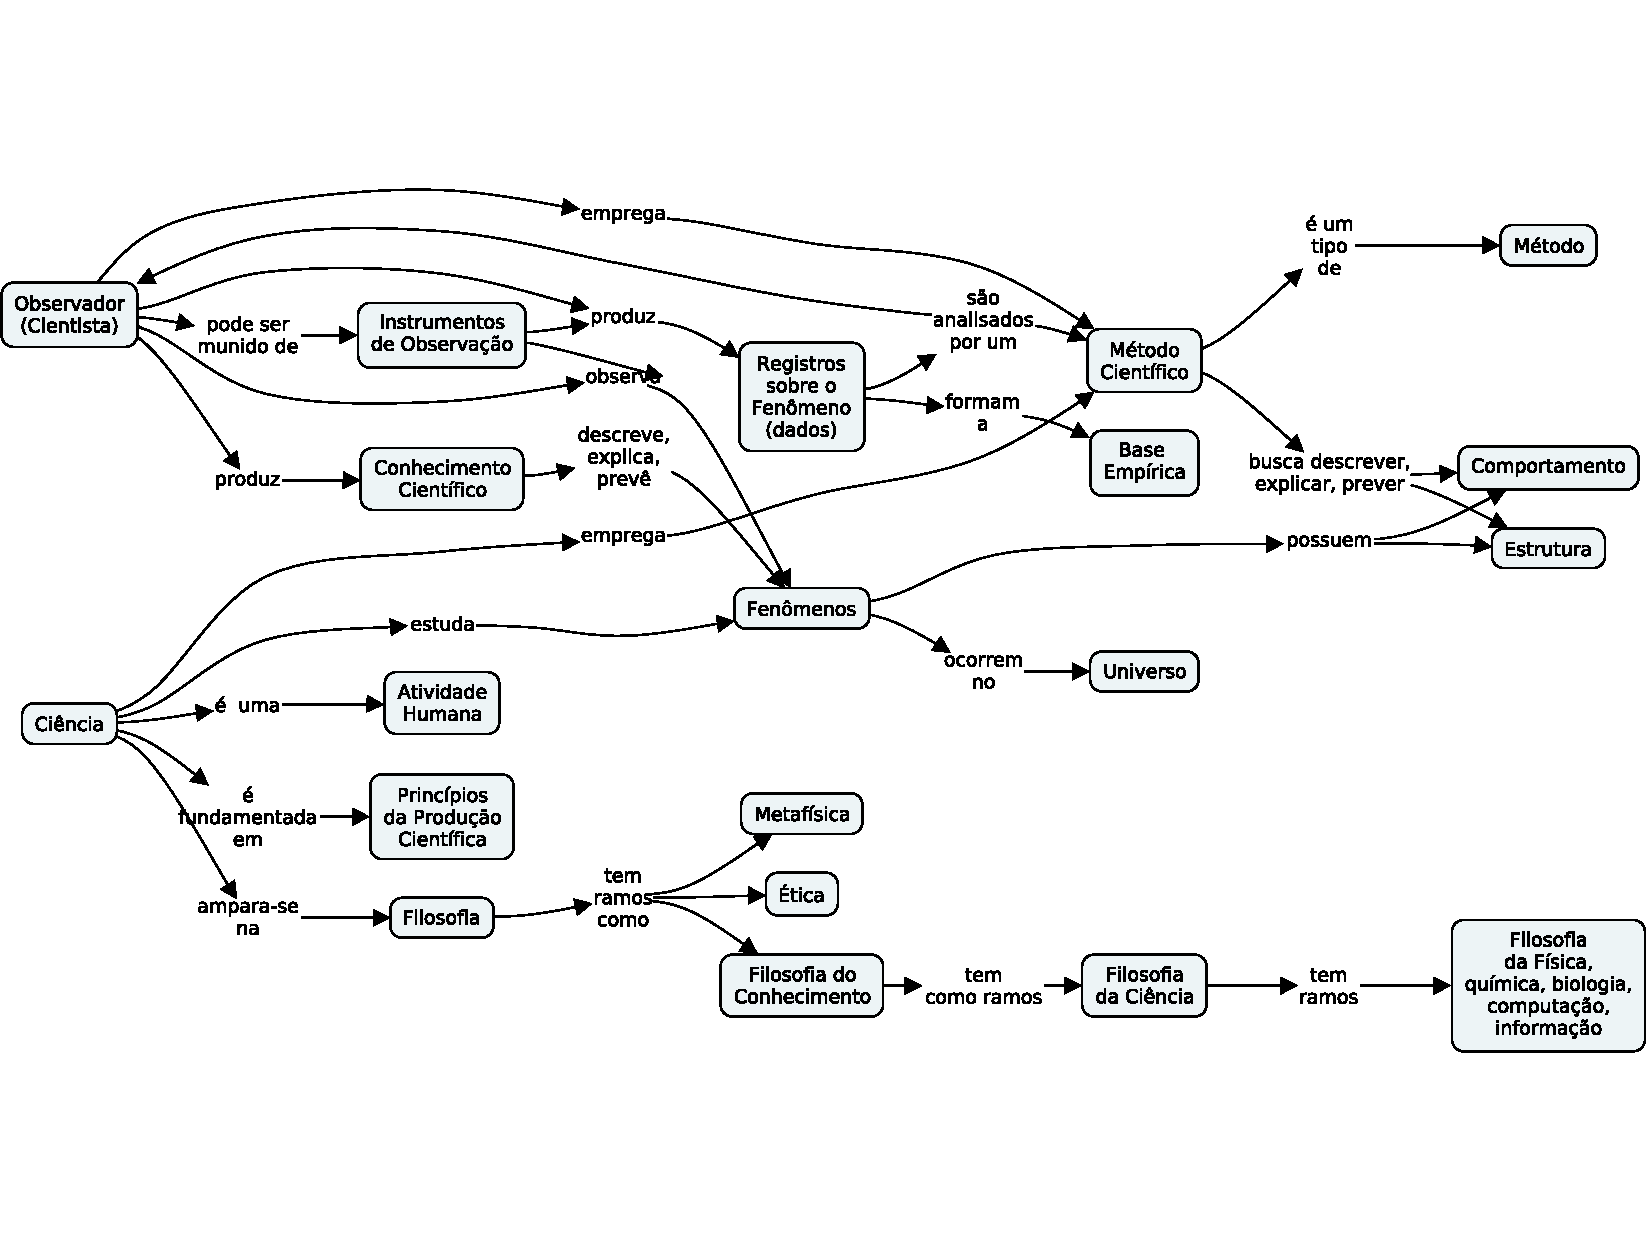
\includegraphics[page=1,angle=90,width=0.9\textwidth,height=0.9\textheight]{1-Introducao/aulas/Ciencia-e-Filosofia.pdf}
    \label{fig:ciencia-filosofia}
\end{figure}

A figura \ref{fig:desenv-sw-ciencia-filosofia} acrescenta à figura  \ref{fig:ciencia-filosofia}~ os conceitos que relacionam a natureza do desenvolvimento de software à  fundamentação do conceito de ciência e sua relação com a filosofia.
Veja o vídeo  da aula de 20 de janeiro de 2022, para mais detalhes.

\begin{figure}[ht]
    \centering
    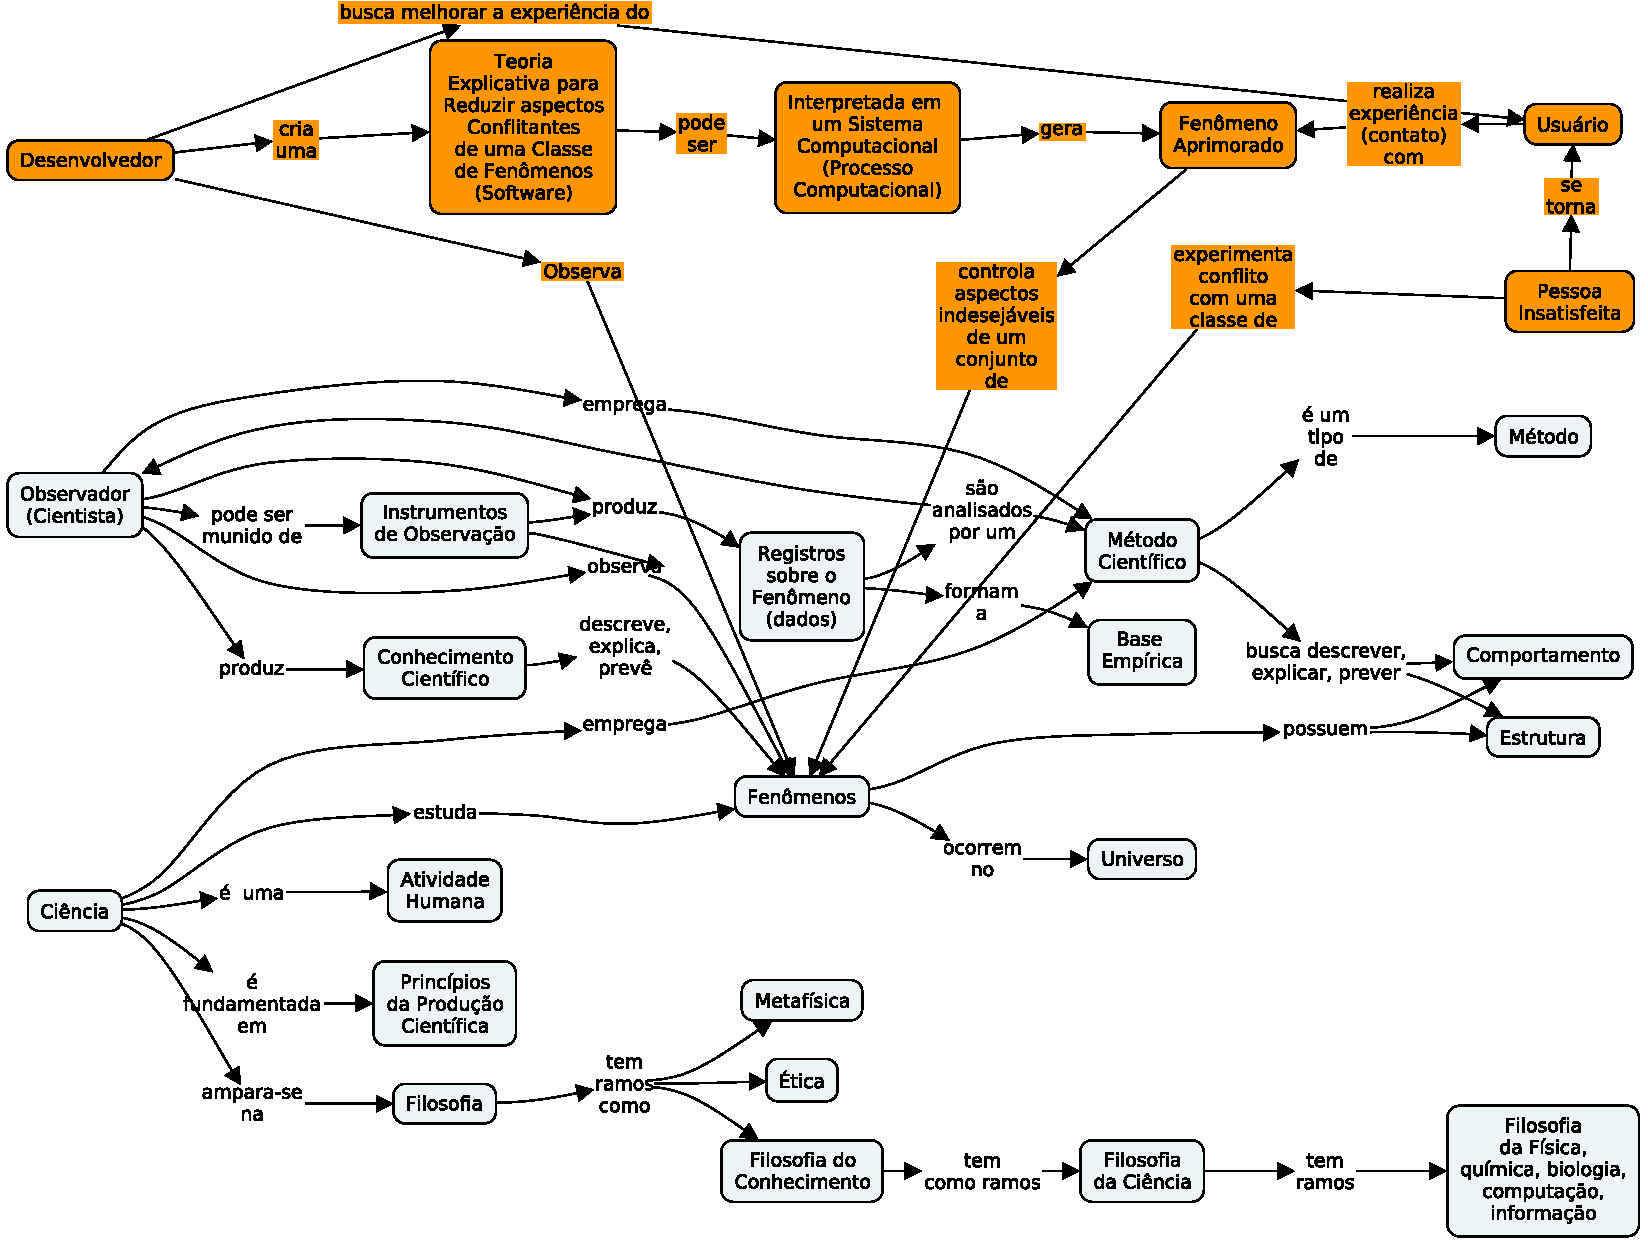
\includegraphics[page=1,angle=90,width=0.8\textwidth,height=0.9\textheight]{1-Introducao/aulas/Desenvolvimento-de-Software-Ciencia-e-Filosofia.pdf}
    \caption{Como a atividade do desenvolvimento de software se compara à atividade cientifica? Fonte: jhcf}
    \label{fig:desenv-sw-ciencia-filosofia}
\end{figure}

A figura \ref{fig:principios:ativ:cientifica}~ sumariza, em um mapa conceitual, os princípios da atividade científica e os relaciona com os princípios do desenvolvimento de software.
Veja o vídeo da aula de 20 de janeiro de 2022, para mais detalhes.

\begin{figure}[ht]
    \centering
    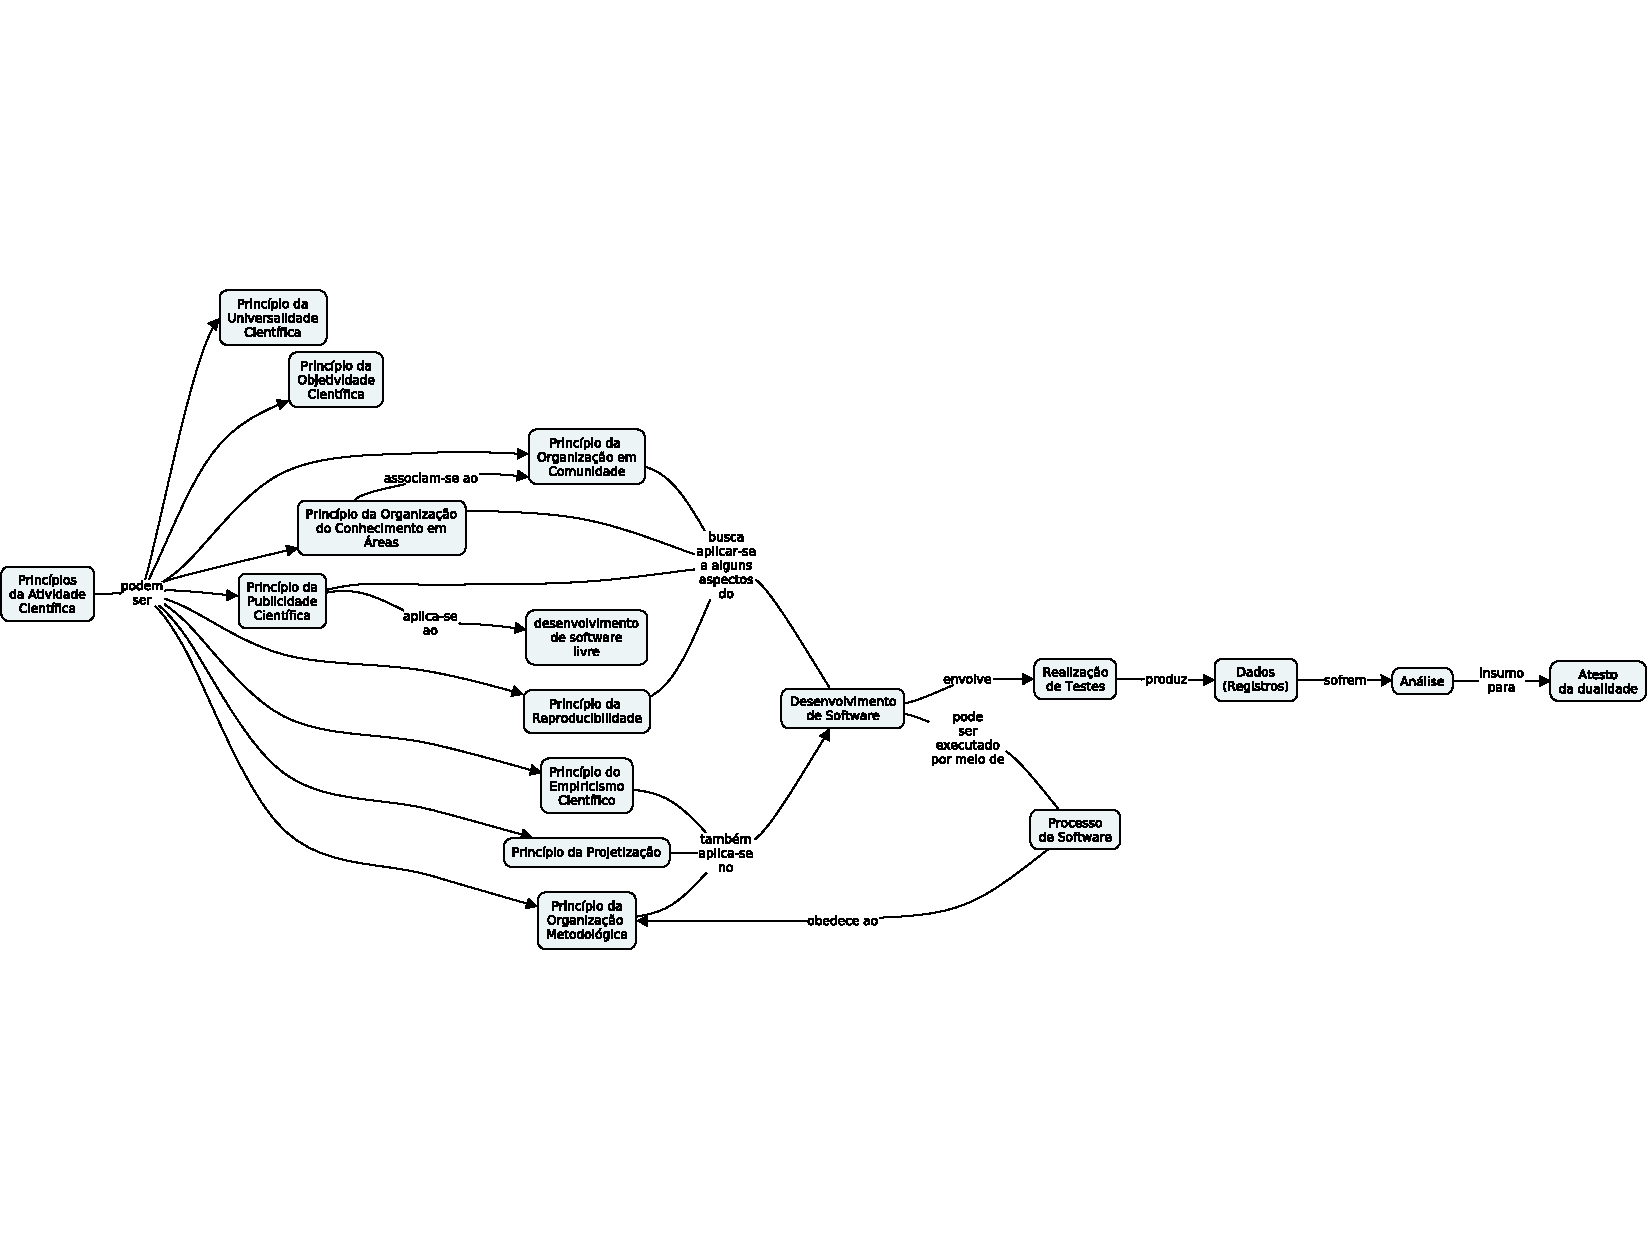
\includegraphics[page=1,angle=90,width=0.9\textwidth,height=0.9\textheight]{1-Introducao/aulas/Principios-da-atividade-cientifica.pdf}
    \caption{Quais os princípios da  atividade cientifica? como se relacionam com a atividade de desenvolvimento de software. Fonte: jhcf}
    \label{fig:principios:ativ:cientifica}
\end{figure}


	\includepdf[pages=-]{1-Introducao/aulas/Ciencia-e-sua-Avaliacao} 
    \chapter{Tarefa 8 - Teste Estatístico de Hipóteses - Parte 1. 15 pontos\label{tarefa:teste:hipotese:R}}

Antes de realizar essa tarefa, veja atentamente as instruções do capítulo anterior: "Conceitos Centrais em Estatística Inferencial".

Nessa tarefa você vai criar um novo capítulo, a partir do desenvolvido na tarefa anterior, com um conjunto de mais seis seções, após a atual seção "Conclusão" do capítulo do seu laboratório, conforme as seguintes orientações:
%como no modelo da seção \ref{tarefa:teste:hipotese:R:jhcf}, contendo um %texto com as seguintes características:
\begin{enumerate}
    \item Renomeie a atual seção "Conclusões" do seu capítulo, para "Conclusões Preliminares"; 
    \item Acrescente as seguintes seções ao seu capítulo:
    \begin{description}
        \item [Apresentação das Amostras] Nessa seção, refine o que antes era apenas a apresentação das "Variáveis Dependentes e Independentes", e realize a apresentação das amostras. 
        Descreva cuidadosamente as amostras coletadas, apresentando cada uma das colunas da planilha de amostras de experimentos por você coletadas, e faça uma descrição detalhada de cada coluna, que contenha:
        \begin{itemize}
            \item O nome da variável;
            \item O que significa a variável;
            \item Se a variável é para uso interno do simulador, variável de controle no experimento, variável independente ou variável dependente;
            \item As faixas de valores ou categorias dos registros obtidos, para fins de interpretação dos números (ex: Se umidade = 0, o que isso significa? Se umidade = 1, o que significa?;
        \end{itemize}
        
        Além disso, apresente os gráficos de distribuição de frequências para pelo menos quatro conjuntos de registros que contenham os mesmos valores para as variáveis independentes. Cada um desses conjuntos de registros será doravante chamados de Amostra.
        
        \item [Primeira Declaração Formal de Hipóteses] Supondo que foi feita a escolha inicial do teste t de Student, para comparar médias entre duas amostras (conjunto de registros) de variável dependente, que foram obtidas a partir de estímulos com diferentes valores para pelo menos uma variável independente, faça uma declaração de hipóteses nula e alternativa para o seu teste. Aplique corretamente os conceitos de hipóteses nula e alternativa, conforme o vídeo sobre Inferência Estatística.
        \item [Aplicação do Teste t] Use as instruções em \url{https://stat.ethz.ch/R-manual/R-devel/library/stats/html/t.test.html}, e com base no vídeo sobre teste t (\url{https://www.youtube.com/watch?v=AgDC9yoopUA}), apresente duas diferentes execuções do teste, comparando diferentes amostras. Apresente, usando lstlistings, todo o código R usado, os resultados apresentados no Console do R, e sua interpretação dos resultados. Informe sobre a comprovação ou rejeição da hipótese nula;
        \item [Segunda Declaração Formal de Hipóteses] Supondo que agora vais fazer uma análise de regressão linear, com as mesmas amostras, veja o vídeo e o texto sobre regressão linear em R:
        \begin{itemize}
            \item \url{https://www.youtube.com/watch?v=u1cc1r_Y7M0}; e
            \item \url{https://www.r-tutor.com/elementary-statistics/simple-linear-regression/significance-test-linear-regression}.
        \end{itemize}
        Com base nos vídeos, faça uma declaração de hipóteses nula e alternativa para o seu teste, que estabeleça possível relação linear entre uma variável independente e uma dependente. Aplique corretamente os conceitos de hipóteses nula e alternativa.
        \item [Aplicação do teste de regressão linear] Apresente duas diferentes execuções do teste, comparando diferentes amostras por meio de regressão linear. Apresente todo o código R dos comandos e dos resultados apresentados no Console do R, e sua interpretação dos resultados, sobre a comprovação ou não da hipótese nula;
        \item [Conclusões] Apresente suas conclusões sobre os testes realizados.
    \end{description}
 \end{enumerate}
    

    
    \chapter{Tarefa 8 - Teste Estatístico de Hipóteses - Parte 1. 15 pontos\label{tarefa:teste:hipotese:R}}

Antes de realizar essa tarefa, veja atentamente as instruções do capítulo anterior: "Conceitos Centrais em Estatística Inferencial".

Nessa tarefa você vai criar um novo capítulo, a partir do desenvolvido na tarefa anterior, com um conjunto de mais seis seções, após a atual seção "Conclusão" do capítulo do seu laboratório, conforme as seguintes orientações:
%como no modelo da seção \ref{tarefa:teste:hipotese:R:jhcf}, contendo um %texto com as seguintes características:
\begin{enumerate}
    \item Renomeie a atual seção "Conclusões" do seu capítulo, para "Conclusões Preliminares"; 
    \item Acrescente as seguintes seções ao seu capítulo:
    \begin{description}
        \item [Apresentação das Amostras] Nessa seção, refine o que antes era apenas a apresentação das "Variáveis Dependentes e Independentes", e realize a apresentação das amostras. 
        Descreva cuidadosamente as amostras coletadas, apresentando cada uma das colunas da planilha de amostras de experimentos por você coletadas, e faça uma descrição detalhada de cada coluna, que contenha:
        \begin{itemize}
            \item O nome da variável;
            \item O que significa a variável;
            \item Se a variável é para uso interno do simulador, variável de controle no experimento, variável independente ou variável dependente;
            \item As faixas de valores ou categorias dos registros obtidos, para fins de interpretação dos números (ex: Se umidade = 0, o que isso significa? Se umidade = 1, o que significa?;
        \end{itemize}
        
        Além disso, apresente os gráficos de distribuição de frequências para pelo menos quatro conjuntos de registros que contenham os mesmos valores para as variáveis independentes. Cada um desses conjuntos de registros será doravante chamados de Amostra.
        
        \item [Primeira Declaração Formal de Hipóteses] Supondo que foi feita a escolha inicial do teste t de Student, para comparar médias entre duas amostras (conjunto de registros) de variável dependente, que foram obtidas a partir de estímulos com diferentes valores para pelo menos uma variável independente, faça uma declaração de hipóteses nula e alternativa para o seu teste. Aplique corretamente os conceitos de hipóteses nula e alternativa, conforme o vídeo sobre Inferência Estatística.
        \item [Aplicação do Teste t] Use as instruções em \url{https://stat.ethz.ch/R-manual/R-devel/library/stats/html/t.test.html}, e com base no vídeo sobre teste t (\url{https://www.youtube.com/watch?v=AgDC9yoopUA}), apresente duas diferentes execuções do teste, comparando diferentes amostras. Apresente, usando lstlistings, todo o código R usado, os resultados apresentados no Console do R, e sua interpretação dos resultados. Informe sobre a comprovação ou rejeição da hipótese nula;
        \item [Segunda Declaração Formal de Hipóteses] Supondo que agora vais fazer uma análise de regressão linear, com as mesmas amostras, veja o vídeo e o texto sobre regressão linear em R:
        \begin{itemize}
            \item \url{https://www.youtube.com/watch?v=u1cc1r_Y7M0}; e
            \item \url{https://www.r-tutor.com/elementary-statistics/simple-linear-regression/significance-test-linear-regression}.
        \end{itemize}
        Com base nos vídeos, faça uma declaração de hipóteses nula e alternativa para o seu teste, que estabeleça possível relação linear entre uma variável independente e uma dependente. Aplique corretamente os conceitos de hipóteses nula e alternativa.
        \item [Aplicação do teste de regressão linear] Apresente duas diferentes execuções do teste, comparando diferentes amostras por meio de regressão linear. Apresente todo o código R dos comandos e dos resultados apresentados no Console do R, e sua interpretação dos resultados, sobre a comprovação ou não da hipótese nula;
        \item [Conclusões] Apresente suas conclusões sobre os testes realizados.
    \end{description}
 \end{enumerate}
    


    \chapter{Introdução à Simulação Multiagente em Python}

Conforme os argumentos no vídeo de \citet{crashcourse_controlled_2018}, filósofos e pensadores sobre tecnologia ponderam que no futuro o uso de simulações computacionais pode guiar muitas das experiências reais que vivenciaremos, e é possível que já estejamos vivendo essa experiencia sensorial, como se estivéssemos em uma ``Matrix''.

Este curso vai adotar essa hipótese como fundamento pedagógico, onde o estudante vai criar um laboratório de simulações para desenvolver e aprofundar sua compreensão do método experimental e de outras formas de investigação científica amparadas pelo computador.

Antes de entrarmos nos detalhes do método experimental, que vai ser apresentado em capítulo adiante, este texto vai lhe orientar sobre como criar simulações de sistemas multiagentes para exploração de fenômenos complexos, que serão posteriormente analisados de forma exploratória \citep{wickham_r_2016}, e depois de forma estatisticamente significativa \citep{goldstein_choosing_2015}.

Primeiro vamos falar sobre o que são simulações.
Depois sobre o que são simulações computacionais.
Depois sobre simulações multiagentes.
Por fim, vamos abordar como podem ser construídas simulações multiagentes com Python/MESA.
Ao final, você deverá ser capaz de fazer adaptações ao código de uma simulação multiagente em Python/MESA, para explorar um determinado fenômeno de seu interesse, com base em código já existente.

Nos capítulos seguintes, você aprenderá:
\begin{itemize}
    \item A projetar e codificar a manipulação de variáveis no seu modelo de simulação, que posteriormente serão consideradas variáveis independentes ou de controle de um experimento;
    \item A gerar massas de dados empíricos que podem ser analisadas por métodos e técnicas estatísticas.
\end{itemize}

Para concluir esta parte do curso sobre simulação, você deverá realizar uma tarefa em duas etapas, Tarefas 4.1 e 4.2, que vão evidenciar sua capacidade de fazer adaptações ao código de uma simulação multiagente em Python/MESA, para explorar de forma pré-experimental um determinado fenômeno de seu interesse, com base em código já existente.

\section{O que são simulações?}

Para uma ampla apresentação geral sobre simulação ver a Wikipedia em \url{https://en.wikipedia.org/wiki/Simulation}. Aqui apresentarei uma definição bem básica, suficiente para avançarmos:
Simulações são imitações da operação ou funcionamento de um sistema, fenômeno ou processo ao longo do tempo. 
As imitações são usualmente feitas com o uso de modelos, que podem ser mecânicos, computacionais etc. Um conjunto de pessoas também pode ser usado para realizar uma simulação, isso é, para imitar um sistema, como se um tipo de coreografia de dança. 
Para compreender a importância e o valor do desenvolvimento de modelos, ver \citet{epstein_why_2008}.

\section{O que são simulações computacionais?}

Simulações computacionais são aquelas produzidas com o uso de modelos computacionais, usualmente sistemas de software codificados para que o seu processamento de dados imite os passos de um sistema ou fenômeno qualquer, de natureza física, biológica, social, computacional etc, usando modelagem matemática. Esse programa de computador é chamado ``modelo de simulação computacional''
\citep{winsberg_computer_2019}. Cada execução do programa é chamado de ``uma simulação'' do sistema, ou do fenômeno ou do processo.

Para um vídeo bastante ilustrativo e curto (menos de 6 minutos) sobre a importância e oportunidade de realizar simulações computacionais, ver \citet{eaglin_introduction_2013}.

\section{O que são simulações baseadas em agentes?}

Existe dois tipos principais de simulações computacionais \citep{winsberg_computer_2019}:
\begin{description}
\item [Simulação Baseada em Equações] Esse tipo de simulação utiliza equações matemáticas (analíticas) que modelam fenômenos, usualmente fenômenos físicos, de modo que cada passo da simulação corresponde a avanços diferenciais na computação das imagens (outputs) da equação, em relação às variações nos domínios (inputs) da equação. \citet{winsberg_computer_2019} destaca que as equações podem se referir ao:
\begin{itemize}
    \item Comportamento de várias partículas individuais, ou;
    \item Comportamento de um fluido evoluindo ao longo do tempo.
\end{itemize}
Os engenheiros de áreas como Engenharia Civil e Mecânica, entre outros, usam muitas simulações desse tipo.

\item [Simulação Baseada em Agentes] Esse tipo de simulação é parecido com a simulação baseada em equações que determinam o comportamento de partículas individuais, só que na simulação baseada em agentes inexistem equações diferenciais globais que determinam o comportamento dos indivíduos \citep{winsberg_computer_2019}. Na simulação baseada em agentes, o comportamento dos agentes é determinado exclusivamente pelas regras locais que cada um segue (definidas por meio de algoritmos), as quais podem variar conforme o estado individual dos agentes. Esse tipo de simulação é ameno ao estudo de sistemas complexos adaptativos \citep{miller_complex_2007}, especialmente sistemas sociais, formados por seres humanos ou seres vivos, ou seja, partículas dotadas de agência ou inteligência.
\end{description}

Esse tipo de simulação é usado por cientistas sociais, e não tem tanta aplicação no campo das engenharias clássicas.

\section{Simulação Monte Carlo}

Nesta disciplina, trabalharemos primariamente com simulações baseadas em agentes, pela facilidade de adaptação dos programas desse tipo à proposta didática da disciplina, embora os princípios de experimentação também possam ser aplicáveis às simulações baseadas em equações.

Adicionalmente, um outro tipo de simulação computacional que não se enquadra na definição clássica de simulação (imitação de um fenômeno ou processo ao longo do tempo), mas que é fundamentada em princípios de estatística inferencial \textbf{que também utilizaremos para o teste de hipóteses sobre os dados dos experimentos a serem realizados} é a simulação do tipo Monte Carlo. 

Em simulações do tipo Monte Carlo não se está buscando imitar o processo ou comportamento de um fenômeno físico, químico ou social, mas sim calcular o valor de uma quantidade sobre o qual há uma grande incerteza envolvida, usando os conceitos de análise estatística de amostragens aleatórias de valores sobre uma população.

O trabalho que faremos na disciplina consistirá em usar os princípios da estatística inferencial usados na simulação Monte Carlo para  executar um conjunto de simulações multiagentes que vão guiar nossas experimentações para calcular as propriedades estatísticas do fenômeno simulado por simulação multiagentes.

\section{O que são simulações multiagentes?}

Simulações multiagentes são simulações baseadas em agentes, onde existem explicitamente regras de interações entre os agentes. Ou seja, onde os agentes se relacionam entre si, de modo que o comportamento de um é influenciado, em maior ou menor escala, pelo comportamento dos outros. 

Adicionalmente, as simulações (de sistemas) multiagentes são bastante adequadas para a modelagem de fenômenos sociais, especialmente sistemas sociais humanos, posto que esse tipo de modelo permite que cada agente siga suas regras individuais, o que se assemelha muito à forma como as pessoas se comportam em sociedade.

\section{Simulações multiagentes com Python/MESA}

MESA \citep{kazil_utilizing_2020} é um \textit{framework} de simulação multiagente escrito em Python, que tem bastante similaridade com outras linguagens, \textit{frameworks} e ferramentas como NetLogo \citep{wilensky_netlogo_1999},  

Para instalar mesa em uma versão específica, usando a versão 3.8 do Python, por exemplo, a versão com tag \verb|v0.9.0| use o comando abaixo.

\begin{verbatim}
    python3.8 -m pip install -e git+https://github.com/projectmesa/mesa@v0.9.0#egg=mesa
\end{verbatim}

\subsection{Exemplos de Simulações em Python/Mesa}

O framework Python/Mesa, ou simplesmente Mesa, possui um conjunto de simulações exemplo, que será usado para apoiar o desenvolvimento da experimentação computacional que você fará durante todo o restante da disciplina.

São os seguintes os exemplos de simulações construídas usando Mesa, disponíveis na distribuição padrão:
\begin{description}
\item [bank\_reserves] 

Descrição presente no código Python/Mesa: ``\textit{This model is a Mesa implementation of the Bank Reserves model from NetLogo. It is a highly abstracted, simplified model of an economy, with only one type of agent and a single bank representing all banks in an economy. People (represented by circles) move randomly within the grid. If two or more people are on the same grid location, there is a 50\% chance that they will trade with each other. If they trade, there is an equal chance of giving the other agent \$5 or \$2. A positive trade balance will be deposited in the bank as savings. If trading results in a negative balance, the agent will try to withdraw from its savings to cover the balance. If it does not have enough savings to cover the negative balance, it will take out a loan from the bank to cover the difference. The bank is required to keep a certain percentage of deposits as reserves and the bank's ability to loan at any given time is a function of the amount of deposits, its reserves, and its current total outstanding loan amount.}''. 

Para mais detalhes sobre esse modelo, ver a descrição do modelo no ambiente NetLogo, em 
\url{https://ccl.northwestern.edu/netlogo/models/BankReserves}.

\item [boltzmann\_wealth\_model] 

Descrição presente no código Python/Mesa: ``\textit{A simple model of an economy where agents exchange currency at random. All the agents begin with one unit of currency, and each time step can give a unit of currency to another agent. Note how, over time, this produces a highly skewed distribution of wealth.}''

Para uma explicação visual do conceito de Boltzmann aplicado à economia, ver \url{https://www.youtube.com/watch?v=BQrEEdy_uwM}.

\item [boltzmann\_wealth\_model\_network]

Descrição presente no código Python/Mesa: ``\textit{A simple model of an economy where agents exchange currency at random. All the agents begin with one unit of currency, and each time step can give a unit of currency to another agent. Note how, over time, this produces a highly skewed distribution of wealth. Network version}''

Para uma explicação visual do conceito de Boltzmann aplicado à economia, ver \url{https://www.youtube.com/watch?v=BQrEEdy_uwM}.
A diferença desse modelo em relação ao outro é o uso de uma rede de relacionamento entre os agentes. Para compreender a importância de um modelo baseado em redes, veja a introdução ao trabalho de \citet{pareschi_wealth_2014}.

\item [conways\_game\_of\_life] 

Descrição presente no código Python/Mesa: ``\textit{Represents the 2-dimensional array of cells in Conway's Game of Life.}''

Para uma apresentação detalhada do conceito dos jogos de Conway, veja \url{https://en.wikipedia.org/wiki/Conway's_Game_of_Life}.

\item [epstein\_civil\_violence] 

Descrição presente no código Python/Mesa: ``\textit{Model 1 from "Modeling civil violence: An agent-based computational approach," by Joshua Epstein. \url{http://www.pnas.org/content/99/suppl_3/7243.full} Attributes: height: grid height width: grid width citizen\_density: approximate \% of cells occupied by citizens. cop\_density: approximate \% of calles occupied by cops. citizen\_vision: number of cells in each direction (N, S, E and W) that citizen can inspect cop\_vision: number of cells in each direction (N, S, E and W) that cop can inspect legitimacy: (L) citizens' perception of regime legitimacy, equal across all citizens max\_jail\_term: (J\_max) active\_threshold: if (grievance - (risk\_aversion * arrest\_probability)) > threshold, citizen rebels arrest\_prob\_constant: set to ensure agents make plausible arrest probability estimates movement: binary, whether agents try to move at step end max\_iters: model may not have a natural stopping point, so we set a max.}''


\item [forest\_fire] 

Descrição presente no código Python/Mesa:``Simple Forest Fire model.''

Para explicação mais detalhada sobre os fundamentos do fenômeno e da simulação, ver \url{https://en.wikipedia.org/wiki/Forest-fire_model}.

\item [hex\_snowflake] 

Descrição presente no código Python/Mesa:``Represents the hex grid of cells. The grid is represented by a 2-dimensional array of cells with adjacency rules specific to hexagons.''

\item [pd\_grid] 

Descrição presente no código Python/Mesa:``Model class for iterated, spatial prisoner's dilemma model.''

Para uma introdução sobre o que é o dilema do prisioneiro, ver \url{https://www.youtube.com/watch?v=S52tJv7aMIE} e \url{https://webupon.com/blog/iterated-prisoners-dilemma-game/}.

\item [schelling] 

Descrição presente no código Python/Mesa:``Model class for the Schelling segregation model.''

Para uma discussão mais aprofundada sobre o trabalho de Schelling e seus modelos de segregação em \url{https://en.wikipedia.org/wiki/Thomas_Schelling#Models_of_segregation}.

\item [sugarscape\_cg] 

Descrição presente no código Python/Mesa: ``\textit{Sugarscape 2 Constant Growback}''.

Para uma apresentação detalhada do modelo Sugarscape ver \url{https://en.wikipedia.org/wiki/Sugarscape}.


\item [virus\_on\_network] 

Descrição presente no código Python/Mesa:``\textit{A virus model with some number of agents entering in contact through a network of relations}''

Para uma introdução mais aprofundada ver: \url{https://www.ncbi.nlm.nih.gov/pmc/articles/PMC7770744/pdf/41109_2020_Article_344.pdf}.

\item [wolf\_sheep] 

Descrição presente no código Python/Mesa:``\textit{A model for simulating wolf and sheep (predator-prey) ecosystem modelling.}''

Para mais detalhes, ver a apresentação em \url{https://sites.google.com/site/biologydarkow/ecology/predator-prey-simulation-of-the-lotka-volterra-model}.

\end{description}


\part{Pesquisa Bibliométrica\label{part:biblio}}

    \chapter{Introdução à Simulação Multiagente em Python}

Conforme os argumentos no vídeo de \citet{crashcourse_controlled_2018}, filósofos e pensadores sobre tecnologia ponderam que no futuro o uso de simulações computacionais pode guiar muitas das experiências reais que vivenciaremos, e é possível que já estejamos vivendo essa experiencia sensorial, como se estivéssemos em uma ``Matrix''.

Este curso vai adotar essa hipótese como fundamento pedagógico, onde o estudante vai criar um laboratório de simulações para desenvolver e aprofundar sua compreensão do método experimental e de outras formas de investigação científica amparadas pelo computador.

Antes de entrarmos nos detalhes do método experimental, que vai ser apresentado em capítulo adiante, este texto vai lhe orientar sobre como criar simulações de sistemas multiagentes para exploração de fenômenos complexos, que serão posteriormente analisados de forma exploratória \citep{wickham_r_2016}, e depois de forma estatisticamente significativa \citep{goldstein_choosing_2015}.

Primeiro vamos falar sobre o que são simulações.
Depois sobre o que são simulações computacionais.
Depois sobre simulações multiagentes.
Por fim, vamos abordar como podem ser construídas simulações multiagentes com Python/MESA.
Ao final, você deverá ser capaz de fazer adaptações ao código de uma simulação multiagente em Python/MESA, para explorar um determinado fenômeno de seu interesse, com base em código já existente.

Nos capítulos seguintes, você aprenderá:
\begin{itemize}
    \item A projetar e codificar a manipulação de variáveis no seu modelo de simulação, que posteriormente serão consideradas variáveis independentes ou de controle de um experimento;
    \item A gerar massas de dados empíricos que podem ser analisadas por métodos e técnicas estatísticas.
\end{itemize}

Para concluir esta parte do curso sobre simulação, você deverá realizar uma tarefa em duas etapas, Tarefas 4.1 e 4.2, que vão evidenciar sua capacidade de fazer adaptações ao código de uma simulação multiagente em Python/MESA, para explorar de forma pré-experimental um determinado fenômeno de seu interesse, com base em código já existente.

\section{O que são simulações?}

Para uma ampla apresentação geral sobre simulação ver a Wikipedia em \url{https://en.wikipedia.org/wiki/Simulation}. Aqui apresentarei uma definição bem básica, suficiente para avançarmos:
Simulações são imitações da operação ou funcionamento de um sistema, fenômeno ou processo ao longo do tempo. 
As imitações são usualmente feitas com o uso de modelos, que podem ser mecânicos, computacionais etc. Um conjunto de pessoas também pode ser usado para realizar uma simulação, isso é, para imitar um sistema, como se um tipo de coreografia de dança. 
Para compreender a importância e o valor do desenvolvimento de modelos, ver \citet{epstein_why_2008}.

\section{O que são simulações computacionais?}

Simulações computacionais são aquelas produzidas com o uso de modelos computacionais, usualmente sistemas de software codificados para que o seu processamento de dados imite os passos de um sistema ou fenômeno qualquer, de natureza física, biológica, social, computacional etc, usando modelagem matemática. Esse programa de computador é chamado ``modelo de simulação computacional''
\citep{winsberg_computer_2019}. Cada execução do programa é chamado de ``uma simulação'' do sistema, ou do fenômeno ou do processo.

Para um vídeo bastante ilustrativo e curto (menos de 6 minutos) sobre a importância e oportunidade de realizar simulações computacionais, ver \citet{eaglin_introduction_2013}.

\section{O que são simulações baseadas em agentes?}

Existe dois tipos principais de simulações computacionais \citep{winsberg_computer_2019}:
\begin{description}
\item [Simulação Baseada em Equações] Esse tipo de simulação utiliza equações matemáticas (analíticas) que modelam fenômenos, usualmente fenômenos físicos, de modo que cada passo da simulação corresponde a avanços diferenciais na computação das imagens (outputs) da equação, em relação às variações nos domínios (inputs) da equação. \citet{winsberg_computer_2019} destaca que as equações podem se referir ao:
\begin{itemize}
    \item Comportamento de várias partículas individuais, ou;
    \item Comportamento de um fluido evoluindo ao longo do tempo.
\end{itemize}
Os engenheiros de áreas como Engenharia Civil e Mecânica, entre outros, usam muitas simulações desse tipo.

\item [Simulação Baseada em Agentes] Esse tipo de simulação é parecido com a simulação baseada em equações que determinam o comportamento de partículas individuais, só que na simulação baseada em agentes inexistem equações diferenciais globais que determinam o comportamento dos indivíduos \citep{winsberg_computer_2019}. Na simulação baseada em agentes, o comportamento dos agentes é determinado exclusivamente pelas regras locais que cada um segue (definidas por meio de algoritmos), as quais podem variar conforme o estado individual dos agentes. Esse tipo de simulação é ameno ao estudo de sistemas complexos adaptativos \citep{miller_complex_2007}, especialmente sistemas sociais, formados por seres humanos ou seres vivos, ou seja, partículas dotadas de agência ou inteligência.
\end{description}

Esse tipo de simulação é usado por cientistas sociais, e não tem tanta aplicação no campo das engenharias clássicas.

\section{Simulação Monte Carlo}

Nesta disciplina, trabalharemos primariamente com simulações baseadas em agentes, pela facilidade de adaptação dos programas desse tipo à proposta didática da disciplina, embora os princípios de experimentação também possam ser aplicáveis às simulações baseadas em equações.

Adicionalmente, um outro tipo de simulação computacional que não se enquadra na definição clássica de simulação (imitação de um fenômeno ou processo ao longo do tempo), mas que é fundamentada em princípios de estatística inferencial \textbf{que também utilizaremos para o teste de hipóteses sobre os dados dos experimentos a serem realizados} é a simulação do tipo Monte Carlo. 

Em simulações do tipo Monte Carlo não se está buscando imitar o processo ou comportamento de um fenômeno físico, químico ou social, mas sim calcular o valor de uma quantidade sobre o qual há uma grande incerteza envolvida, usando os conceitos de análise estatística de amostragens aleatórias de valores sobre uma população.

O trabalho que faremos na disciplina consistirá em usar os princípios da estatística inferencial usados na simulação Monte Carlo para  executar um conjunto de simulações multiagentes que vão guiar nossas experimentações para calcular as propriedades estatísticas do fenômeno simulado por simulação multiagentes.

\section{O que são simulações multiagentes?}

Simulações multiagentes são simulações baseadas em agentes, onde existem explicitamente regras de interações entre os agentes. Ou seja, onde os agentes se relacionam entre si, de modo que o comportamento de um é influenciado, em maior ou menor escala, pelo comportamento dos outros. 

Adicionalmente, as simulações (de sistemas) multiagentes são bastante adequadas para a modelagem de fenômenos sociais, especialmente sistemas sociais humanos, posto que esse tipo de modelo permite que cada agente siga suas regras individuais, o que se assemelha muito à forma como as pessoas se comportam em sociedade.

\section{Simulações multiagentes com Python/MESA}

MESA \citep{kazil_utilizing_2020} é um \textit{framework} de simulação multiagente escrito em Python, que tem bastante similaridade com outras linguagens, \textit{frameworks} e ferramentas como NetLogo \citep{wilensky_netlogo_1999},  

Para instalar mesa em uma versão específica, usando a versão 3.8 do Python, por exemplo, a versão com tag \verb|v0.9.0| use o comando abaixo.

\begin{verbatim}
    python3.8 -m pip install -e git+https://github.com/projectmesa/mesa@v0.9.0#egg=mesa
\end{verbatim}

\subsection{Exemplos de Simulações em Python/Mesa}

O framework Python/Mesa, ou simplesmente Mesa, possui um conjunto de simulações exemplo, que será usado para apoiar o desenvolvimento da experimentação computacional que você fará durante todo o restante da disciplina.

São os seguintes os exemplos de simulações construídas usando Mesa, disponíveis na distribuição padrão:
\begin{description}
\item [bank\_reserves] 

Descrição presente no código Python/Mesa: ``\textit{This model is a Mesa implementation of the Bank Reserves model from NetLogo. It is a highly abstracted, simplified model of an economy, with only one type of agent and a single bank representing all banks in an economy. People (represented by circles) move randomly within the grid. If two or more people are on the same grid location, there is a 50\% chance that they will trade with each other. If they trade, there is an equal chance of giving the other agent \$5 or \$2. A positive trade balance will be deposited in the bank as savings. If trading results in a negative balance, the agent will try to withdraw from its savings to cover the balance. If it does not have enough savings to cover the negative balance, it will take out a loan from the bank to cover the difference. The bank is required to keep a certain percentage of deposits as reserves and the bank's ability to loan at any given time is a function of the amount of deposits, its reserves, and its current total outstanding loan amount.}''. 

Para mais detalhes sobre esse modelo, ver a descrição do modelo no ambiente NetLogo, em 
\url{https://ccl.northwestern.edu/netlogo/models/BankReserves}.

\item [boltzmann\_wealth\_model] 

Descrição presente no código Python/Mesa: ``\textit{A simple model of an economy where agents exchange currency at random. All the agents begin with one unit of currency, and each time step can give a unit of currency to another agent. Note how, over time, this produces a highly skewed distribution of wealth.}''

Para uma explicação visual do conceito de Boltzmann aplicado à economia, ver \url{https://www.youtube.com/watch?v=BQrEEdy_uwM}.

\item [boltzmann\_wealth\_model\_network]

Descrição presente no código Python/Mesa: ``\textit{A simple model of an economy where agents exchange currency at random. All the agents begin with one unit of currency, and each time step can give a unit of currency to another agent. Note how, over time, this produces a highly skewed distribution of wealth. Network version}''

Para uma explicação visual do conceito de Boltzmann aplicado à economia, ver \url{https://www.youtube.com/watch?v=BQrEEdy_uwM}.
A diferença desse modelo em relação ao outro é o uso de uma rede de relacionamento entre os agentes. Para compreender a importância de um modelo baseado em redes, veja a introdução ao trabalho de \citet{pareschi_wealth_2014}.

\item [conways\_game\_of\_life] 

Descrição presente no código Python/Mesa: ``\textit{Represents the 2-dimensional array of cells in Conway's Game of Life.}''

Para uma apresentação detalhada do conceito dos jogos de Conway, veja \url{https://en.wikipedia.org/wiki/Conway's_Game_of_Life}.

\item [epstein\_civil\_violence] 

Descrição presente no código Python/Mesa: ``\textit{Model 1 from "Modeling civil violence: An agent-based computational approach," by Joshua Epstein. \url{http://www.pnas.org/content/99/suppl_3/7243.full} Attributes: height: grid height width: grid width citizen\_density: approximate \% of cells occupied by citizens. cop\_density: approximate \% of calles occupied by cops. citizen\_vision: number of cells in each direction (N, S, E and W) that citizen can inspect cop\_vision: number of cells in each direction (N, S, E and W) that cop can inspect legitimacy: (L) citizens' perception of regime legitimacy, equal across all citizens max\_jail\_term: (J\_max) active\_threshold: if (grievance - (risk\_aversion * arrest\_probability)) > threshold, citizen rebels arrest\_prob\_constant: set to ensure agents make plausible arrest probability estimates movement: binary, whether agents try to move at step end max\_iters: model may not have a natural stopping point, so we set a max.}''


\item [forest\_fire] 

Descrição presente no código Python/Mesa:``Simple Forest Fire model.''

Para explicação mais detalhada sobre os fundamentos do fenômeno e da simulação, ver \url{https://en.wikipedia.org/wiki/Forest-fire_model}.

\item [hex\_snowflake] 

Descrição presente no código Python/Mesa:``Represents the hex grid of cells. The grid is represented by a 2-dimensional array of cells with adjacency rules specific to hexagons.''

\item [pd\_grid] 

Descrição presente no código Python/Mesa:``Model class for iterated, spatial prisoner's dilemma model.''

Para uma introdução sobre o que é o dilema do prisioneiro, ver \url{https://www.youtube.com/watch?v=S52tJv7aMIE} e \url{https://webupon.com/blog/iterated-prisoners-dilemma-game/}.

\item [schelling] 

Descrição presente no código Python/Mesa:``Model class for the Schelling segregation model.''

Para uma discussão mais aprofundada sobre o trabalho de Schelling e seus modelos de segregação em \url{https://en.wikipedia.org/wiki/Thomas_Schelling#Models_of_segregation}.

\item [sugarscape\_cg] 

Descrição presente no código Python/Mesa: ``\textit{Sugarscape 2 Constant Growback}''.

Para uma apresentação detalhada do modelo Sugarscape ver \url{https://en.wikipedia.org/wiki/Sugarscape}.


\item [virus\_on\_network] 

Descrição presente no código Python/Mesa:``\textit{A virus model with some number of agents entering in contact through a network of relations}''

Para uma introdução mais aprofundada ver: \url{https://www.ncbi.nlm.nih.gov/pmc/articles/PMC7770744/pdf/41109_2020_Article_344.pdf}.

\item [wolf\_sheep] 

Descrição presente no código Python/Mesa:``\textit{A model for simulating wolf and sheep (predator-prey) ecosystem modelling.}''

Para mais detalhes, ver a apresentação em \url{https://sites.google.com/site/biologydarkow/ecology/predator-prey-simulation-of-the-lotka-volterra-model}.

\end{description}


    \chapter{Introdução à Simulação Multiagente em Python}

Conforme os argumentos no vídeo de \citet{crashcourse_controlled_2018}, filósofos e pensadores sobre tecnologia ponderam que no futuro o uso de simulações computacionais pode guiar muitas das experiências reais que vivenciaremos, e é possível que já estejamos vivendo essa experiencia sensorial, como se estivéssemos em uma ``Matrix''.

Este curso vai adotar essa hipótese como fundamento pedagógico, onde o estudante vai criar um laboratório de simulações para desenvolver e aprofundar sua compreensão do método experimental e de outras formas de investigação científica amparadas pelo computador.

Antes de entrarmos nos detalhes do método experimental, que vai ser apresentado em capítulo adiante, este texto vai lhe orientar sobre como criar simulações de sistemas multiagentes para exploração de fenômenos complexos, que serão posteriormente analisados de forma exploratória \citep{wickham_r_2016}, e depois de forma estatisticamente significativa \citep{goldstein_choosing_2015}.

Primeiro vamos falar sobre o que são simulações.
Depois sobre o que são simulações computacionais.
Depois sobre simulações multiagentes.
Por fim, vamos abordar como podem ser construídas simulações multiagentes com Python/MESA.
Ao final, você deverá ser capaz de fazer adaptações ao código de uma simulação multiagente em Python/MESA, para explorar um determinado fenômeno de seu interesse, com base em código já existente.

Nos capítulos seguintes, você aprenderá:
\begin{itemize}
    \item A projetar e codificar a manipulação de variáveis no seu modelo de simulação, que posteriormente serão consideradas variáveis independentes ou de controle de um experimento;
    \item A gerar massas de dados empíricos que podem ser analisadas por métodos e técnicas estatísticas.
\end{itemize}

Para concluir esta parte do curso sobre simulação, você deverá realizar uma tarefa em duas etapas, Tarefas 4.1 e 4.2, que vão evidenciar sua capacidade de fazer adaptações ao código de uma simulação multiagente em Python/MESA, para explorar de forma pré-experimental um determinado fenômeno de seu interesse, com base em código já existente.

\section{O que são simulações?}

Para uma ampla apresentação geral sobre simulação ver a Wikipedia em \url{https://en.wikipedia.org/wiki/Simulation}. Aqui apresentarei uma definição bem básica, suficiente para avançarmos:
Simulações são imitações da operação ou funcionamento de um sistema, fenômeno ou processo ao longo do tempo. 
As imitações são usualmente feitas com o uso de modelos, que podem ser mecânicos, computacionais etc. Um conjunto de pessoas também pode ser usado para realizar uma simulação, isso é, para imitar um sistema, como se um tipo de coreografia de dança. 
Para compreender a importância e o valor do desenvolvimento de modelos, ver \citet{epstein_why_2008}.

\section{O que são simulações computacionais?}

Simulações computacionais são aquelas produzidas com o uso de modelos computacionais, usualmente sistemas de software codificados para que o seu processamento de dados imite os passos de um sistema ou fenômeno qualquer, de natureza física, biológica, social, computacional etc, usando modelagem matemática. Esse programa de computador é chamado ``modelo de simulação computacional''
\citep{winsberg_computer_2019}. Cada execução do programa é chamado de ``uma simulação'' do sistema, ou do fenômeno ou do processo.

Para um vídeo bastante ilustrativo e curto (menos de 6 minutos) sobre a importância e oportunidade de realizar simulações computacionais, ver \citet{eaglin_introduction_2013}.

\section{O que são simulações baseadas em agentes?}

Existe dois tipos principais de simulações computacionais \citep{winsberg_computer_2019}:
\begin{description}
\item [Simulação Baseada em Equações] Esse tipo de simulação utiliza equações matemáticas (analíticas) que modelam fenômenos, usualmente fenômenos físicos, de modo que cada passo da simulação corresponde a avanços diferenciais na computação das imagens (outputs) da equação, em relação às variações nos domínios (inputs) da equação. \citet{winsberg_computer_2019} destaca que as equações podem se referir ao:
\begin{itemize}
    \item Comportamento de várias partículas individuais, ou;
    \item Comportamento de um fluido evoluindo ao longo do tempo.
\end{itemize}
Os engenheiros de áreas como Engenharia Civil e Mecânica, entre outros, usam muitas simulações desse tipo.

\item [Simulação Baseada em Agentes] Esse tipo de simulação é parecido com a simulação baseada em equações que determinam o comportamento de partículas individuais, só que na simulação baseada em agentes inexistem equações diferenciais globais que determinam o comportamento dos indivíduos \citep{winsberg_computer_2019}. Na simulação baseada em agentes, o comportamento dos agentes é determinado exclusivamente pelas regras locais que cada um segue (definidas por meio de algoritmos), as quais podem variar conforme o estado individual dos agentes. Esse tipo de simulação é ameno ao estudo de sistemas complexos adaptativos \citep{miller_complex_2007}, especialmente sistemas sociais, formados por seres humanos ou seres vivos, ou seja, partículas dotadas de agência ou inteligência.
\end{description}

Esse tipo de simulação é usado por cientistas sociais, e não tem tanta aplicação no campo das engenharias clássicas.

\section{Simulação Monte Carlo}

Nesta disciplina, trabalharemos primariamente com simulações baseadas em agentes, pela facilidade de adaptação dos programas desse tipo à proposta didática da disciplina, embora os princípios de experimentação também possam ser aplicáveis às simulações baseadas em equações.

Adicionalmente, um outro tipo de simulação computacional que não se enquadra na definição clássica de simulação (imitação de um fenômeno ou processo ao longo do tempo), mas que é fundamentada em princípios de estatística inferencial \textbf{que também utilizaremos para o teste de hipóteses sobre os dados dos experimentos a serem realizados} é a simulação do tipo Monte Carlo. 

Em simulações do tipo Monte Carlo não se está buscando imitar o processo ou comportamento de um fenômeno físico, químico ou social, mas sim calcular o valor de uma quantidade sobre o qual há uma grande incerteza envolvida, usando os conceitos de análise estatística de amostragens aleatórias de valores sobre uma população.

O trabalho que faremos na disciplina consistirá em usar os princípios da estatística inferencial usados na simulação Monte Carlo para  executar um conjunto de simulações multiagentes que vão guiar nossas experimentações para calcular as propriedades estatísticas do fenômeno simulado por simulação multiagentes.

\section{O que são simulações multiagentes?}

Simulações multiagentes são simulações baseadas em agentes, onde existem explicitamente regras de interações entre os agentes. Ou seja, onde os agentes se relacionam entre si, de modo que o comportamento de um é influenciado, em maior ou menor escala, pelo comportamento dos outros. 

Adicionalmente, as simulações (de sistemas) multiagentes são bastante adequadas para a modelagem de fenômenos sociais, especialmente sistemas sociais humanos, posto que esse tipo de modelo permite que cada agente siga suas regras individuais, o que se assemelha muito à forma como as pessoas se comportam em sociedade.

\section{Simulações multiagentes com Python/MESA}

MESA \citep{kazil_utilizing_2020} é um \textit{framework} de simulação multiagente escrito em Python, que tem bastante similaridade com outras linguagens, \textit{frameworks} e ferramentas como NetLogo \citep{wilensky_netlogo_1999},  

Para instalar mesa em uma versão específica, usando a versão 3.8 do Python, por exemplo, a versão com tag \verb|v0.9.0| use o comando abaixo.

\begin{verbatim}
    python3.8 -m pip install -e git+https://github.com/projectmesa/mesa@v0.9.0#egg=mesa
\end{verbatim}

\subsection{Exemplos de Simulações em Python/Mesa}

O framework Python/Mesa, ou simplesmente Mesa, possui um conjunto de simulações exemplo, que será usado para apoiar o desenvolvimento da experimentação computacional que você fará durante todo o restante da disciplina.

São os seguintes os exemplos de simulações construídas usando Mesa, disponíveis na distribuição padrão:
\begin{description}
\item [bank\_reserves] 

Descrição presente no código Python/Mesa: ``\textit{This model is a Mesa implementation of the Bank Reserves model from NetLogo. It is a highly abstracted, simplified model of an economy, with only one type of agent and a single bank representing all banks in an economy. People (represented by circles) move randomly within the grid. If two or more people are on the same grid location, there is a 50\% chance that they will trade with each other. If they trade, there is an equal chance of giving the other agent \$5 or \$2. A positive trade balance will be deposited in the bank as savings. If trading results in a negative balance, the agent will try to withdraw from its savings to cover the balance. If it does not have enough savings to cover the negative balance, it will take out a loan from the bank to cover the difference. The bank is required to keep a certain percentage of deposits as reserves and the bank's ability to loan at any given time is a function of the amount of deposits, its reserves, and its current total outstanding loan amount.}''. 

Para mais detalhes sobre esse modelo, ver a descrição do modelo no ambiente NetLogo, em 
\url{https://ccl.northwestern.edu/netlogo/models/BankReserves}.

\item [boltzmann\_wealth\_model] 

Descrição presente no código Python/Mesa: ``\textit{A simple model of an economy where agents exchange currency at random. All the agents begin with one unit of currency, and each time step can give a unit of currency to another agent. Note how, over time, this produces a highly skewed distribution of wealth.}''

Para uma explicação visual do conceito de Boltzmann aplicado à economia, ver \url{https://www.youtube.com/watch?v=BQrEEdy_uwM}.

\item [boltzmann\_wealth\_model\_network]

Descrição presente no código Python/Mesa: ``\textit{A simple model of an economy where agents exchange currency at random. All the agents begin with one unit of currency, and each time step can give a unit of currency to another agent. Note how, over time, this produces a highly skewed distribution of wealth. Network version}''

Para uma explicação visual do conceito de Boltzmann aplicado à economia, ver \url{https://www.youtube.com/watch?v=BQrEEdy_uwM}.
A diferença desse modelo em relação ao outro é o uso de uma rede de relacionamento entre os agentes. Para compreender a importância de um modelo baseado em redes, veja a introdução ao trabalho de \citet{pareschi_wealth_2014}.

\item [conways\_game\_of\_life] 

Descrição presente no código Python/Mesa: ``\textit{Represents the 2-dimensional array of cells in Conway's Game of Life.}''

Para uma apresentação detalhada do conceito dos jogos de Conway, veja \url{https://en.wikipedia.org/wiki/Conway's_Game_of_Life}.

\item [epstein\_civil\_violence] 

Descrição presente no código Python/Mesa: ``\textit{Model 1 from "Modeling civil violence: An agent-based computational approach," by Joshua Epstein. \url{http://www.pnas.org/content/99/suppl_3/7243.full} Attributes: height: grid height width: grid width citizen\_density: approximate \% of cells occupied by citizens. cop\_density: approximate \% of calles occupied by cops. citizen\_vision: number of cells in each direction (N, S, E and W) that citizen can inspect cop\_vision: number of cells in each direction (N, S, E and W) that cop can inspect legitimacy: (L) citizens' perception of regime legitimacy, equal across all citizens max\_jail\_term: (J\_max) active\_threshold: if (grievance - (risk\_aversion * arrest\_probability)) > threshold, citizen rebels arrest\_prob\_constant: set to ensure agents make plausible arrest probability estimates movement: binary, whether agents try to move at step end max\_iters: model may not have a natural stopping point, so we set a max.}''


\item [forest\_fire] 

Descrição presente no código Python/Mesa:``Simple Forest Fire model.''

Para explicação mais detalhada sobre os fundamentos do fenômeno e da simulação, ver \url{https://en.wikipedia.org/wiki/Forest-fire_model}.

\item [hex\_snowflake] 

Descrição presente no código Python/Mesa:``Represents the hex grid of cells. The grid is represented by a 2-dimensional array of cells with adjacency rules specific to hexagons.''

\item [pd\_grid] 

Descrição presente no código Python/Mesa:``Model class for iterated, spatial prisoner's dilemma model.''

Para uma introdução sobre o que é o dilema do prisioneiro, ver \url{https://www.youtube.com/watch?v=S52tJv7aMIE} e \url{https://webupon.com/blog/iterated-prisoners-dilemma-game/}.

\item [schelling] 

Descrição presente no código Python/Mesa:``Model class for the Schelling segregation model.''

Para uma discussão mais aprofundada sobre o trabalho de Schelling e seus modelos de segregação em \url{https://en.wikipedia.org/wiki/Thomas_Schelling#Models_of_segregation}.

\item [sugarscape\_cg] 

Descrição presente no código Python/Mesa: ``\textit{Sugarscape 2 Constant Growback}''.

Para uma apresentação detalhada do modelo Sugarscape ver \url{https://en.wikipedia.org/wiki/Sugarscape}.


\item [virus\_on\_network] 

Descrição presente no código Python/Mesa:``\textit{A virus model with some number of agents entering in contact through a network of relations}''

Para uma introdução mais aprofundada ver: \url{https://www.ncbi.nlm.nih.gov/pmc/articles/PMC7770744/pdf/41109_2020_Article_344.pdf}.

\item [wolf\_sheep] 

Descrição presente no código Python/Mesa:``\textit{A model for simulating wolf and sheep (predator-prey) ecosystem modelling.}''

Para mais detalhes, ver a apresentação em \url{https://sites.google.com/site/biologydarkow/ecology/predator-prey-simulation-of-the-lotka-volterra-model}.

\end{description}


    \chapter{Tarefa 8 - Teste Estatístico de Hipóteses - Parte 1. 15 pontos\label{tarefa:teste:hipotese:R}}

Antes de realizar essa tarefa, veja atentamente as instruções do capítulo anterior: "Conceitos Centrais em Estatística Inferencial".

Nessa tarefa você vai criar um novo capítulo, a partir do desenvolvido na tarefa anterior, com um conjunto de mais seis seções, após a atual seção "Conclusão" do capítulo do seu laboratório, conforme as seguintes orientações:
%como no modelo da seção \ref{tarefa:teste:hipotese:R:jhcf}, contendo um %texto com as seguintes características:
\begin{enumerate}
    \item Renomeie a atual seção "Conclusões" do seu capítulo, para "Conclusões Preliminares"; 
    \item Acrescente as seguintes seções ao seu capítulo:
    \begin{description}
        \item [Apresentação das Amostras] Nessa seção, refine o que antes era apenas a apresentação das "Variáveis Dependentes e Independentes", e realize a apresentação das amostras. 
        Descreva cuidadosamente as amostras coletadas, apresentando cada uma das colunas da planilha de amostras de experimentos por você coletadas, e faça uma descrição detalhada de cada coluna, que contenha:
        \begin{itemize}
            \item O nome da variável;
            \item O que significa a variável;
            \item Se a variável é para uso interno do simulador, variável de controle no experimento, variável independente ou variável dependente;
            \item As faixas de valores ou categorias dos registros obtidos, para fins de interpretação dos números (ex: Se umidade = 0, o que isso significa? Se umidade = 1, o que significa?;
        \end{itemize}
        
        Além disso, apresente os gráficos de distribuição de frequências para pelo menos quatro conjuntos de registros que contenham os mesmos valores para as variáveis independentes. Cada um desses conjuntos de registros será doravante chamados de Amostra.
        
        \item [Primeira Declaração Formal de Hipóteses] Supondo que foi feita a escolha inicial do teste t de Student, para comparar médias entre duas amostras (conjunto de registros) de variável dependente, que foram obtidas a partir de estímulos com diferentes valores para pelo menos uma variável independente, faça uma declaração de hipóteses nula e alternativa para o seu teste. Aplique corretamente os conceitos de hipóteses nula e alternativa, conforme o vídeo sobre Inferência Estatística.
        \item [Aplicação do Teste t] Use as instruções em \url{https://stat.ethz.ch/R-manual/R-devel/library/stats/html/t.test.html}, e com base no vídeo sobre teste t (\url{https://www.youtube.com/watch?v=AgDC9yoopUA}), apresente duas diferentes execuções do teste, comparando diferentes amostras. Apresente, usando lstlistings, todo o código R usado, os resultados apresentados no Console do R, e sua interpretação dos resultados. Informe sobre a comprovação ou rejeição da hipótese nula;
        \item [Segunda Declaração Formal de Hipóteses] Supondo que agora vais fazer uma análise de regressão linear, com as mesmas amostras, veja o vídeo e o texto sobre regressão linear em R:
        \begin{itemize}
            \item \url{https://www.youtube.com/watch?v=u1cc1r_Y7M0}; e
            \item \url{https://www.r-tutor.com/elementary-statistics/simple-linear-regression/significance-test-linear-regression}.
        \end{itemize}
        Com base nos vídeos, faça uma declaração de hipóteses nula e alternativa para o seu teste, que estabeleça possível relação linear entre uma variável independente e uma dependente. Aplique corretamente os conceitos de hipóteses nula e alternativa.
        \item [Aplicação do teste de regressão linear] Apresente duas diferentes execuções do teste, comparando diferentes amostras por meio de regressão linear. Apresente todo o código R dos comandos e dos resultados apresentados no Console do R, e sua interpretação dos resultados, sobre a comprovação ou não da hipótese nula;
        \item [Conclusões] Apresente suas conclusões sobre os testes realizados.
    \end{description}
 \end{enumerate}
    


\chapter{Tarefas T4 entregues pelos Estudantes}

    \chapter{Introdução à Simulação Multiagente em Python}

Conforme os argumentos no vídeo de \citet{crashcourse_controlled_2018}, filósofos e pensadores sobre tecnologia ponderam que no futuro o uso de simulações computacionais pode guiar muitas das experiências reais que vivenciaremos, e é possível que já estejamos vivendo essa experiencia sensorial, como se estivéssemos em uma ``Matrix''.

Este curso vai adotar essa hipótese como fundamento pedagógico, onde o estudante vai criar um laboratório de simulações para desenvolver e aprofundar sua compreensão do método experimental e de outras formas de investigação científica amparadas pelo computador.

Antes de entrarmos nos detalhes do método experimental, que vai ser apresentado em capítulo adiante, este texto vai lhe orientar sobre como criar simulações de sistemas multiagentes para exploração de fenômenos complexos, que serão posteriormente analisados de forma exploratória \citep{wickham_r_2016}, e depois de forma estatisticamente significativa \citep{goldstein_choosing_2015}.

Primeiro vamos falar sobre o que são simulações.
Depois sobre o que são simulações computacionais.
Depois sobre simulações multiagentes.
Por fim, vamos abordar como podem ser construídas simulações multiagentes com Python/MESA.
Ao final, você deverá ser capaz de fazer adaptações ao código de uma simulação multiagente em Python/MESA, para explorar um determinado fenômeno de seu interesse, com base em código já existente.

Nos capítulos seguintes, você aprenderá:
\begin{itemize}
    \item A projetar e codificar a manipulação de variáveis no seu modelo de simulação, que posteriormente serão consideradas variáveis independentes ou de controle de um experimento;
    \item A gerar massas de dados empíricos que podem ser analisadas por métodos e técnicas estatísticas.
\end{itemize}

Para concluir esta parte do curso sobre simulação, você deverá realizar uma tarefa em duas etapas, Tarefas 4.1 e 4.2, que vão evidenciar sua capacidade de fazer adaptações ao código de uma simulação multiagente em Python/MESA, para explorar de forma pré-experimental um determinado fenômeno de seu interesse, com base em código já existente.

\section{O que são simulações?}

Para uma ampla apresentação geral sobre simulação ver a Wikipedia em \url{https://en.wikipedia.org/wiki/Simulation}. Aqui apresentarei uma definição bem básica, suficiente para avançarmos:
Simulações são imitações da operação ou funcionamento de um sistema, fenômeno ou processo ao longo do tempo. 
As imitações são usualmente feitas com o uso de modelos, que podem ser mecânicos, computacionais etc. Um conjunto de pessoas também pode ser usado para realizar uma simulação, isso é, para imitar um sistema, como se um tipo de coreografia de dança. 
Para compreender a importância e o valor do desenvolvimento de modelos, ver \citet{epstein_why_2008}.

\section{O que são simulações computacionais?}

Simulações computacionais são aquelas produzidas com o uso de modelos computacionais, usualmente sistemas de software codificados para que o seu processamento de dados imite os passos de um sistema ou fenômeno qualquer, de natureza física, biológica, social, computacional etc, usando modelagem matemática. Esse programa de computador é chamado ``modelo de simulação computacional''
\citep{winsberg_computer_2019}. Cada execução do programa é chamado de ``uma simulação'' do sistema, ou do fenômeno ou do processo.

Para um vídeo bastante ilustrativo e curto (menos de 6 minutos) sobre a importância e oportunidade de realizar simulações computacionais, ver \citet{eaglin_introduction_2013}.

\section{O que são simulações baseadas em agentes?}

Existe dois tipos principais de simulações computacionais \citep{winsberg_computer_2019}:
\begin{description}
\item [Simulação Baseada em Equações] Esse tipo de simulação utiliza equações matemáticas (analíticas) que modelam fenômenos, usualmente fenômenos físicos, de modo que cada passo da simulação corresponde a avanços diferenciais na computação das imagens (outputs) da equação, em relação às variações nos domínios (inputs) da equação. \citet{winsberg_computer_2019} destaca que as equações podem se referir ao:
\begin{itemize}
    \item Comportamento de várias partículas individuais, ou;
    \item Comportamento de um fluido evoluindo ao longo do tempo.
\end{itemize}
Os engenheiros de áreas como Engenharia Civil e Mecânica, entre outros, usam muitas simulações desse tipo.

\item [Simulação Baseada em Agentes] Esse tipo de simulação é parecido com a simulação baseada em equações que determinam o comportamento de partículas individuais, só que na simulação baseada em agentes inexistem equações diferenciais globais que determinam o comportamento dos indivíduos \citep{winsberg_computer_2019}. Na simulação baseada em agentes, o comportamento dos agentes é determinado exclusivamente pelas regras locais que cada um segue (definidas por meio de algoritmos), as quais podem variar conforme o estado individual dos agentes. Esse tipo de simulação é ameno ao estudo de sistemas complexos adaptativos \citep{miller_complex_2007}, especialmente sistemas sociais, formados por seres humanos ou seres vivos, ou seja, partículas dotadas de agência ou inteligência.
\end{description}

Esse tipo de simulação é usado por cientistas sociais, e não tem tanta aplicação no campo das engenharias clássicas.

\section{Simulação Monte Carlo}

Nesta disciplina, trabalharemos primariamente com simulações baseadas em agentes, pela facilidade de adaptação dos programas desse tipo à proposta didática da disciplina, embora os princípios de experimentação também possam ser aplicáveis às simulações baseadas em equações.

Adicionalmente, um outro tipo de simulação computacional que não se enquadra na definição clássica de simulação (imitação de um fenômeno ou processo ao longo do tempo), mas que é fundamentada em princípios de estatística inferencial \textbf{que também utilizaremos para o teste de hipóteses sobre os dados dos experimentos a serem realizados} é a simulação do tipo Monte Carlo. 

Em simulações do tipo Monte Carlo não se está buscando imitar o processo ou comportamento de um fenômeno físico, químico ou social, mas sim calcular o valor de uma quantidade sobre o qual há uma grande incerteza envolvida, usando os conceitos de análise estatística de amostragens aleatórias de valores sobre uma população.

O trabalho que faremos na disciplina consistirá em usar os princípios da estatística inferencial usados na simulação Monte Carlo para  executar um conjunto de simulações multiagentes que vão guiar nossas experimentações para calcular as propriedades estatísticas do fenômeno simulado por simulação multiagentes.

\section{O que são simulações multiagentes?}

Simulações multiagentes são simulações baseadas em agentes, onde existem explicitamente regras de interações entre os agentes. Ou seja, onde os agentes se relacionam entre si, de modo que o comportamento de um é influenciado, em maior ou menor escala, pelo comportamento dos outros. 

Adicionalmente, as simulações (de sistemas) multiagentes são bastante adequadas para a modelagem de fenômenos sociais, especialmente sistemas sociais humanos, posto que esse tipo de modelo permite que cada agente siga suas regras individuais, o que se assemelha muito à forma como as pessoas se comportam em sociedade.

\section{Simulações multiagentes com Python/MESA}

MESA \citep{kazil_utilizing_2020} é um \textit{framework} de simulação multiagente escrito em Python, que tem bastante similaridade com outras linguagens, \textit{frameworks} e ferramentas como NetLogo \citep{wilensky_netlogo_1999},  

Para instalar mesa em uma versão específica, usando a versão 3.8 do Python, por exemplo, a versão com tag \verb|v0.9.0| use o comando abaixo.

\begin{verbatim}
    python3.8 -m pip install -e git+https://github.com/projectmesa/mesa@v0.9.0#egg=mesa
\end{verbatim}

\subsection{Exemplos de Simulações em Python/Mesa}

O framework Python/Mesa, ou simplesmente Mesa, possui um conjunto de simulações exemplo, que será usado para apoiar o desenvolvimento da experimentação computacional que você fará durante todo o restante da disciplina.

São os seguintes os exemplos de simulações construídas usando Mesa, disponíveis na distribuição padrão:
\begin{description}
\item [bank\_reserves] 

Descrição presente no código Python/Mesa: ``\textit{This model is a Mesa implementation of the Bank Reserves model from NetLogo. It is a highly abstracted, simplified model of an economy, with only one type of agent and a single bank representing all banks in an economy. People (represented by circles) move randomly within the grid. If two or more people are on the same grid location, there is a 50\% chance that they will trade with each other. If they trade, there is an equal chance of giving the other agent \$5 or \$2. A positive trade balance will be deposited in the bank as savings. If trading results in a negative balance, the agent will try to withdraw from its savings to cover the balance. If it does not have enough savings to cover the negative balance, it will take out a loan from the bank to cover the difference. The bank is required to keep a certain percentage of deposits as reserves and the bank's ability to loan at any given time is a function of the amount of deposits, its reserves, and its current total outstanding loan amount.}''. 

Para mais detalhes sobre esse modelo, ver a descrição do modelo no ambiente NetLogo, em 
\url{https://ccl.northwestern.edu/netlogo/models/BankReserves}.

\item [boltzmann\_wealth\_model] 

Descrição presente no código Python/Mesa: ``\textit{A simple model of an economy where agents exchange currency at random. All the agents begin with one unit of currency, and each time step can give a unit of currency to another agent. Note how, over time, this produces a highly skewed distribution of wealth.}''

Para uma explicação visual do conceito de Boltzmann aplicado à economia, ver \url{https://www.youtube.com/watch?v=BQrEEdy_uwM}.

\item [boltzmann\_wealth\_model\_network]

Descrição presente no código Python/Mesa: ``\textit{A simple model of an economy where agents exchange currency at random. All the agents begin with one unit of currency, and each time step can give a unit of currency to another agent. Note how, over time, this produces a highly skewed distribution of wealth. Network version}''

Para uma explicação visual do conceito de Boltzmann aplicado à economia, ver \url{https://www.youtube.com/watch?v=BQrEEdy_uwM}.
A diferença desse modelo em relação ao outro é o uso de uma rede de relacionamento entre os agentes. Para compreender a importância de um modelo baseado em redes, veja a introdução ao trabalho de \citet{pareschi_wealth_2014}.

\item [conways\_game\_of\_life] 

Descrição presente no código Python/Mesa: ``\textit{Represents the 2-dimensional array of cells in Conway's Game of Life.}''

Para uma apresentação detalhada do conceito dos jogos de Conway, veja \url{https://en.wikipedia.org/wiki/Conway's_Game_of_Life}.

\item [epstein\_civil\_violence] 

Descrição presente no código Python/Mesa: ``\textit{Model 1 from "Modeling civil violence: An agent-based computational approach," by Joshua Epstein. \url{http://www.pnas.org/content/99/suppl_3/7243.full} Attributes: height: grid height width: grid width citizen\_density: approximate \% of cells occupied by citizens. cop\_density: approximate \% of calles occupied by cops. citizen\_vision: number of cells in each direction (N, S, E and W) that citizen can inspect cop\_vision: number of cells in each direction (N, S, E and W) that cop can inspect legitimacy: (L) citizens' perception of regime legitimacy, equal across all citizens max\_jail\_term: (J\_max) active\_threshold: if (grievance - (risk\_aversion * arrest\_probability)) > threshold, citizen rebels arrest\_prob\_constant: set to ensure agents make plausible arrest probability estimates movement: binary, whether agents try to move at step end max\_iters: model may not have a natural stopping point, so we set a max.}''


\item [forest\_fire] 

Descrição presente no código Python/Mesa:``Simple Forest Fire model.''

Para explicação mais detalhada sobre os fundamentos do fenômeno e da simulação, ver \url{https://en.wikipedia.org/wiki/Forest-fire_model}.

\item [hex\_snowflake] 

Descrição presente no código Python/Mesa:``Represents the hex grid of cells. The grid is represented by a 2-dimensional array of cells with adjacency rules specific to hexagons.''

\item [pd\_grid] 

Descrição presente no código Python/Mesa:``Model class for iterated, spatial prisoner's dilemma model.''

Para uma introdução sobre o que é o dilema do prisioneiro, ver \url{https://www.youtube.com/watch?v=S52tJv7aMIE} e \url{https://webupon.com/blog/iterated-prisoners-dilemma-game/}.

\item [schelling] 

Descrição presente no código Python/Mesa:``Model class for the Schelling segregation model.''

Para uma discussão mais aprofundada sobre o trabalho de Schelling e seus modelos de segregação em \url{https://en.wikipedia.org/wiki/Thomas_Schelling#Models_of_segregation}.

\item [sugarscape\_cg] 

Descrição presente no código Python/Mesa: ``\textit{Sugarscape 2 Constant Growback}''.

Para uma apresentação detalhada do modelo Sugarscape ver \url{https://en.wikipedia.org/wiki/Sugarscape}.


\item [virus\_on\_network] 

Descrição presente no código Python/Mesa:``\textit{A virus model with some number of agents entering in contact through a network of relations}''

Para uma introdução mais aprofundada ver: \url{https://www.ncbi.nlm.nih.gov/pmc/articles/PMC7770744/pdf/41109_2020_Article_344.pdf}.

\item [wolf\_sheep] 

Descrição presente no código Python/Mesa:``\textit{A model for simulating wolf and sheep (predator-prey) ecosystem modelling.}''

Para mais detalhes, ver a apresentação em \url{https://sites.google.com/site/biologydarkow/ecology/predator-prey-simulation-of-the-lotka-volterra-model}.

\end{description}


\part{Simulação Computacional\label{part:simulacao}}

    \chapter{Introdução à Simulação Multiagente em Python}

Conforme os argumentos no vídeo de \citet{crashcourse_controlled_2018}, filósofos e pensadores sobre tecnologia ponderam que no futuro o uso de simulações computacionais pode guiar muitas das experiências reais que vivenciaremos, e é possível que já estejamos vivendo essa experiencia sensorial, como se estivéssemos em uma ``Matrix''.

Este curso vai adotar essa hipótese como fundamento pedagógico, onde o estudante vai criar um laboratório de simulações para desenvolver e aprofundar sua compreensão do método experimental e de outras formas de investigação científica amparadas pelo computador.

Antes de entrarmos nos detalhes do método experimental, que vai ser apresentado em capítulo adiante, este texto vai lhe orientar sobre como criar simulações de sistemas multiagentes para exploração de fenômenos complexos, que serão posteriormente analisados de forma exploratória \citep{wickham_r_2016}, e depois de forma estatisticamente significativa \citep{goldstein_choosing_2015}.

Primeiro vamos falar sobre o que são simulações.
Depois sobre o que são simulações computacionais.
Depois sobre simulações multiagentes.
Por fim, vamos abordar como podem ser construídas simulações multiagentes com Python/MESA.
Ao final, você deverá ser capaz de fazer adaptações ao código de uma simulação multiagente em Python/MESA, para explorar um determinado fenômeno de seu interesse, com base em código já existente.

Nos capítulos seguintes, você aprenderá:
\begin{itemize}
    \item A projetar e codificar a manipulação de variáveis no seu modelo de simulação, que posteriormente serão consideradas variáveis independentes ou de controle de um experimento;
    \item A gerar massas de dados empíricos que podem ser analisadas por métodos e técnicas estatísticas.
\end{itemize}

Para concluir esta parte do curso sobre simulação, você deverá realizar uma tarefa em duas etapas, Tarefas 4.1 e 4.2, que vão evidenciar sua capacidade de fazer adaptações ao código de uma simulação multiagente em Python/MESA, para explorar de forma pré-experimental um determinado fenômeno de seu interesse, com base em código já existente.

\section{O que são simulações?}

Para uma ampla apresentação geral sobre simulação ver a Wikipedia em \url{https://en.wikipedia.org/wiki/Simulation}. Aqui apresentarei uma definição bem básica, suficiente para avançarmos:
Simulações são imitações da operação ou funcionamento de um sistema, fenômeno ou processo ao longo do tempo. 
As imitações são usualmente feitas com o uso de modelos, que podem ser mecânicos, computacionais etc. Um conjunto de pessoas também pode ser usado para realizar uma simulação, isso é, para imitar um sistema, como se um tipo de coreografia de dança. 
Para compreender a importância e o valor do desenvolvimento de modelos, ver \citet{epstein_why_2008}.

\section{O que são simulações computacionais?}

Simulações computacionais são aquelas produzidas com o uso de modelos computacionais, usualmente sistemas de software codificados para que o seu processamento de dados imite os passos de um sistema ou fenômeno qualquer, de natureza física, biológica, social, computacional etc, usando modelagem matemática. Esse programa de computador é chamado ``modelo de simulação computacional''
\citep{winsberg_computer_2019}. Cada execução do programa é chamado de ``uma simulação'' do sistema, ou do fenômeno ou do processo.

Para um vídeo bastante ilustrativo e curto (menos de 6 minutos) sobre a importância e oportunidade de realizar simulações computacionais, ver \citet{eaglin_introduction_2013}.

\section{O que são simulações baseadas em agentes?}

Existe dois tipos principais de simulações computacionais \citep{winsberg_computer_2019}:
\begin{description}
\item [Simulação Baseada em Equações] Esse tipo de simulação utiliza equações matemáticas (analíticas) que modelam fenômenos, usualmente fenômenos físicos, de modo que cada passo da simulação corresponde a avanços diferenciais na computação das imagens (outputs) da equação, em relação às variações nos domínios (inputs) da equação. \citet{winsberg_computer_2019} destaca que as equações podem se referir ao:
\begin{itemize}
    \item Comportamento de várias partículas individuais, ou;
    \item Comportamento de um fluido evoluindo ao longo do tempo.
\end{itemize}
Os engenheiros de áreas como Engenharia Civil e Mecânica, entre outros, usam muitas simulações desse tipo.

\item [Simulação Baseada em Agentes] Esse tipo de simulação é parecido com a simulação baseada em equações que determinam o comportamento de partículas individuais, só que na simulação baseada em agentes inexistem equações diferenciais globais que determinam o comportamento dos indivíduos \citep{winsberg_computer_2019}. Na simulação baseada em agentes, o comportamento dos agentes é determinado exclusivamente pelas regras locais que cada um segue (definidas por meio de algoritmos), as quais podem variar conforme o estado individual dos agentes. Esse tipo de simulação é ameno ao estudo de sistemas complexos adaptativos \citep{miller_complex_2007}, especialmente sistemas sociais, formados por seres humanos ou seres vivos, ou seja, partículas dotadas de agência ou inteligência.
\end{description}

Esse tipo de simulação é usado por cientistas sociais, e não tem tanta aplicação no campo das engenharias clássicas.

\section{Simulação Monte Carlo}

Nesta disciplina, trabalharemos primariamente com simulações baseadas em agentes, pela facilidade de adaptação dos programas desse tipo à proposta didática da disciplina, embora os princípios de experimentação também possam ser aplicáveis às simulações baseadas em equações.

Adicionalmente, um outro tipo de simulação computacional que não se enquadra na definição clássica de simulação (imitação de um fenômeno ou processo ao longo do tempo), mas que é fundamentada em princípios de estatística inferencial \textbf{que também utilizaremos para o teste de hipóteses sobre os dados dos experimentos a serem realizados} é a simulação do tipo Monte Carlo. 

Em simulações do tipo Monte Carlo não se está buscando imitar o processo ou comportamento de um fenômeno físico, químico ou social, mas sim calcular o valor de uma quantidade sobre o qual há uma grande incerteza envolvida, usando os conceitos de análise estatística de amostragens aleatórias de valores sobre uma população.

O trabalho que faremos na disciplina consistirá em usar os princípios da estatística inferencial usados na simulação Monte Carlo para  executar um conjunto de simulações multiagentes que vão guiar nossas experimentações para calcular as propriedades estatísticas do fenômeno simulado por simulação multiagentes.

\section{O que são simulações multiagentes?}

Simulações multiagentes são simulações baseadas em agentes, onde existem explicitamente regras de interações entre os agentes. Ou seja, onde os agentes se relacionam entre si, de modo que o comportamento de um é influenciado, em maior ou menor escala, pelo comportamento dos outros. 

Adicionalmente, as simulações (de sistemas) multiagentes são bastante adequadas para a modelagem de fenômenos sociais, especialmente sistemas sociais humanos, posto que esse tipo de modelo permite que cada agente siga suas regras individuais, o que se assemelha muito à forma como as pessoas se comportam em sociedade.

\section{Simulações multiagentes com Python/MESA}

MESA \citep{kazil_utilizing_2020} é um \textit{framework} de simulação multiagente escrito em Python, que tem bastante similaridade com outras linguagens, \textit{frameworks} e ferramentas como NetLogo \citep{wilensky_netlogo_1999},  

Para instalar mesa em uma versão específica, usando a versão 3.8 do Python, por exemplo, a versão com tag \verb|v0.9.0| use o comando abaixo.

\begin{verbatim}
    python3.8 -m pip install -e git+https://github.com/projectmesa/mesa@v0.9.0#egg=mesa
\end{verbatim}

\subsection{Exemplos de Simulações em Python/Mesa}

O framework Python/Mesa, ou simplesmente Mesa, possui um conjunto de simulações exemplo, que será usado para apoiar o desenvolvimento da experimentação computacional que você fará durante todo o restante da disciplina.

São os seguintes os exemplos de simulações construídas usando Mesa, disponíveis na distribuição padrão:
\begin{description}
\item [bank\_reserves] 

Descrição presente no código Python/Mesa: ``\textit{This model is a Mesa implementation of the Bank Reserves model from NetLogo. It is a highly abstracted, simplified model of an economy, with only one type of agent and a single bank representing all banks in an economy. People (represented by circles) move randomly within the grid. If two or more people are on the same grid location, there is a 50\% chance that they will trade with each other. If they trade, there is an equal chance of giving the other agent \$5 or \$2. A positive trade balance will be deposited in the bank as savings. If trading results in a negative balance, the agent will try to withdraw from its savings to cover the balance. If it does not have enough savings to cover the negative balance, it will take out a loan from the bank to cover the difference. The bank is required to keep a certain percentage of deposits as reserves and the bank's ability to loan at any given time is a function of the amount of deposits, its reserves, and its current total outstanding loan amount.}''. 

Para mais detalhes sobre esse modelo, ver a descrição do modelo no ambiente NetLogo, em 
\url{https://ccl.northwestern.edu/netlogo/models/BankReserves}.

\item [boltzmann\_wealth\_model] 

Descrição presente no código Python/Mesa: ``\textit{A simple model of an economy where agents exchange currency at random. All the agents begin with one unit of currency, and each time step can give a unit of currency to another agent. Note how, over time, this produces a highly skewed distribution of wealth.}''

Para uma explicação visual do conceito de Boltzmann aplicado à economia, ver \url{https://www.youtube.com/watch?v=BQrEEdy_uwM}.

\item [boltzmann\_wealth\_model\_network]

Descrição presente no código Python/Mesa: ``\textit{A simple model of an economy where agents exchange currency at random. All the agents begin with one unit of currency, and each time step can give a unit of currency to another agent. Note how, over time, this produces a highly skewed distribution of wealth. Network version}''

Para uma explicação visual do conceito de Boltzmann aplicado à economia, ver \url{https://www.youtube.com/watch?v=BQrEEdy_uwM}.
A diferença desse modelo em relação ao outro é o uso de uma rede de relacionamento entre os agentes. Para compreender a importância de um modelo baseado em redes, veja a introdução ao trabalho de \citet{pareschi_wealth_2014}.

\item [conways\_game\_of\_life] 

Descrição presente no código Python/Mesa: ``\textit{Represents the 2-dimensional array of cells in Conway's Game of Life.}''

Para uma apresentação detalhada do conceito dos jogos de Conway, veja \url{https://en.wikipedia.org/wiki/Conway's_Game_of_Life}.

\item [epstein\_civil\_violence] 

Descrição presente no código Python/Mesa: ``\textit{Model 1 from "Modeling civil violence: An agent-based computational approach," by Joshua Epstein. \url{http://www.pnas.org/content/99/suppl_3/7243.full} Attributes: height: grid height width: grid width citizen\_density: approximate \% of cells occupied by citizens. cop\_density: approximate \% of calles occupied by cops. citizen\_vision: number of cells in each direction (N, S, E and W) that citizen can inspect cop\_vision: number of cells in each direction (N, S, E and W) that cop can inspect legitimacy: (L) citizens' perception of regime legitimacy, equal across all citizens max\_jail\_term: (J\_max) active\_threshold: if (grievance - (risk\_aversion * arrest\_probability)) > threshold, citizen rebels arrest\_prob\_constant: set to ensure agents make plausible arrest probability estimates movement: binary, whether agents try to move at step end max\_iters: model may not have a natural stopping point, so we set a max.}''


\item [forest\_fire] 

Descrição presente no código Python/Mesa:``Simple Forest Fire model.''

Para explicação mais detalhada sobre os fundamentos do fenômeno e da simulação, ver \url{https://en.wikipedia.org/wiki/Forest-fire_model}.

\item [hex\_snowflake] 

Descrição presente no código Python/Mesa:``Represents the hex grid of cells. The grid is represented by a 2-dimensional array of cells with adjacency rules specific to hexagons.''

\item [pd\_grid] 

Descrição presente no código Python/Mesa:``Model class for iterated, spatial prisoner's dilemma model.''

Para uma introdução sobre o que é o dilema do prisioneiro, ver \url{https://www.youtube.com/watch?v=S52tJv7aMIE} e \url{https://webupon.com/blog/iterated-prisoners-dilemma-game/}.

\item [schelling] 

Descrição presente no código Python/Mesa:``Model class for the Schelling segregation model.''

Para uma discussão mais aprofundada sobre o trabalho de Schelling e seus modelos de segregação em \url{https://en.wikipedia.org/wiki/Thomas_Schelling#Models_of_segregation}.

\item [sugarscape\_cg] 

Descrição presente no código Python/Mesa: ``\textit{Sugarscape 2 Constant Growback}''.

Para uma apresentação detalhada do modelo Sugarscape ver \url{https://en.wikipedia.org/wiki/Sugarscape}.


\item [virus\_on\_network] 

Descrição presente no código Python/Mesa:``\textit{A virus model with some number of agents entering in contact through a network of relations}''

Para uma introdução mais aprofundada ver: \url{https://www.ncbi.nlm.nih.gov/pmc/articles/PMC7770744/pdf/41109_2020_Article_344.pdf}.

\item [wolf\_sheep] 

Descrição presente no código Python/Mesa:``\textit{A model for simulating wolf and sheep (predator-prey) ecosystem modelling.}''

Para mais detalhes, ver a apresentação em \url{https://sites.google.com/site/biologydarkow/ecology/predator-prey-simulation-of-the-lotka-volterra-model}.

\end{description}


    \chapter{Tarefa 8 - Teste Estatístico de Hipóteses - Parte 1. 15 pontos\label{tarefa:teste:hipotese:R}}

Antes de realizar essa tarefa, veja atentamente as instruções do capítulo anterior: "Conceitos Centrais em Estatística Inferencial".

Nessa tarefa você vai criar um novo capítulo, a partir do desenvolvido na tarefa anterior, com um conjunto de mais seis seções, após a atual seção "Conclusão" do capítulo do seu laboratório, conforme as seguintes orientações:
%como no modelo da seção \ref{tarefa:teste:hipotese:R:jhcf}, contendo um %texto com as seguintes características:
\begin{enumerate}
    \item Renomeie a atual seção "Conclusões" do seu capítulo, para "Conclusões Preliminares"; 
    \item Acrescente as seguintes seções ao seu capítulo:
    \begin{description}
        \item [Apresentação das Amostras] Nessa seção, refine o que antes era apenas a apresentação das "Variáveis Dependentes e Independentes", e realize a apresentação das amostras. 
        Descreva cuidadosamente as amostras coletadas, apresentando cada uma das colunas da planilha de amostras de experimentos por você coletadas, e faça uma descrição detalhada de cada coluna, que contenha:
        \begin{itemize}
            \item O nome da variável;
            \item O que significa a variável;
            \item Se a variável é para uso interno do simulador, variável de controle no experimento, variável independente ou variável dependente;
            \item As faixas de valores ou categorias dos registros obtidos, para fins de interpretação dos números (ex: Se umidade = 0, o que isso significa? Se umidade = 1, o que significa?;
        \end{itemize}
        
        Além disso, apresente os gráficos de distribuição de frequências para pelo menos quatro conjuntos de registros que contenham os mesmos valores para as variáveis independentes. Cada um desses conjuntos de registros será doravante chamados de Amostra.
        
        \item [Primeira Declaração Formal de Hipóteses] Supondo que foi feita a escolha inicial do teste t de Student, para comparar médias entre duas amostras (conjunto de registros) de variável dependente, que foram obtidas a partir de estímulos com diferentes valores para pelo menos uma variável independente, faça uma declaração de hipóteses nula e alternativa para o seu teste. Aplique corretamente os conceitos de hipóteses nula e alternativa, conforme o vídeo sobre Inferência Estatística.
        \item [Aplicação do Teste t] Use as instruções em \url{https://stat.ethz.ch/R-manual/R-devel/library/stats/html/t.test.html}, e com base no vídeo sobre teste t (\url{https://www.youtube.com/watch?v=AgDC9yoopUA}), apresente duas diferentes execuções do teste, comparando diferentes amostras. Apresente, usando lstlistings, todo o código R usado, os resultados apresentados no Console do R, e sua interpretação dos resultados. Informe sobre a comprovação ou rejeição da hipótese nula;
        \item [Segunda Declaração Formal de Hipóteses] Supondo que agora vais fazer uma análise de regressão linear, com as mesmas amostras, veja o vídeo e o texto sobre regressão linear em R:
        \begin{itemize}
            \item \url{https://www.youtube.com/watch?v=u1cc1r_Y7M0}; e
            \item \url{https://www.r-tutor.com/elementary-statistics/simple-linear-regression/significance-test-linear-regression}.
        \end{itemize}
        Com base nos vídeos, faça uma declaração de hipóteses nula e alternativa para o seu teste, que estabeleça possível relação linear entre uma variável independente e uma dependente. Aplique corretamente os conceitos de hipóteses nula e alternativa.
        \item [Aplicação do teste de regressão linear] Apresente duas diferentes execuções do teste, comparando diferentes amostras por meio de regressão linear. Apresente todo o código R dos comandos e dos resultados apresentados no Console do R, e sua interpretação dos resultados, sobre a comprovação ou não da hipótese nula;
        \item [Conclusões] Apresente suas conclusões sobre os testes realizados.
    \end{description}
 \end{enumerate}
    


    \chapter{Introdução à Simulação Multiagente em Python}

Conforme os argumentos no vídeo de \citet{crashcourse_controlled_2018}, filósofos e pensadores sobre tecnologia ponderam que no futuro o uso de simulações computacionais pode guiar muitas das experiências reais que vivenciaremos, e é possível que já estejamos vivendo essa experiencia sensorial, como se estivéssemos em uma ``Matrix''.

Este curso vai adotar essa hipótese como fundamento pedagógico, onde o estudante vai criar um laboratório de simulações para desenvolver e aprofundar sua compreensão do método experimental e de outras formas de investigação científica amparadas pelo computador.

Antes de entrarmos nos detalhes do método experimental, que vai ser apresentado em capítulo adiante, este texto vai lhe orientar sobre como criar simulações de sistemas multiagentes para exploração de fenômenos complexos, que serão posteriormente analisados de forma exploratória \citep{wickham_r_2016}, e depois de forma estatisticamente significativa \citep{goldstein_choosing_2015}.

Primeiro vamos falar sobre o que são simulações.
Depois sobre o que são simulações computacionais.
Depois sobre simulações multiagentes.
Por fim, vamos abordar como podem ser construídas simulações multiagentes com Python/MESA.
Ao final, você deverá ser capaz de fazer adaptações ao código de uma simulação multiagente em Python/MESA, para explorar um determinado fenômeno de seu interesse, com base em código já existente.

Nos capítulos seguintes, você aprenderá:
\begin{itemize}
    \item A projetar e codificar a manipulação de variáveis no seu modelo de simulação, que posteriormente serão consideradas variáveis independentes ou de controle de um experimento;
    \item A gerar massas de dados empíricos que podem ser analisadas por métodos e técnicas estatísticas.
\end{itemize}

Para concluir esta parte do curso sobre simulação, você deverá realizar uma tarefa em duas etapas, Tarefas 4.1 e 4.2, que vão evidenciar sua capacidade de fazer adaptações ao código de uma simulação multiagente em Python/MESA, para explorar de forma pré-experimental um determinado fenômeno de seu interesse, com base em código já existente.

\section{O que são simulações?}

Para uma ampla apresentação geral sobre simulação ver a Wikipedia em \url{https://en.wikipedia.org/wiki/Simulation}. Aqui apresentarei uma definição bem básica, suficiente para avançarmos:
Simulações são imitações da operação ou funcionamento de um sistema, fenômeno ou processo ao longo do tempo. 
As imitações são usualmente feitas com o uso de modelos, que podem ser mecânicos, computacionais etc. Um conjunto de pessoas também pode ser usado para realizar uma simulação, isso é, para imitar um sistema, como se um tipo de coreografia de dança. 
Para compreender a importância e o valor do desenvolvimento de modelos, ver \citet{epstein_why_2008}.

\section{O que são simulações computacionais?}

Simulações computacionais são aquelas produzidas com o uso de modelos computacionais, usualmente sistemas de software codificados para que o seu processamento de dados imite os passos de um sistema ou fenômeno qualquer, de natureza física, biológica, social, computacional etc, usando modelagem matemática. Esse programa de computador é chamado ``modelo de simulação computacional''
\citep{winsberg_computer_2019}. Cada execução do programa é chamado de ``uma simulação'' do sistema, ou do fenômeno ou do processo.

Para um vídeo bastante ilustrativo e curto (menos de 6 minutos) sobre a importância e oportunidade de realizar simulações computacionais, ver \citet{eaglin_introduction_2013}.

\section{O que são simulações baseadas em agentes?}

Existe dois tipos principais de simulações computacionais \citep{winsberg_computer_2019}:
\begin{description}
\item [Simulação Baseada em Equações] Esse tipo de simulação utiliza equações matemáticas (analíticas) que modelam fenômenos, usualmente fenômenos físicos, de modo que cada passo da simulação corresponde a avanços diferenciais na computação das imagens (outputs) da equação, em relação às variações nos domínios (inputs) da equação. \citet{winsberg_computer_2019} destaca que as equações podem se referir ao:
\begin{itemize}
    \item Comportamento de várias partículas individuais, ou;
    \item Comportamento de um fluido evoluindo ao longo do tempo.
\end{itemize}
Os engenheiros de áreas como Engenharia Civil e Mecânica, entre outros, usam muitas simulações desse tipo.

\item [Simulação Baseada em Agentes] Esse tipo de simulação é parecido com a simulação baseada em equações que determinam o comportamento de partículas individuais, só que na simulação baseada em agentes inexistem equações diferenciais globais que determinam o comportamento dos indivíduos \citep{winsberg_computer_2019}. Na simulação baseada em agentes, o comportamento dos agentes é determinado exclusivamente pelas regras locais que cada um segue (definidas por meio de algoritmos), as quais podem variar conforme o estado individual dos agentes. Esse tipo de simulação é ameno ao estudo de sistemas complexos adaptativos \citep{miller_complex_2007}, especialmente sistemas sociais, formados por seres humanos ou seres vivos, ou seja, partículas dotadas de agência ou inteligência.
\end{description}

Esse tipo de simulação é usado por cientistas sociais, e não tem tanta aplicação no campo das engenharias clássicas.

\section{Simulação Monte Carlo}

Nesta disciplina, trabalharemos primariamente com simulações baseadas em agentes, pela facilidade de adaptação dos programas desse tipo à proposta didática da disciplina, embora os princípios de experimentação também possam ser aplicáveis às simulações baseadas em equações.

Adicionalmente, um outro tipo de simulação computacional que não se enquadra na definição clássica de simulação (imitação de um fenômeno ou processo ao longo do tempo), mas que é fundamentada em princípios de estatística inferencial \textbf{que também utilizaremos para o teste de hipóteses sobre os dados dos experimentos a serem realizados} é a simulação do tipo Monte Carlo. 

Em simulações do tipo Monte Carlo não se está buscando imitar o processo ou comportamento de um fenômeno físico, químico ou social, mas sim calcular o valor de uma quantidade sobre o qual há uma grande incerteza envolvida, usando os conceitos de análise estatística de amostragens aleatórias de valores sobre uma população.

O trabalho que faremos na disciplina consistirá em usar os princípios da estatística inferencial usados na simulação Monte Carlo para  executar um conjunto de simulações multiagentes que vão guiar nossas experimentações para calcular as propriedades estatísticas do fenômeno simulado por simulação multiagentes.

\section{O que são simulações multiagentes?}

Simulações multiagentes são simulações baseadas em agentes, onde existem explicitamente regras de interações entre os agentes. Ou seja, onde os agentes se relacionam entre si, de modo que o comportamento de um é influenciado, em maior ou menor escala, pelo comportamento dos outros. 

Adicionalmente, as simulações (de sistemas) multiagentes são bastante adequadas para a modelagem de fenômenos sociais, especialmente sistemas sociais humanos, posto que esse tipo de modelo permite que cada agente siga suas regras individuais, o que se assemelha muito à forma como as pessoas se comportam em sociedade.

\section{Simulações multiagentes com Python/MESA}

MESA \citep{kazil_utilizing_2020} é um \textit{framework} de simulação multiagente escrito em Python, que tem bastante similaridade com outras linguagens, \textit{frameworks} e ferramentas como NetLogo \citep{wilensky_netlogo_1999},  

Para instalar mesa em uma versão específica, usando a versão 3.8 do Python, por exemplo, a versão com tag \verb|v0.9.0| use o comando abaixo.

\begin{verbatim}
    python3.8 -m pip install -e git+https://github.com/projectmesa/mesa@v0.9.0#egg=mesa
\end{verbatim}

\subsection{Exemplos de Simulações em Python/Mesa}

O framework Python/Mesa, ou simplesmente Mesa, possui um conjunto de simulações exemplo, que será usado para apoiar o desenvolvimento da experimentação computacional que você fará durante todo o restante da disciplina.

São os seguintes os exemplos de simulações construídas usando Mesa, disponíveis na distribuição padrão:
\begin{description}
\item [bank\_reserves] 

Descrição presente no código Python/Mesa: ``\textit{This model is a Mesa implementation of the Bank Reserves model from NetLogo. It is a highly abstracted, simplified model of an economy, with only one type of agent and a single bank representing all banks in an economy. People (represented by circles) move randomly within the grid. If two or more people are on the same grid location, there is a 50\% chance that they will trade with each other. If they trade, there is an equal chance of giving the other agent \$5 or \$2. A positive trade balance will be deposited in the bank as savings. If trading results in a negative balance, the agent will try to withdraw from its savings to cover the balance. If it does not have enough savings to cover the negative balance, it will take out a loan from the bank to cover the difference. The bank is required to keep a certain percentage of deposits as reserves and the bank's ability to loan at any given time is a function of the amount of deposits, its reserves, and its current total outstanding loan amount.}''. 

Para mais detalhes sobre esse modelo, ver a descrição do modelo no ambiente NetLogo, em 
\url{https://ccl.northwestern.edu/netlogo/models/BankReserves}.

\item [boltzmann\_wealth\_model] 

Descrição presente no código Python/Mesa: ``\textit{A simple model of an economy where agents exchange currency at random. All the agents begin with one unit of currency, and each time step can give a unit of currency to another agent. Note how, over time, this produces a highly skewed distribution of wealth.}''

Para uma explicação visual do conceito de Boltzmann aplicado à economia, ver \url{https://www.youtube.com/watch?v=BQrEEdy_uwM}.

\item [boltzmann\_wealth\_model\_network]

Descrição presente no código Python/Mesa: ``\textit{A simple model of an economy where agents exchange currency at random. All the agents begin with one unit of currency, and each time step can give a unit of currency to another agent. Note how, over time, this produces a highly skewed distribution of wealth. Network version}''

Para uma explicação visual do conceito de Boltzmann aplicado à economia, ver \url{https://www.youtube.com/watch?v=BQrEEdy_uwM}.
A diferença desse modelo em relação ao outro é o uso de uma rede de relacionamento entre os agentes. Para compreender a importância de um modelo baseado em redes, veja a introdução ao trabalho de \citet{pareschi_wealth_2014}.

\item [conways\_game\_of\_life] 

Descrição presente no código Python/Mesa: ``\textit{Represents the 2-dimensional array of cells in Conway's Game of Life.}''

Para uma apresentação detalhada do conceito dos jogos de Conway, veja \url{https://en.wikipedia.org/wiki/Conway's_Game_of_Life}.

\item [epstein\_civil\_violence] 

Descrição presente no código Python/Mesa: ``\textit{Model 1 from "Modeling civil violence: An agent-based computational approach," by Joshua Epstein. \url{http://www.pnas.org/content/99/suppl_3/7243.full} Attributes: height: grid height width: grid width citizen\_density: approximate \% of cells occupied by citizens. cop\_density: approximate \% of calles occupied by cops. citizen\_vision: number of cells in each direction (N, S, E and W) that citizen can inspect cop\_vision: number of cells in each direction (N, S, E and W) that cop can inspect legitimacy: (L) citizens' perception of regime legitimacy, equal across all citizens max\_jail\_term: (J\_max) active\_threshold: if (grievance - (risk\_aversion * arrest\_probability)) > threshold, citizen rebels arrest\_prob\_constant: set to ensure agents make plausible arrest probability estimates movement: binary, whether agents try to move at step end max\_iters: model may not have a natural stopping point, so we set a max.}''


\item [forest\_fire] 

Descrição presente no código Python/Mesa:``Simple Forest Fire model.''

Para explicação mais detalhada sobre os fundamentos do fenômeno e da simulação, ver \url{https://en.wikipedia.org/wiki/Forest-fire_model}.

\item [hex\_snowflake] 

Descrição presente no código Python/Mesa:``Represents the hex grid of cells. The grid is represented by a 2-dimensional array of cells with adjacency rules specific to hexagons.''

\item [pd\_grid] 

Descrição presente no código Python/Mesa:``Model class for iterated, spatial prisoner's dilemma model.''

Para uma introdução sobre o que é o dilema do prisioneiro, ver \url{https://www.youtube.com/watch?v=S52tJv7aMIE} e \url{https://webupon.com/blog/iterated-prisoners-dilemma-game/}.

\item [schelling] 

Descrição presente no código Python/Mesa:``Model class for the Schelling segregation model.''

Para uma discussão mais aprofundada sobre o trabalho de Schelling e seus modelos de segregação em \url{https://en.wikipedia.org/wiki/Thomas_Schelling#Models_of_segregation}.

\item [sugarscape\_cg] 

Descrição presente no código Python/Mesa: ``\textit{Sugarscape 2 Constant Growback}''.

Para uma apresentação detalhada do modelo Sugarscape ver \url{https://en.wikipedia.org/wiki/Sugarscape}.


\item [virus\_on\_network] 

Descrição presente no código Python/Mesa:``\textit{A virus model with some number of agents entering in contact through a network of relations}''

Para uma introdução mais aprofundada ver: \url{https://www.ncbi.nlm.nih.gov/pmc/articles/PMC7770744/pdf/41109_2020_Article_344.pdf}.

\item [wolf\_sheep] 

Descrição presente no código Python/Mesa:``\textit{A model for simulating wolf and sheep (predator-prey) ecosystem modelling.}''

Para mais detalhes, ver a apresentação em \url{https://sites.google.com/site/biologydarkow/ecology/predator-prey-simulation-of-the-lotka-volterra-model}.

\end{description}


    \chapter{Introdução à Simulação Multiagente em Python}

Conforme os argumentos no vídeo de \citet{crashcourse_controlled_2018}, filósofos e pensadores sobre tecnologia ponderam que no futuro o uso de simulações computacionais pode guiar muitas das experiências reais que vivenciaremos, e é possível que já estejamos vivendo essa experiencia sensorial, como se estivéssemos em uma ``Matrix''.

Este curso vai adotar essa hipótese como fundamento pedagógico, onde o estudante vai criar um laboratório de simulações para desenvolver e aprofundar sua compreensão do método experimental e de outras formas de investigação científica amparadas pelo computador.

Antes de entrarmos nos detalhes do método experimental, que vai ser apresentado em capítulo adiante, este texto vai lhe orientar sobre como criar simulações de sistemas multiagentes para exploração de fenômenos complexos, que serão posteriormente analisados de forma exploratória \citep{wickham_r_2016}, e depois de forma estatisticamente significativa \citep{goldstein_choosing_2015}.

Primeiro vamos falar sobre o que são simulações.
Depois sobre o que são simulações computacionais.
Depois sobre simulações multiagentes.
Por fim, vamos abordar como podem ser construídas simulações multiagentes com Python/MESA.
Ao final, você deverá ser capaz de fazer adaptações ao código de uma simulação multiagente em Python/MESA, para explorar um determinado fenômeno de seu interesse, com base em código já existente.

Nos capítulos seguintes, você aprenderá:
\begin{itemize}
    \item A projetar e codificar a manipulação de variáveis no seu modelo de simulação, que posteriormente serão consideradas variáveis independentes ou de controle de um experimento;
    \item A gerar massas de dados empíricos que podem ser analisadas por métodos e técnicas estatísticas.
\end{itemize}

Para concluir esta parte do curso sobre simulação, você deverá realizar uma tarefa em duas etapas, Tarefas 4.1 e 4.2, que vão evidenciar sua capacidade de fazer adaptações ao código de uma simulação multiagente em Python/MESA, para explorar de forma pré-experimental um determinado fenômeno de seu interesse, com base em código já existente.

\section{O que são simulações?}

Para uma ampla apresentação geral sobre simulação ver a Wikipedia em \url{https://en.wikipedia.org/wiki/Simulation}. Aqui apresentarei uma definição bem básica, suficiente para avançarmos:
Simulações são imitações da operação ou funcionamento de um sistema, fenômeno ou processo ao longo do tempo. 
As imitações são usualmente feitas com o uso de modelos, que podem ser mecânicos, computacionais etc. Um conjunto de pessoas também pode ser usado para realizar uma simulação, isso é, para imitar um sistema, como se um tipo de coreografia de dança. 
Para compreender a importância e o valor do desenvolvimento de modelos, ver \citet{epstein_why_2008}.

\section{O que são simulações computacionais?}

Simulações computacionais são aquelas produzidas com o uso de modelos computacionais, usualmente sistemas de software codificados para que o seu processamento de dados imite os passos de um sistema ou fenômeno qualquer, de natureza física, biológica, social, computacional etc, usando modelagem matemática. Esse programa de computador é chamado ``modelo de simulação computacional''
\citep{winsberg_computer_2019}. Cada execução do programa é chamado de ``uma simulação'' do sistema, ou do fenômeno ou do processo.

Para um vídeo bastante ilustrativo e curto (menos de 6 minutos) sobre a importância e oportunidade de realizar simulações computacionais, ver \citet{eaglin_introduction_2013}.

\section{O que são simulações baseadas em agentes?}

Existe dois tipos principais de simulações computacionais \citep{winsberg_computer_2019}:
\begin{description}
\item [Simulação Baseada em Equações] Esse tipo de simulação utiliza equações matemáticas (analíticas) que modelam fenômenos, usualmente fenômenos físicos, de modo que cada passo da simulação corresponde a avanços diferenciais na computação das imagens (outputs) da equação, em relação às variações nos domínios (inputs) da equação. \citet{winsberg_computer_2019} destaca que as equações podem se referir ao:
\begin{itemize}
    \item Comportamento de várias partículas individuais, ou;
    \item Comportamento de um fluido evoluindo ao longo do tempo.
\end{itemize}
Os engenheiros de áreas como Engenharia Civil e Mecânica, entre outros, usam muitas simulações desse tipo.

\item [Simulação Baseada em Agentes] Esse tipo de simulação é parecido com a simulação baseada em equações que determinam o comportamento de partículas individuais, só que na simulação baseada em agentes inexistem equações diferenciais globais que determinam o comportamento dos indivíduos \citep{winsberg_computer_2019}. Na simulação baseada em agentes, o comportamento dos agentes é determinado exclusivamente pelas regras locais que cada um segue (definidas por meio de algoritmos), as quais podem variar conforme o estado individual dos agentes. Esse tipo de simulação é ameno ao estudo de sistemas complexos adaptativos \citep{miller_complex_2007}, especialmente sistemas sociais, formados por seres humanos ou seres vivos, ou seja, partículas dotadas de agência ou inteligência.
\end{description}

Esse tipo de simulação é usado por cientistas sociais, e não tem tanta aplicação no campo das engenharias clássicas.

\section{Simulação Monte Carlo}

Nesta disciplina, trabalharemos primariamente com simulações baseadas em agentes, pela facilidade de adaptação dos programas desse tipo à proposta didática da disciplina, embora os princípios de experimentação também possam ser aplicáveis às simulações baseadas em equações.

Adicionalmente, um outro tipo de simulação computacional que não se enquadra na definição clássica de simulação (imitação de um fenômeno ou processo ao longo do tempo), mas que é fundamentada em princípios de estatística inferencial \textbf{que também utilizaremos para o teste de hipóteses sobre os dados dos experimentos a serem realizados} é a simulação do tipo Monte Carlo. 

Em simulações do tipo Monte Carlo não se está buscando imitar o processo ou comportamento de um fenômeno físico, químico ou social, mas sim calcular o valor de uma quantidade sobre o qual há uma grande incerteza envolvida, usando os conceitos de análise estatística de amostragens aleatórias de valores sobre uma população.

O trabalho que faremos na disciplina consistirá em usar os princípios da estatística inferencial usados na simulação Monte Carlo para  executar um conjunto de simulações multiagentes que vão guiar nossas experimentações para calcular as propriedades estatísticas do fenômeno simulado por simulação multiagentes.

\section{O que são simulações multiagentes?}

Simulações multiagentes são simulações baseadas em agentes, onde existem explicitamente regras de interações entre os agentes. Ou seja, onde os agentes se relacionam entre si, de modo que o comportamento de um é influenciado, em maior ou menor escala, pelo comportamento dos outros. 

Adicionalmente, as simulações (de sistemas) multiagentes são bastante adequadas para a modelagem de fenômenos sociais, especialmente sistemas sociais humanos, posto que esse tipo de modelo permite que cada agente siga suas regras individuais, o que se assemelha muito à forma como as pessoas se comportam em sociedade.

\section{Simulações multiagentes com Python/MESA}

MESA \citep{kazil_utilizing_2020} é um \textit{framework} de simulação multiagente escrito em Python, que tem bastante similaridade com outras linguagens, \textit{frameworks} e ferramentas como NetLogo \citep{wilensky_netlogo_1999},  

Para instalar mesa em uma versão específica, usando a versão 3.8 do Python, por exemplo, a versão com tag \verb|v0.9.0| use o comando abaixo.

\begin{verbatim}
    python3.8 -m pip install -e git+https://github.com/projectmesa/mesa@v0.9.0#egg=mesa
\end{verbatim}

\subsection{Exemplos de Simulações em Python/Mesa}

O framework Python/Mesa, ou simplesmente Mesa, possui um conjunto de simulações exemplo, que será usado para apoiar o desenvolvimento da experimentação computacional que você fará durante todo o restante da disciplina.

São os seguintes os exemplos de simulações construídas usando Mesa, disponíveis na distribuição padrão:
\begin{description}
\item [bank\_reserves] 

Descrição presente no código Python/Mesa: ``\textit{This model is a Mesa implementation of the Bank Reserves model from NetLogo. It is a highly abstracted, simplified model of an economy, with only one type of agent and a single bank representing all banks in an economy. People (represented by circles) move randomly within the grid. If two or more people are on the same grid location, there is a 50\% chance that they will trade with each other. If they trade, there is an equal chance of giving the other agent \$5 or \$2. A positive trade balance will be deposited in the bank as savings. If trading results in a negative balance, the agent will try to withdraw from its savings to cover the balance. If it does not have enough savings to cover the negative balance, it will take out a loan from the bank to cover the difference. The bank is required to keep a certain percentage of deposits as reserves and the bank's ability to loan at any given time is a function of the amount of deposits, its reserves, and its current total outstanding loan amount.}''. 

Para mais detalhes sobre esse modelo, ver a descrição do modelo no ambiente NetLogo, em 
\url{https://ccl.northwestern.edu/netlogo/models/BankReserves}.

\item [boltzmann\_wealth\_model] 

Descrição presente no código Python/Mesa: ``\textit{A simple model of an economy where agents exchange currency at random. All the agents begin with one unit of currency, and each time step can give a unit of currency to another agent. Note how, over time, this produces a highly skewed distribution of wealth.}''

Para uma explicação visual do conceito de Boltzmann aplicado à economia, ver \url{https://www.youtube.com/watch?v=BQrEEdy_uwM}.

\item [boltzmann\_wealth\_model\_network]

Descrição presente no código Python/Mesa: ``\textit{A simple model of an economy where agents exchange currency at random. All the agents begin with one unit of currency, and each time step can give a unit of currency to another agent. Note how, over time, this produces a highly skewed distribution of wealth. Network version}''

Para uma explicação visual do conceito de Boltzmann aplicado à economia, ver \url{https://www.youtube.com/watch?v=BQrEEdy_uwM}.
A diferença desse modelo em relação ao outro é o uso de uma rede de relacionamento entre os agentes. Para compreender a importância de um modelo baseado em redes, veja a introdução ao trabalho de \citet{pareschi_wealth_2014}.

\item [conways\_game\_of\_life] 

Descrição presente no código Python/Mesa: ``\textit{Represents the 2-dimensional array of cells in Conway's Game of Life.}''

Para uma apresentação detalhada do conceito dos jogos de Conway, veja \url{https://en.wikipedia.org/wiki/Conway's_Game_of_Life}.

\item [epstein\_civil\_violence] 

Descrição presente no código Python/Mesa: ``\textit{Model 1 from "Modeling civil violence: An agent-based computational approach," by Joshua Epstein. \url{http://www.pnas.org/content/99/suppl_3/7243.full} Attributes: height: grid height width: grid width citizen\_density: approximate \% of cells occupied by citizens. cop\_density: approximate \% of calles occupied by cops. citizen\_vision: number of cells in each direction (N, S, E and W) that citizen can inspect cop\_vision: number of cells in each direction (N, S, E and W) that cop can inspect legitimacy: (L) citizens' perception of regime legitimacy, equal across all citizens max\_jail\_term: (J\_max) active\_threshold: if (grievance - (risk\_aversion * arrest\_probability)) > threshold, citizen rebels arrest\_prob\_constant: set to ensure agents make plausible arrest probability estimates movement: binary, whether agents try to move at step end max\_iters: model may not have a natural stopping point, so we set a max.}''


\item [forest\_fire] 

Descrição presente no código Python/Mesa:``Simple Forest Fire model.''

Para explicação mais detalhada sobre os fundamentos do fenômeno e da simulação, ver \url{https://en.wikipedia.org/wiki/Forest-fire_model}.

\item [hex\_snowflake] 

Descrição presente no código Python/Mesa:``Represents the hex grid of cells. The grid is represented by a 2-dimensional array of cells with adjacency rules specific to hexagons.''

\item [pd\_grid] 

Descrição presente no código Python/Mesa:``Model class for iterated, spatial prisoner's dilemma model.''

Para uma introdução sobre o que é o dilema do prisioneiro, ver \url{https://www.youtube.com/watch?v=S52tJv7aMIE} e \url{https://webupon.com/blog/iterated-prisoners-dilemma-game/}.

\item [schelling] 

Descrição presente no código Python/Mesa:``Model class for the Schelling segregation model.''

Para uma discussão mais aprofundada sobre o trabalho de Schelling e seus modelos de segregação em \url{https://en.wikipedia.org/wiki/Thomas_Schelling#Models_of_segregation}.

\item [sugarscape\_cg] 

Descrição presente no código Python/Mesa: ``\textit{Sugarscape 2 Constant Growback}''.

Para uma apresentação detalhada do modelo Sugarscape ver \url{https://en.wikipedia.org/wiki/Sugarscape}.


\item [virus\_on\_network] 

Descrição presente no código Python/Mesa:``\textit{A virus model with some number of agents entering in contact through a network of relations}''

Para uma introdução mais aprofundada ver: \url{https://www.ncbi.nlm.nih.gov/pmc/articles/PMC7770744/pdf/41109_2020_Article_344.pdf}.

\item [wolf\_sheep] 

Descrição presente no código Python/Mesa:``\textit{A model for simulating wolf and sheep (predator-prey) ecosystem modelling.}''

Para mais detalhes, ver a apresentação em \url{https://sites.google.com/site/biologydarkow/ecology/predator-prey-simulation-of-the-lotka-volterra-model}.

\end{description}


    \chapter{Introdução à Simulação Multiagente em Python}

Conforme os argumentos no vídeo de \citet{crashcourse_controlled_2018}, filósofos e pensadores sobre tecnologia ponderam que no futuro o uso de simulações computacionais pode guiar muitas das experiências reais que vivenciaremos, e é possível que já estejamos vivendo essa experiencia sensorial, como se estivéssemos em uma ``Matrix''.

Este curso vai adotar essa hipótese como fundamento pedagógico, onde o estudante vai criar um laboratório de simulações para desenvolver e aprofundar sua compreensão do método experimental e de outras formas de investigação científica amparadas pelo computador.

Antes de entrarmos nos detalhes do método experimental, que vai ser apresentado em capítulo adiante, este texto vai lhe orientar sobre como criar simulações de sistemas multiagentes para exploração de fenômenos complexos, que serão posteriormente analisados de forma exploratória \citep{wickham_r_2016}, e depois de forma estatisticamente significativa \citep{goldstein_choosing_2015}.

Primeiro vamos falar sobre o que são simulações.
Depois sobre o que são simulações computacionais.
Depois sobre simulações multiagentes.
Por fim, vamos abordar como podem ser construídas simulações multiagentes com Python/MESA.
Ao final, você deverá ser capaz de fazer adaptações ao código de uma simulação multiagente em Python/MESA, para explorar um determinado fenômeno de seu interesse, com base em código já existente.

Nos capítulos seguintes, você aprenderá:
\begin{itemize}
    \item A projetar e codificar a manipulação de variáveis no seu modelo de simulação, que posteriormente serão consideradas variáveis independentes ou de controle de um experimento;
    \item A gerar massas de dados empíricos que podem ser analisadas por métodos e técnicas estatísticas.
\end{itemize}

Para concluir esta parte do curso sobre simulação, você deverá realizar uma tarefa em duas etapas, Tarefas 4.1 e 4.2, que vão evidenciar sua capacidade de fazer adaptações ao código de uma simulação multiagente em Python/MESA, para explorar de forma pré-experimental um determinado fenômeno de seu interesse, com base em código já existente.

\section{O que são simulações?}

Para uma ampla apresentação geral sobre simulação ver a Wikipedia em \url{https://en.wikipedia.org/wiki/Simulation}. Aqui apresentarei uma definição bem básica, suficiente para avançarmos:
Simulações são imitações da operação ou funcionamento de um sistema, fenômeno ou processo ao longo do tempo. 
As imitações são usualmente feitas com o uso de modelos, que podem ser mecânicos, computacionais etc. Um conjunto de pessoas também pode ser usado para realizar uma simulação, isso é, para imitar um sistema, como se um tipo de coreografia de dança. 
Para compreender a importância e o valor do desenvolvimento de modelos, ver \citet{epstein_why_2008}.

\section{O que são simulações computacionais?}

Simulações computacionais são aquelas produzidas com o uso de modelos computacionais, usualmente sistemas de software codificados para que o seu processamento de dados imite os passos de um sistema ou fenômeno qualquer, de natureza física, biológica, social, computacional etc, usando modelagem matemática. Esse programa de computador é chamado ``modelo de simulação computacional''
\citep{winsberg_computer_2019}. Cada execução do programa é chamado de ``uma simulação'' do sistema, ou do fenômeno ou do processo.

Para um vídeo bastante ilustrativo e curto (menos de 6 minutos) sobre a importância e oportunidade de realizar simulações computacionais, ver \citet{eaglin_introduction_2013}.

\section{O que são simulações baseadas em agentes?}

Existe dois tipos principais de simulações computacionais \citep{winsberg_computer_2019}:
\begin{description}
\item [Simulação Baseada em Equações] Esse tipo de simulação utiliza equações matemáticas (analíticas) que modelam fenômenos, usualmente fenômenos físicos, de modo que cada passo da simulação corresponde a avanços diferenciais na computação das imagens (outputs) da equação, em relação às variações nos domínios (inputs) da equação. \citet{winsberg_computer_2019} destaca que as equações podem se referir ao:
\begin{itemize}
    \item Comportamento de várias partículas individuais, ou;
    \item Comportamento de um fluido evoluindo ao longo do tempo.
\end{itemize}
Os engenheiros de áreas como Engenharia Civil e Mecânica, entre outros, usam muitas simulações desse tipo.

\item [Simulação Baseada em Agentes] Esse tipo de simulação é parecido com a simulação baseada em equações que determinam o comportamento de partículas individuais, só que na simulação baseada em agentes inexistem equações diferenciais globais que determinam o comportamento dos indivíduos \citep{winsberg_computer_2019}. Na simulação baseada em agentes, o comportamento dos agentes é determinado exclusivamente pelas regras locais que cada um segue (definidas por meio de algoritmos), as quais podem variar conforme o estado individual dos agentes. Esse tipo de simulação é ameno ao estudo de sistemas complexos adaptativos \citep{miller_complex_2007}, especialmente sistemas sociais, formados por seres humanos ou seres vivos, ou seja, partículas dotadas de agência ou inteligência.
\end{description}

Esse tipo de simulação é usado por cientistas sociais, e não tem tanta aplicação no campo das engenharias clássicas.

\section{Simulação Monte Carlo}

Nesta disciplina, trabalharemos primariamente com simulações baseadas em agentes, pela facilidade de adaptação dos programas desse tipo à proposta didática da disciplina, embora os princípios de experimentação também possam ser aplicáveis às simulações baseadas em equações.

Adicionalmente, um outro tipo de simulação computacional que não se enquadra na definição clássica de simulação (imitação de um fenômeno ou processo ao longo do tempo), mas que é fundamentada em princípios de estatística inferencial \textbf{que também utilizaremos para o teste de hipóteses sobre os dados dos experimentos a serem realizados} é a simulação do tipo Monte Carlo. 

Em simulações do tipo Monte Carlo não se está buscando imitar o processo ou comportamento de um fenômeno físico, químico ou social, mas sim calcular o valor de uma quantidade sobre o qual há uma grande incerteza envolvida, usando os conceitos de análise estatística de amostragens aleatórias de valores sobre uma população.

O trabalho que faremos na disciplina consistirá em usar os princípios da estatística inferencial usados na simulação Monte Carlo para  executar um conjunto de simulações multiagentes que vão guiar nossas experimentações para calcular as propriedades estatísticas do fenômeno simulado por simulação multiagentes.

\section{O que são simulações multiagentes?}

Simulações multiagentes são simulações baseadas em agentes, onde existem explicitamente regras de interações entre os agentes. Ou seja, onde os agentes se relacionam entre si, de modo que o comportamento de um é influenciado, em maior ou menor escala, pelo comportamento dos outros. 

Adicionalmente, as simulações (de sistemas) multiagentes são bastante adequadas para a modelagem de fenômenos sociais, especialmente sistemas sociais humanos, posto que esse tipo de modelo permite que cada agente siga suas regras individuais, o que se assemelha muito à forma como as pessoas se comportam em sociedade.

\section{Simulações multiagentes com Python/MESA}

MESA \citep{kazil_utilizing_2020} é um \textit{framework} de simulação multiagente escrito em Python, que tem bastante similaridade com outras linguagens, \textit{frameworks} e ferramentas como NetLogo \citep{wilensky_netlogo_1999},  

Para instalar mesa em uma versão específica, usando a versão 3.8 do Python, por exemplo, a versão com tag \verb|v0.9.0| use o comando abaixo.

\begin{verbatim}
    python3.8 -m pip install -e git+https://github.com/projectmesa/mesa@v0.9.0#egg=mesa
\end{verbatim}

\subsection{Exemplos de Simulações em Python/Mesa}

O framework Python/Mesa, ou simplesmente Mesa, possui um conjunto de simulações exemplo, que será usado para apoiar o desenvolvimento da experimentação computacional que você fará durante todo o restante da disciplina.

São os seguintes os exemplos de simulações construídas usando Mesa, disponíveis na distribuição padrão:
\begin{description}
\item [bank\_reserves] 

Descrição presente no código Python/Mesa: ``\textit{This model is a Mesa implementation of the Bank Reserves model from NetLogo. It is a highly abstracted, simplified model of an economy, with only one type of agent and a single bank representing all banks in an economy. People (represented by circles) move randomly within the grid. If two or more people are on the same grid location, there is a 50\% chance that they will trade with each other. If they trade, there is an equal chance of giving the other agent \$5 or \$2. A positive trade balance will be deposited in the bank as savings. If trading results in a negative balance, the agent will try to withdraw from its savings to cover the balance. If it does not have enough savings to cover the negative balance, it will take out a loan from the bank to cover the difference. The bank is required to keep a certain percentage of deposits as reserves and the bank's ability to loan at any given time is a function of the amount of deposits, its reserves, and its current total outstanding loan amount.}''. 

Para mais detalhes sobre esse modelo, ver a descrição do modelo no ambiente NetLogo, em 
\url{https://ccl.northwestern.edu/netlogo/models/BankReserves}.

\item [boltzmann\_wealth\_model] 

Descrição presente no código Python/Mesa: ``\textit{A simple model of an economy where agents exchange currency at random. All the agents begin with one unit of currency, and each time step can give a unit of currency to another agent. Note how, over time, this produces a highly skewed distribution of wealth.}''

Para uma explicação visual do conceito de Boltzmann aplicado à economia, ver \url{https://www.youtube.com/watch?v=BQrEEdy_uwM}.

\item [boltzmann\_wealth\_model\_network]

Descrição presente no código Python/Mesa: ``\textit{A simple model of an economy where agents exchange currency at random. All the agents begin with one unit of currency, and each time step can give a unit of currency to another agent. Note how, over time, this produces a highly skewed distribution of wealth. Network version}''

Para uma explicação visual do conceito de Boltzmann aplicado à economia, ver \url{https://www.youtube.com/watch?v=BQrEEdy_uwM}.
A diferença desse modelo em relação ao outro é o uso de uma rede de relacionamento entre os agentes. Para compreender a importância de um modelo baseado em redes, veja a introdução ao trabalho de \citet{pareschi_wealth_2014}.

\item [conways\_game\_of\_life] 

Descrição presente no código Python/Mesa: ``\textit{Represents the 2-dimensional array of cells in Conway's Game of Life.}''

Para uma apresentação detalhada do conceito dos jogos de Conway, veja \url{https://en.wikipedia.org/wiki/Conway's_Game_of_Life}.

\item [epstein\_civil\_violence] 

Descrição presente no código Python/Mesa: ``\textit{Model 1 from "Modeling civil violence: An agent-based computational approach," by Joshua Epstein. \url{http://www.pnas.org/content/99/suppl_3/7243.full} Attributes: height: grid height width: grid width citizen\_density: approximate \% of cells occupied by citizens. cop\_density: approximate \% of calles occupied by cops. citizen\_vision: number of cells in each direction (N, S, E and W) that citizen can inspect cop\_vision: number of cells in each direction (N, S, E and W) that cop can inspect legitimacy: (L) citizens' perception of regime legitimacy, equal across all citizens max\_jail\_term: (J\_max) active\_threshold: if (grievance - (risk\_aversion * arrest\_probability)) > threshold, citizen rebels arrest\_prob\_constant: set to ensure agents make plausible arrest probability estimates movement: binary, whether agents try to move at step end max\_iters: model may not have a natural stopping point, so we set a max.}''


\item [forest\_fire] 

Descrição presente no código Python/Mesa:``Simple Forest Fire model.''

Para explicação mais detalhada sobre os fundamentos do fenômeno e da simulação, ver \url{https://en.wikipedia.org/wiki/Forest-fire_model}.

\item [hex\_snowflake] 

Descrição presente no código Python/Mesa:``Represents the hex grid of cells. The grid is represented by a 2-dimensional array of cells with adjacency rules specific to hexagons.''

\item [pd\_grid] 

Descrição presente no código Python/Mesa:``Model class for iterated, spatial prisoner's dilemma model.''

Para uma introdução sobre o que é o dilema do prisioneiro, ver \url{https://www.youtube.com/watch?v=S52tJv7aMIE} e \url{https://webupon.com/blog/iterated-prisoners-dilemma-game/}.

\item [schelling] 

Descrição presente no código Python/Mesa:``Model class for the Schelling segregation model.''

Para uma discussão mais aprofundada sobre o trabalho de Schelling e seus modelos de segregação em \url{https://en.wikipedia.org/wiki/Thomas_Schelling#Models_of_segregation}.

\item [sugarscape\_cg] 

Descrição presente no código Python/Mesa: ``\textit{Sugarscape 2 Constant Growback}''.

Para uma apresentação detalhada do modelo Sugarscape ver \url{https://en.wikipedia.org/wiki/Sugarscape}.


\item [virus\_on\_network] 

Descrição presente no código Python/Mesa:``\textit{A virus model with some number of agents entering in contact through a network of relations}''

Para uma introdução mais aprofundada ver: \url{https://www.ncbi.nlm.nih.gov/pmc/articles/PMC7770744/pdf/41109_2020_Article_344.pdf}.

\item [wolf\_sheep] 

Descrição presente no código Python/Mesa:``\textit{A model for simulating wolf and sheep (predator-prey) ecosystem modelling.}''

Para mais detalhes, ver a apresentação em \url{https://sites.google.com/site/biologydarkow/ecology/predator-prey-simulation-of-the-lotka-volterra-model}.

\end{description}


%\chapter{Tarefa 8 - Teste Estatístico de Hipóteses - Parte 1. 15 pontos\label{tarefa:teste:hipotese:R}}

Antes de realizar essa tarefa, veja atentamente as instruções do capítulo anterior: "Conceitos Centrais em Estatística Inferencial".

Nessa tarefa você vai criar um novo capítulo, a partir do desenvolvido na tarefa anterior, com um conjunto de mais seis seções, após a atual seção "Conclusão" do capítulo do seu laboratório, conforme as seguintes orientações:
%como no modelo da seção \ref{tarefa:teste:hipotese:R:jhcf}, contendo um %texto com as seguintes características:
\begin{enumerate}
    \item Renomeie a atual seção "Conclusões" do seu capítulo, para "Conclusões Preliminares"; 
    \item Acrescente as seguintes seções ao seu capítulo:
    \begin{description}
        \item [Apresentação das Amostras] Nessa seção, refine o que antes era apenas a apresentação das "Variáveis Dependentes e Independentes", e realize a apresentação das amostras. 
        Descreva cuidadosamente as amostras coletadas, apresentando cada uma das colunas da planilha de amostras de experimentos por você coletadas, e faça uma descrição detalhada de cada coluna, que contenha:
        \begin{itemize}
            \item O nome da variável;
            \item O que significa a variável;
            \item Se a variável é para uso interno do simulador, variável de controle no experimento, variável independente ou variável dependente;
            \item As faixas de valores ou categorias dos registros obtidos, para fins de interpretação dos números (ex: Se umidade = 0, o que isso significa? Se umidade = 1, o que significa?;
        \end{itemize}
        
        Além disso, apresente os gráficos de distribuição de frequências para pelo menos quatro conjuntos de registros que contenham os mesmos valores para as variáveis independentes. Cada um desses conjuntos de registros será doravante chamados de Amostra.
        
        \item [Primeira Declaração Formal de Hipóteses] Supondo que foi feita a escolha inicial do teste t de Student, para comparar médias entre duas amostras (conjunto de registros) de variável dependente, que foram obtidas a partir de estímulos com diferentes valores para pelo menos uma variável independente, faça uma declaração de hipóteses nula e alternativa para o seu teste. Aplique corretamente os conceitos de hipóteses nula e alternativa, conforme o vídeo sobre Inferência Estatística.
        \item [Aplicação do Teste t] Use as instruções em \url{https://stat.ethz.ch/R-manual/R-devel/library/stats/html/t.test.html}, e com base no vídeo sobre teste t (\url{https://www.youtube.com/watch?v=AgDC9yoopUA}), apresente duas diferentes execuções do teste, comparando diferentes amostras. Apresente, usando lstlistings, todo o código R usado, os resultados apresentados no Console do R, e sua interpretação dos resultados. Informe sobre a comprovação ou rejeição da hipótese nula;
        \item [Segunda Declaração Formal de Hipóteses] Supondo que agora vais fazer uma análise de regressão linear, com as mesmas amostras, veja o vídeo e o texto sobre regressão linear em R:
        \begin{itemize}
            \item \url{https://www.youtube.com/watch?v=u1cc1r_Y7M0}; e
            \item \url{https://www.r-tutor.com/elementary-statistics/simple-linear-regression/significance-test-linear-regression}.
        \end{itemize}
        Com base nos vídeos, faça uma declaração de hipóteses nula e alternativa para o seu teste, que estabeleça possível relação linear entre uma variável independente e uma dependente. Aplique corretamente os conceitos de hipóteses nula e alternativa.
        \item [Aplicação do teste de regressão linear] Apresente duas diferentes execuções do teste, comparando diferentes amostras por meio de regressão linear. Apresente todo o código R dos comandos e dos resultados apresentados no Console do R, e sua interpretação dos resultados, sobre a comprovação ou não da hipótese nula;
        \item [Conclusões] Apresente suas conclusões sobre os testes realizados.
    \end{description}
 \end{enumerate}
    

    
\part{Estudos Empíricos Exploratórios\label{part:estudos:exploratorios}}

    \chapter{Introdução à Simulação Multiagente em Python}

Conforme os argumentos no vídeo de \citet{crashcourse_controlled_2018}, filósofos e pensadores sobre tecnologia ponderam que no futuro o uso de simulações computacionais pode guiar muitas das experiências reais que vivenciaremos, e é possível que já estejamos vivendo essa experiencia sensorial, como se estivéssemos em uma ``Matrix''.

Este curso vai adotar essa hipótese como fundamento pedagógico, onde o estudante vai criar um laboratório de simulações para desenvolver e aprofundar sua compreensão do método experimental e de outras formas de investigação científica amparadas pelo computador.

Antes de entrarmos nos detalhes do método experimental, que vai ser apresentado em capítulo adiante, este texto vai lhe orientar sobre como criar simulações de sistemas multiagentes para exploração de fenômenos complexos, que serão posteriormente analisados de forma exploratória \citep{wickham_r_2016}, e depois de forma estatisticamente significativa \citep{goldstein_choosing_2015}.

Primeiro vamos falar sobre o que são simulações.
Depois sobre o que são simulações computacionais.
Depois sobre simulações multiagentes.
Por fim, vamos abordar como podem ser construídas simulações multiagentes com Python/MESA.
Ao final, você deverá ser capaz de fazer adaptações ao código de uma simulação multiagente em Python/MESA, para explorar um determinado fenômeno de seu interesse, com base em código já existente.

Nos capítulos seguintes, você aprenderá:
\begin{itemize}
    \item A projetar e codificar a manipulação de variáveis no seu modelo de simulação, que posteriormente serão consideradas variáveis independentes ou de controle de um experimento;
    \item A gerar massas de dados empíricos que podem ser analisadas por métodos e técnicas estatísticas.
\end{itemize}

Para concluir esta parte do curso sobre simulação, você deverá realizar uma tarefa em duas etapas, Tarefas 4.1 e 4.2, que vão evidenciar sua capacidade de fazer adaptações ao código de uma simulação multiagente em Python/MESA, para explorar de forma pré-experimental um determinado fenômeno de seu interesse, com base em código já existente.

\section{O que são simulações?}

Para uma ampla apresentação geral sobre simulação ver a Wikipedia em \url{https://en.wikipedia.org/wiki/Simulation}. Aqui apresentarei uma definição bem básica, suficiente para avançarmos:
Simulações são imitações da operação ou funcionamento de um sistema, fenômeno ou processo ao longo do tempo. 
As imitações são usualmente feitas com o uso de modelos, que podem ser mecânicos, computacionais etc. Um conjunto de pessoas também pode ser usado para realizar uma simulação, isso é, para imitar um sistema, como se um tipo de coreografia de dança. 
Para compreender a importância e o valor do desenvolvimento de modelos, ver \citet{epstein_why_2008}.

\section{O que são simulações computacionais?}

Simulações computacionais são aquelas produzidas com o uso de modelos computacionais, usualmente sistemas de software codificados para que o seu processamento de dados imite os passos de um sistema ou fenômeno qualquer, de natureza física, biológica, social, computacional etc, usando modelagem matemática. Esse programa de computador é chamado ``modelo de simulação computacional''
\citep{winsberg_computer_2019}. Cada execução do programa é chamado de ``uma simulação'' do sistema, ou do fenômeno ou do processo.

Para um vídeo bastante ilustrativo e curto (menos de 6 minutos) sobre a importância e oportunidade de realizar simulações computacionais, ver \citet{eaglin_introduction_2013}.

\section{O que são simulações baseadas em agentes?}

Existe dois tipos principais de simulações computacionais \citep{winsberg_computer_2019}:
\begin{description}
\item [Simulação Baseada em Equações] Esse tipo de simulação utiliza equações matemáticas (analíticas) que modelam fenômenos, usualmente fenômenos físicos, de modo que cada passo da simulação corresponde a avanços diferenciais na computação das imagens (outputs) da equação, em relação às variações nos domínios (inputs) da equação. \citet{winsberg_computer_2019} destaca que as equações podem se referir ao:
\begin{itemize}
    \item Comportamento de várias partículas individuais, ou;
    \item Comportamento de um fluido evoluindo ao longo do tempo.
\end{itemize}
Os engenheiros de áreas como Engenharia Civil e Mecânica, entre outros, usam muitas simulações desse tipo.

\item [Simulação Baseada em Agentes] Esse tipo de simulação é parecido com a simulação baseada em equações que determinam o comportamento de partículas individuais, só que na simulação baseada em agentes inexistem equações diferenciais globais que determinam o comportamento dos indivíduos \citep{winsberg_computer_2019}. Na simulação baseada em agentes, o comportamento dos agentes é determinado exclusivamente pelas regras locais que cada um segue (definidas por meio de algoritmos), as quais podem variar conforme o estado individual dos agentes. Esse tipo de simulação é ameno ao estudo de sistemas complexos adaptativos \citep{miller_complex_2007}, especialmente sistemas sociais, formados por seres humanos ou seres vivos, ou seja, partículas dotadas de agência ou inteligência.
\end{description}

Esse tipo de simulação é usado por cientistas sociais, e não tem tanta aplicação no campo das engenharias clássicas.

\section{Simulação Monte Carlo}

Nesta disciplina, trabalharemos primariamente com simulações baseadas em agentes, pela facilidade de adaptação dos programas desse tipo à proposta didática da disciplina, embora os princípios de experimentação também possam ser aplicáveis às simulações baseadas em equações.

Adicionalmente, um outro tipo de simulação computacional que não se enquadra na definição clássica de simulação (imitação de um fenômeno ou processo ao longo do tempo), mas que é fundamentada em princípios de estatística inferencial \textbf{que também utilizaremos para o teste de hipóteses sobre os dados dos experimentos a serem realizados} é a simulação do tipo Monte Carlo. 

Em simulações do tipo Monte Carlo não se está buscando imitar o processo ou comportamento de um fenômeno físico, químico ou social, mas sim calcular o valor de uma quantidade sobre o qual há uma grande incerteza envolvida, usando os conceitos de análise estatística de amostragens aleatórias de valores sobre uma população.

O trabalho que faremos na disciplina consistirá em usar os princípios da estatística inferencial usados na simulação Monte Carlo para  executar um conjunto de simulações multiagentes que vão guiar nossas experimentações para calcular as propriedades estatísticas do fenômeno simulado por simulação multiagentes.

\section{O que são simulações multiagentes?}

Simulações multiagentes são simulações baseadas em agentes, onde existem explicitamente regras de interações entre os agentes. Ou seja, onde os agentes se relacionam entre si, de modo que o comportamento de um é influenciado, em maior ou menor escala, pelo comportamento dos outros. 

Adicionalmente, as simulações (de sistemas) multiagentes são bastante adequadas para a modelagem de fenômenos sociais, especialmente sistemas sociais humanos, posto que esse tipo de modelo permite que cada agente siga suas regras individuais, o que se assemelha muito à forma como as pessoas se comportam em sociedade.

\section{Simulações multiagentes com Python/MESA}

MESA \citep{kazil_utilizing_2020} é um \textit{framework} de simulação multiagente escrito em Python, que tem bastante similaridade com outras linguagens, \textit{frameworks} e ferramentas como NetLogo \citep{wilensky_netlogo_1999},  

Para instalar mesa em uma versão específica, usando a versão 3.8 do Python, por exemplo, a versão com tag \verb|v0.9.0| use o comando abaixo.

\begin{verbatim}
    python3.8 -m pip install -e git+https://github.com/projectmesa/mesa@v0.9.0#egg=mesa
\end{verbatim}

\subsection{Exemplos de Simulações em Python/Mesa}

O framework Python/Mesa, ou simplesmente Mesa, possui um conjunto de simulações exemplo, que será usado para apoiar o desenvolvimento da experimentação computacional que você fará durante todo o restante da disciplina.

São os seguintes os exemplos de simulações construídas usando Mesa, disponíveis na distribuição padrão:
\begin{description}
\item [bank\_reserves] 

Descrição presente no código Python/Mesa: ``\textit{This model is a Mesa implementation of the Bank Reserves model from NetLogo. It is a highly abstracted, simplified model of an economy, with only one type of agent and a single bank representing all banks in an economy. People (represented by circles) move randomly within the grid. If two or more people are on the same grid location, there is a 50\% chance that they will trade with each other. If they trade, there is an equal chance of giving the other agent \$5 or \$2. A positive trade balance will be deposited in the bank as savings. If trading results in a negative balance, the agent will try to withdraw from its savings to cover the balance. If it does not have enough savings to cover the negative balance, it will take out a loan from the bank to cover the difference. The bank is required to keep a certain percentage of deposits as reserves and the bank's ability to loan at any given time is a function of the amount of deposits, its reserves, and its current total outstanding loan amount.}''. 

Para mais detalhes sobre esse modelo, ver a descrição do modelo no ambiente NetLogo, em 
\url{https://ccl.northwestern.edu/netlogo/models/BankReserves}.

\item [boltzmann\_wealth\_model] 

Descrição presente no código Python/Mesa: ``\textit{A simple model of an economy where agents exchange currency at random. All the agents begin with one unit of currency, and each time step can give a unit of currency to another agent. Note how, over time, this produces a highly skewed distribution of wealth.}''

Para uma explicação visual do conceito de Boltzmann aplicado à economia, ver \url{https://www.youtube.com/watch?v=BQrEEdy_uwM}.

\item [boltzmann\_wealth\_model\_network]

Descrição presente no código Python/Mesa: ``\textit{A simple model of an economy where agents exchange currency at random. All the agents begin with one unit of currency, and each time step can give a unit of currency to another agent. Note how, over time, this produces a highly skewed distribution of wealth. Network version}''

Para uma explicação visual do conceito de Boltzmann aplicado à economia, ver \url{https://www.youtube.com/watch?v=BQrEEdy_uwM}.
A diferença desse modelo em relação ao outro é o uso de uma rede de relacionamento entre os agentes. Para compreender a importância de um modelo baseado em redes, veja a introdução ao trabalho de \citet{pareschi_wealth_2014}.

\item [conways\_game\_of\_life] 

Descrição presente no código Python/Mesa: ``\textit{Represents the 2-dimensional array of cells in Conway's Game of Life.}''

Para uma apresentação detalhada do conceito dos jogos de Conway, veja \url{https://en.wikipedia.org/wiki/Conway's_Game_of_Life}.

\item [epstein\_civil\_violence] 

Descrição presente no código Python/Mesa: ``\textit{Model 1 from "Modeling civil violence: An agent-based computational approach," by Joshua Epstein. \url{http://www.pnas.org/content/99/suppl_3/7243.full} Attributes: height: grid height width: grid width citizen\_density: approximate \% of cells occupied by citizens. cop\_density: approximate \% of calles occupied by cops. citizen\_vision: number of cells in each direction (N, S, E and W) that citizen can inspect cop\_vision: number of cells in each direction (N, S, E and W) that cop can inspect legitimacy: (L) citizens' perception of regime legitimacy, equal across all citizens max\_jail\_term: (J\_max) active\_threshold: if (grievance - (risk\_aversion * arrest\_probability)) > threshold, citizen rebels arrest\_prob\_constant: set to ensure agents make plausible arrest probability estimates movement: binary, whether agents try to move at step end max\_iters: model may not have a natural stopping point, so we set a max.}''


\item [forest\_fire] 

Descrição presente no código Python/Mesa:``Simple Forest Fire model.''

Para explicação mais detalhada sobre os fundamentos do fenômeno e da simulação, ver \url{https://en.wikipedia.org/wiki/Forest-fire_model}.

\item [hex\_snowflake] 

Descrição presente no código Python/Mesa:``Represents the hex grid of cells. The grid is represented by a 2-dimensional array of cells with adjacency rules specific to hexagons.''

\item [pd\_grid] 

Descrição presente no código Python/Mesa:``Model class for iterated, spatial prisoner's dilemma model.''

Para uma introdução sobre o que é o dilema do prisioneiro, ver \url{https://www.youtube.com/watch?v=S52tJv7aMIE} e \url{https://webupon.com/blog/iterated-prisoners-dilemma-game/}.

\item [schelling] 

Descrição presente no código Python/Mesa:``Model class for the Schelling segregation model.''

Para uma discussão mais aprofundada sobre o trabalho de Schelling e seus modelos de segregação em \url{https://en.wikipedia.org/wiki/Thomas_Schelling#Models_of_segregation}.

\item [sugarscape\_cg] 

Descrição presente no código Python/Mesa: ``\textit{Sugarscape 2 Constant Growback}''.

Para uma apresentação detalhada do modelo Sugarscape ver \url{https://en.wikipedia.org/wiki/Sugarscape}.


\item [virus\_on\_network] 

Descrição presente no código Python/Mesa:``\textit{A virus model with some number of agents entering in contact through a network of relations}''

Para uma introdução mais aprofundada ver: \url{https://www.ncbi.nlm.nih.gov/pmc/articles/PMC7770744/pdf/41109_2020_Article_344.pdf}.

\item [wolf\_sheep] 

Descrição presente no código Python/Mesa:``\textit{A model for simulating wolf and sheep (predator-prey) ecosystem modelling.}''

Para mais detalhes, ver a apresentação em \url{https://sites.google.com/site/biologydarkow/ecology/predator-prey-simulation-of-the-lotka-volterra-model}.

\end{description}


    \chapter{Tarefa 8 - Teste Estatístico de Hipóteses - Parte 1. 15 pontos\label{tarefa:teste:hipotese:R}}

Antes de realizar essa tarefa, veja atentamente as instruções do capítulo anterior: "Conceitos Centrais em Estatística Inferencial".

Nessa tarefa você vai criar um novo capítulo, a partir do desenvolvido na tarefa anterior, com um conjunto de mais seis seções, após a atual seção "Conclusão" do capítulo do seu laboratório, conforme as seguintes orientações:
%como no modelo da seção \ref{tarefa:teste:hipotese:R:jhcf}, contendo um %texto com as seguintes características:
\begin{enumerate}
    \item Renomeie a atual seção "Conclusões" do seu capítulo, para "Conclusões Preliminares"; 
    \item Acrescente as seguintes seções ao seu capítulo:
    \begin{description}
        \item [Apresentação das Amostras] Nessa seção, refine o que antes era apenas a apresentação das "Variáveis Dependentes e Independentes", e realize a apresentação das amostras. 
        Descreva cuidadosamente as amostras coletadas, apresentando cada uma das colunas da planilha de amostras de experimentos por você coletadas, e faça uma descrição detalhada de cada coluna, que contenha:
        \begin{itemize}
            \item O nome da variável;
            \item O que significa a variável;
            \item Se a variável é para uso interno do simulador, variável de controle no experimento, variável independente ou variável dependente;
            \item As faixas de valores ou categorias dos registros obtidos, para fins de interpretação dos números (ex: Se umidade = 0, o que isso significa? Se umidade = 1, o que significa?;
        \end{itemize}
        
        Além disso, apresente os gráficos de distribuição de frequências para pelo menos quatro conjuntos de registros que contenham os mesmos valores para as variáveis independentes. Cada um desses conjuntos de registros será doravante chamados de Amostra.
        
        \item [Primeira Declaração Formal de Hipóteses] Supondo que foi feita a escolha inicial do teste t de Student, para comparar médias entre duas amostras (conjunto de registros) de variável dependente, que foram obtidas a partir de estímulos com diferentes valores para pelo menos uma variável independente, faça uma declaração de hipóteses nula e alternativa para o seu teste. Aplique corretamente os conceitos de hipóteses nula e alternativa, conforme o vídeo sobre Inferência Estatística.
        \item [Aplicação do Teste t] Use as instruções em \url{https://stat.ethz.ch/R-manual/R-devel/library/stats/html/t.test.html}, e com base no vídeo sobre teste t (\url{https://www.youtube.com/watch?v=AgDC9yoopUA}), apresente duas diferentes execuções do teste, comparando diferentes amostras. Apresente, usando lstlistings, todo o código R usado, os resultados apresentados no Console do R, e sua interpretação dos resultados. Informe sobre a comprovação ou rejeição da hipótese nula;
        \item [Segunda Declaração Formal de Hipóteses] Supondo que agora vais fazer uma análise de regressão linear, com as mesmas amostras, veja o vídeo e o texto sobre regressão linear em R:
        \begin{itemize}
            \item \url{https://www.youtube.com/watch?v=u1cc1r_Y7M0}; e
            \item \url{https://www.r-tutor.com/elementary-statistics/simple-linear-regression/significance-test-linear-regression}.
        \end{itemize}
        Com base nos vídeos, faça uma declaração de hipóteses nula e alternativa para o seu teste, que estabeleça possível relação linear entre uma variável independente e uma dependente. Aplique corretamente os conceitos de hipóteses nula e alternativa.
        \item [Aplicação do teste de regressão linear] Apresente duas diferentes execuções do teste, comparando diferentes amostras por meio de regressão linear. Apresente todo o código R dos comandos e dos resultados apresentados no Console do R, e sua interpretação dos resultados, sobre a comprovação ou não da hipótese nula;
        \item [Conclusões] Apresente suas conclusões sobre os testes realizados.
    \end{description}
 \end{enumerate}
    


    \chapter{Introdução à Simulação Multiagente em Python}

Conforme os argumentos no vídeo de \citet{crashcourse_controlled_2018}, filósofos e pensadores sobre tecnologia ponderam que no futuro o uso de simulações computacionais pode guiar muitas das experiências reais que vivenciaremos, e é possível que já estejamos vivendo essa experiencia sensorial, como se estivéssemos em uma ``Matrix''.

Este curso vai adotar essa hipótese como fundamento pedagógico, onde o estudante vai criar um laboratório de simulações para desenvolver e aprofundar sua compreensão do método experimental e de outras formas de investigação científica amparadas pelo computador.

Antes de entrarmos nos detalhes do método experimental, que vai ser apresentado em capítulo adiante, este texto vai lhe orientar sobre como criar simulações de sistemas multiagentes para exploração de fenômenos complexos, que serão posteriormente analisados de forma exploratória \citep{wickham_r_2016}, e depois de forma estatisticamente significativa \citep{goldstein_choosing_2015}.

Primeiro vamos falar sobre o que são simulações.
Depois sobre o que são simulações computacionais.
Depois sobre simulações multiagentes.
Por fim, vamos abordar como podem ser construídas simulações multiagentes com Python/MESA.
Ao final, você deverá ser capaz de fazer adaptações ao código de uma simulação multiagente em Python/MESA, para explorar um determinado fenômeno de seu interesse, com base em código já existente.

Nos capítulos seguintes, você aprenderá:
\begin{itemize}
    \item A projetar e codificar a manipulação de variáveis no seu modelo de simulação, que posteriormente serão consideradas variáveis independentes ou de controle de um experimento;
    \item A gerar massas de dados empíricos que podem ser analisadas por métodos e técnicas estatísticas.
\end{itemize}

Para concluir esta parte do curso sobre simulação, você deverá realizar uma tarefa em duas etapas, Tarefas 4.1 e 4.2, que vão evidenciar sua capacidade de fazer adaptações ao código de uma simulação multiagente em Python/MESA, para explorar de forma pré-experimental um determinado fenômeno de seu interesse, com base em código já existente.

\section{O que são simulações?}

Para uma ampla apresentação geral sobre simulação ver a Wikipedia em \url{https://en.wikipedia.org/wiki/Simulation}. Aqui apresentarei uma definição bem básica, suficiente para avançarmos:
Simulações são imitações da operação ou funcionamento de um sistema, fenômeno ou processo ao longo do tempo. 
As imitações são usualmente feitas com o uso de modelos, que podem ser mecânicos, computacionais etc. Um conjunto de pessoas também pode ser usado para realizar uma simulação, isso é, para imitar um sistema, como se um tipo de coreografia de dança. 
Para compreender a importância e o valor do desenvolvimento de modelos, ver \citet{epstein_why_2008}.

\section{O que são simulações computacionais?}

Simulações computacionais são aquelas produzidas com o uso de modelos computacionais, usualmente sistemas de software codificados para que o seu processamento de dados imite os passos de um sistema ou fenômeno qualquer, de natureza física, biológica, social, computacional etc, usando modelagem matemática. Esse programa de computador é chamado ``modelo de simulação computacional''
\citep{winsberg_computer_2019}. Cada execução do programa é chamado de ``uma simulação'' do sistema, ou do fenômeno ou do processo.

Para um vídeo bastante ilustrativo e curto (menos de 6 minutos) sobre a importância e oportunidade de realizar simulações computacionais, ver \citet{eaglin_introduction_2013}.

\section{O que são simulações baseadas em agentes?}

Existe dois tipos principais de simulações computacionais \citep{winsberg_computer_2019}:
\begin{description}
\item [Simulação Baseada em Equações] Esse tipo de simulação utiliza equações matemáticas (analíticas) que modelam fenômenos, usualmente fenômenos físicos, de modo que cada passo da simulação corresponde a avanços diferenciais na computação das imagens (outputs) da equação, em relação às variações nos domínios (inputs) da equação. \citet{winsberg_computer_2019} destaca que as equações podem se referir ao:
\begin{itemize}
    \item Comportamento de várias partículas individuais, ou;
    \item Comportamento de um fluido evoluindo ao longo do tempo.
\end{itemize}
Os engenheiros de áreas como Engenharia Civil e Mecânica, entre outros, usam muitas simulações desse tipo.

\item [Simulação Baseada em Agentes] Esse tipo de simulação é parecido com a simulação baseada em equações que determinam o comportamento de partículas individuais, só que na simulação baseada em agentes inexistem equações diferenciais globais que determinam o comportamento dos indivíduos \citep{winsberg_computer_2019}. Na simulação baseada em agentes, o comportamento dos agentes é determinado exclusivamente pelas regras locais que cada um segue (definidas por meio de algoritmos), as quais podem variar conforme o estado individual dos agentes. Esse tipo de simulação é ameno ao estudo de sistemas complexos adaptativos \citep{miller_complex_2007}, especialmente sistemas sociais, formados por seres humanos ou seres vivos, ou seja, partículas dotadas de agência ou inteligência.
\end{description}

Esse tipo de simulação é usado por cientistas sociais, e não tem tanta aplicação no campo das engenharias clássicas.

\section{Simulação Monte Carlo}

Nesta disciplina, trabalharemos primariamente com simulações baseadas em agentes, pela facilidade de adaptação dos programas desse tipo à proposta didática da disciplina, embora os princípios de experimentação também possam ser aplicáveis às simulações baseadas em equações.

Adicionalmente, um outro tipo de simulação computacional que não se enquadra na definição clássica de simulação (imitação de um fenômeno ou processo ao longo do tempo), mas que é fundamentada em princípios de estatística inferencial \textbf{que também utilizaremos para o teste de hipóteses sobre os dados dos experimentos a serem realizados} é a simulação do tipo Monte Carlo. 

Em simulações do tipo Monte Carlo não se está buscando imitar o processo ou comportamento de um fenômeno físico, químico ou social, mas sim calcular o valor de uma quantidade sobre o qual há uma grande incerteza envolvida, usando os conceitos de análise estatística de amostragens aleatórias de valores sobre uma população.

O trabalho que faremos na disciplina consistirá em usar os princípios da estatística inferencial usados na simulação Monte Carlo para  executar um conjunto de simulações multiagentes que vão guiar nossas experimentações para calcular as propriedades estatísticas do fenômeno simulado por simulação multiagentes.

\section{O que são simulações multiagentes?}

Simulações multiagentes são simulações baseadas em agentes, onde existem explicitamente regras de interações entre os agentes. Ou seja, onde os agentes se relacionam entre si, de modo que o comportamento de um é influenciado, em maior ou menor escala, pelo comportamento dos outros. 

Adicionalmente, as simulações (de sistemas) multiagentes são bastante adequadas para a modelagem de fenômenos sociais, especialmente sistemas sociais humanos, posto que esse tipo de modelo permite que cada agente siga suas regras individuais, o que se assemelha muito à forma como as pessoas se comportam em sociedade.

\section{Simulações multiagentes com Python/MESA}

MESA \citep{kazil_utilizing_2020} é um \textit{framework} de simulação multiagente escrito em Python, que tem bastante similaridade com outras linguagens, \textit{frameworks} e ferramentas como NetLogo \citep{wilensky_netlogo_1999},  

Para instalar mesa em uma versão específica, usando a versão 3.8 do Python, por exemplo, a versão com tag \verb|v0.9.0| use o comando abaixo.

\begin{verbatim}
    python3.8 -m pip install -e git+https://github.com/projectmesa/mesa@v0.9.0#egg=mesa
\end{verbatim}

\subsection{Exemplos de Simulações em Python/Mesa}

O framework Python/Mesa, ou simplesmente Mesa, possui um conjunto de simulações exemplo, que será usado para apoiar o desenvolvimento da experimentação computacional que você fará durante todo o restante da disciplina.

São os seguintes os exemplos de simulações construídas usando Mesa, disponíveis na distribuição padrão:
\begin{description}
\item [bank\_reserves] 

Descrição presente no código Python/Mesa: ``\textit{This model is a Mesa implementation of the Bank Reserves model from NetLogo. It is a highly abstracted, simplified model of an economy, with only one type of agent and a single bank representing all banks in an economy. People (represented by circles) move randomly within the grid. If two or more people are on the same grid location, there is a 50\% chance that they will trade with each other. If they trade, there is an equal chance of giving the other agent \$5 or \$2. A positive trade balance will be deposited in the bank as savings. If trading results in a negative balance, the agent will try to withdraw from its savings to cover the balance. If it does not have enough savings to cover the negative balance, it will take out a loan from the bank to cover the difference. The bank is required to keep a certain percentage of deposits as reserves and the bank's ability to loan at any given time is a function of the amount of deposits, its reserves, and its current total outstanding loan amount.}''. 

Para mais detalhes sobre esse modelo, ver a descrição do modelo no ambiente NetLogo, em 
\url{https://ccl.northwestern.edu/netlogo/models/BankReserves}.

\item [boltzmann\_wealth\_model] 

Descrição presente no código Python/Mesa: ``\textit{A simple model of an economy where agents exchange currency at random. All the agents begin with one unit of currency, and each time step can give a unit of currency to another agent. Note how, over time, this produces a highly skewed distribution of wealth.}''

Para uma explicação visual do conceito de Boltzmann aplicado à economia, ver \url{https://www.youtube.com/watch?v=BQrEEdy_uwM}.

\item [boltzmann\_wealth\_model\_network]

Descrição presente no código Python/Mesa: ``\textit{A simple model of an economy where agents exchange currency at random. All the agents begin with one unit of currency, and each time step can give a unit of currency to another agent. Note how, over time, this produces a highly skewed distribution of wealth. Network version}''

Para uma explicação visual do conceito de Boltzmann aplicado à economia, ver \url{https://www.youtube.com/watch?v=BQrEEdy_uwM}.
A diferença desse modelo em relação ao outro é o uso de uma rede de relacionamento entre os agentes. Para compreender a importância de um modelo baseado em redes, veja a introdução ao trabalho de \citet{pareschi_wealth_2014}.

\item [conways\_game\_of\_life] 

Descrição presente no código Python/Mesa: ``\textit{Represents the 2-dimensional array of cells in Conway's Game of Life.}''

Para uma apresentação detalhada do conceito dos jogos de Conway, veja \url{https://en.wikipedia.org/wiki/Conway's_Game_of_Life}.

\item [epstein\_civil\_violence] 

Descrição presente no código Python/Mesa: ``\textit{Model 1 from "Modeling civil violence: An agent-based computational approach," by Joshua Epstein. \url{http://www.pnas.org/content/99/suppl_3/7243.full} Attributes: height: grid height width: grid width citizen\_density: approximate \% of cells occupied by citizens. cop\_density: approximate \% of calles occupied by cops. citizen\_vision: number of cells in each direction (N, S, E and W) that citizen can inspect cop\_vision: number of cells in each direction (N, S, E and W) that cop can inspect legitimacy: (L) citizens' perception of regime legitimacy, equal across all citizens max\_jail\_term: (J\_max) active\_threshold: if (grievance - (risk\_aversion * arrest\_probability)) > threshold, citizen rebels arrest\_prob\_constant: set to ensure agents make plausible arrest probability estimates movement: binary, whether agents try to move at step end max\_iters: model may not have a natural stopping point, so we set a max.}''


\item [forest\_fire] 

Descrição presente no código Python/Mesa:``Simple Forest Fire model.''

Para explicação mais detalhada sobre os fundamentos do fenômeno e da simulação, ver \url{https://en.wikipedia.org/wiki/Forest-fire_model}.

\item [hex\_snowflake] 

Descrição presente no código Python/Mesa:``Represents the hex grid of cells. The grid is represented by a 2-dimensional array of cells with adjacency rules specific to hexagons.''

\item [pd\_grid] 

Descrição presente no código Python/Mesa:``Model class for iterated, spatial prisoner's dilemma model.''

Para uma introdução sobre o que é o dilema do prisioneiro, ver \url{https://www.youtube.com/watch?v=S52tJv7aMIE} e \url{https://webupon.com/blog/iterated-prisoners-dilemma-game/}.

\item [schelling] 

Descrição presente no código Python/Mesa:``Model class for the Schelling segregation model.''

Para uma discussão mais aprofundada sobre o trabalho de Schelling e seus modelos de segregação em \url{https://en.wikipedia.org/wiki/Thomas_Schelling#Models_of_segregation}.

\item [sugarscape\_cg] 

Descrição presente no código Python/Mesa: ``\textit{Sugarscape 2 Constant Growback}''.

Para uma apresentação detalhada do modelo Sugarscape ver \url{https://en.wikipedia.org/wiki/Sugarscape}.


\item [virus\_on\_network] 

Descrição presente no código Python/Mesa:``\textit{A virus model with some number of agents entering in contact through a network of relations}''

Para uma introdução mais aprofundada ver: \url{https://www.ncbi.nlm.nih.gov/pmc/articles/PMC7770744/pdf/41109_2020_Article_344.pdf}.

\item [wolf\_sheep] 

Descrição presente no código Python/Mesa:``\textit{A model for simulating wolf and sheep (predator-prey) ecosystem modelling.}''

Para mais detalhes, ver a apresentação em \url{https://sites.google.com/site/biologydarkow/ecology/predator-prey-simulation-of-the-lotka-volterra-model}.

\end{description}


\part{Simulação como Estratégia Experimental\label{part:simulacao:experimental}}

    \chapter{Introdução à Simulação Multiagente em Python}

Conforme os argumentos no vídeo de \citet{crashcourse_controlled_2018}, filósofos e pensadores sobre tecnologia ponderam que no futuro o uso de simulações computacionais pode guiar muitas das experiências reais que vivenciaremos, e é possível que já estejamos vivendo essa experiencia sensorial, como se estivéssemos em uma ``Matrix''.

Este curso vai adotar essa hipótese como fundamento pedagógico, onde o estudante vai criar um laboratório de simulações para desenvolver e aprofundar sua compreensão do método experimental e de outras formas de investigação científica amparadas pelo computador.

Antes de entrarmos nos detalhes do método experimental, que vai ser apresentado em capítulo adiante, este texto vai lhe orientar sobre como criar simulações de sistemas multiagentes para exploração de fenômenos complexos, que serão posteriormente analisados de forma exploratória \citep{wickham_r_2016}, e depois de forma estatisticamente significativa \citep{goldstein_choosing_2015}.

Primeiro vamos falar sobre o que são simulações.
Depois sobre o que são simulações computacionais.
Depois sobre simulações multiagentes.
Por fim, vamos abordar como podem ser construídas simulações multiagentes com Python/MESA.
Ao final, você deverá ser capaz de fazer adaptações ao código de uma simulação multiagente em Python/MESA, para explorar um determinado fenômeno de seu interesse, com base em código já existente.

Nos capítulos seguintes, você aprenderá:
\begin{itemize}
    \item A projetar e codificar a manipulação de variáveis no seu modelo de simulação, que posteriormente serão consideradas variáveis independentes ou de controle de um experimento;
    \item A gerar massas de dados empíricos que podem ser analisadas por métodos e técnicas estatísticas.
\end{itemize}

Para concluir esta parte do curso sobre simulação, você deverá realizar uma tarefa em duas etapas, Tarefas 4.1 e 4.2, que vão evidenciar sua capacidade de fazer adaptações ao código de uma simulação multiagente em Python/MESA, para explorar de forma pré-experimental um determinado fenômeno de seu interesse, com base em código já existente.

\section{O que são simulações?}

Para uma ampla apresentação geral sobre simulação ver a Wikipedia em \url{https://en.wikipedia.org/wiki/Simulation}. Aqui apresentarei uma definição bem básica, suficiente para avançarmos:
Simulações são imitações da operação ou funcionamento de um sistema, fenômeno ou processo ao longo do tempo. 
As imitações são usualmente feitas com o uso de modelos, que podem ser mecânicos, computacionais etc. Um conjunto de pessoas também pode ser usado para realizar uma simulação, isso é, para imitar um sistema, como se um tipo de coreografia de dança. 
Para compreender a importância e o valor do desenvolvimento de modelos, ver \citet{epstein_why_2008}.

\section{O que são simulações computacionais?}

Simulações computacionais são aquelas produzidas com o uso de modelos computacionais, usualmente sistemas de software codificados para que o seu processamento de dados imite os passos de um sistema ou fenômeno qualquer, de natureza física, biológica, social, computacional etc, usando modelagem matemática. Esse programa de computador é chamado ``modelo de simulação computacional''
\citep{winsberg_computer_2019}. Cada execução do programa é chamado de ``uma simulação'' do sistema, ou do fenômeno ou do processo.

Para um vídeo bastante ilustrativo e curto (menos de 6 minutos) sobre a importância e oportunidade de realizar simulações computacionais, ver \citet{eaglin_introduction_2013}.

\section{O que são simulações baseadas em agentes?}

Existe dois tipos principais de simulações computacionais \citep{winsberg_computer_2019}:
\begin{description}
\item [Simulação Baseada em Equações] Esse tipo de simulação utiliza equações matemáticas (analíticas) que modelam fenômenos, usualmente fenômenos físicos, de modo que cada passo da simulação corresponde a avanços diferenciais na computação das imagens (outputs) da equação, em relação às variações nos domínios (inputs) da equação. \citet{winsberg_computer_2019} destaca que as equações podem se referir ao:
\begin{itemize}
    \item Comportamento de várias partículas individuais, ou;
    \item Comportamento de um fluido evoluindo ao longo do tempo.
\end{itemize}
Os engenheiros de áreas como Engenharia Civil e Mecânica, entre outros, usam muitas simulações desse tipo.

\item [Simulação Baseada em Agentes] Esse tipo de simulação é parecido com a simulação baseada em equações que determinam o comportamento de partículas individuais, só que na simulação baseada em agentes inexistem equações diferenciais globais que determinam o comportamento dos indivíduos \citep{winsberg_computer_2019}. Na simulação baseada em agentes, o comportamento dos agentes é determinado exclusivamente pelas regras locais que cada um segue (definidas por meio de algoritmos), as quais podem variar conforme o estado individual dos agentes. Esse tipo de simulação é ameno ao estudo de sistemas complexos adaptativos \citep{miller_complex_2007}, especialmente sistemas sociais, formados por seres humanos ou seres vivos, ou seja, partículas dotadas de agência ou inteligência.
\end{description}

Esse tipo de simulação é usado por cientistas sociais, e não tem tanta aplicação no campo das engenharias clássicas.

\section{Simulação Monte Carlo}

Nesta disciplina, trabalharemos primariamente com simulações baseadas em agentes, pela facilidade de adaptação dos programas desse tipo à proposta didática da disciplina, embora os princípios de experimentação também possam ser aplicáveis às simulações baseadas em equações.

Adicionalmente, um outro tipo de simulação computacional que não se enquadra na definição clássica de simulação (imitação de um fenômeno ou processo ao longo do tempo), mas que é fundamentada em princípios de estatística inferencial \textbf{que também utilizaremos para o teste de hipóteses sobre os dados dos experimentos a serem realizados} é a simulação do tipo Monte Carlo. 

Em simulações do tipo Monte Carlo não se está buscando imitar o processo ou comportamento de um fenômeno físico, químico ou social, mas sim calcular o valor de uma quantidade sobre o qual há uma grande incerteza envolvida, usando os conceitos de análise estatística de amostragens aleatórias de valores sobre uma população.

O trabalho que faremos na disciplina consistirá em usar os princípios da estatística inferencial usados na simulação Monte Carlo para  executar um conjunto de simulações multiagentes que vão guiar nossas experimentações para calcular as propriedades estatísticas do fenômeno simulado por simulação multiagentes.

\section{O que são simulações multiagentes?}

Simulações multiagentes são simulações baseadas em agentes, onde existem explicitamente regras de interações entre os agentes. Ou seja, onde os agentes se relacionam entre si, de modo que o comportamento de um é influenciado, em maior ou menor escala, pelo comportamento dos outros. 

Adicionalmente, as simulações (de sistemas) multiagentes são bastante adequadas para a modelagem de fenômenos sociais, especialmente sistemas sociais humanos, posto que esse tipo de modelo permite que cada agente siga suas regras individuais, o que se assemelha muito à forma como as pessoas se comportam em sociedade.

\section{Simulações multiagentes com Python/MESA}

MESA \citep{kazil_utilizing_2020} é um \textit{framework} de simulação multiagente escrito em Python, que tem bastante similaridade com outras linguagens, \textit{frameworks} e ferramentas como NetLogo \citep{wilensky_netlogo_1999},  

Para instalar mesa em uma versão específica, usando a versão 3.8 do Python, por exemplo, a versão com tag \verb|v0.9.0| use o comando abaixo.

\begin{verbatim}
    python3.8 -m pip install -e git+https://github.com/projectmesa/mesa@v0.9.0#egg=mesa
\end{verbatim}

\subsection{Exemplos de Simulações em Python/Mesa}

O framework Python/Mesa, ou simplesmente Mesa, possui um conjunto de simulações exemplo, que será usado para apoiar o desenvolvimento da experimentação computacional que você fará durante todo o restante da disciplina.

São os seguintes os exemplos de simulações construídas usando Mesa, disponíveis na distribuição padrão:
\begin{description}
\item [bank\_reserves] 

Descrição presente no código Python/Mesa: ``\textit{This model is a Mesa implementation of the Bank Reserves model from NetLogo. It is a highly abstracted, simplified model of an economy, with only one type of agent and a single bank representing all banks in an economy. People (represented by circles) move randomly within the grid. If two or more people are on the same grid location, there is a 50\% chance that they will trade with each other. If they trade, there is an equal chance of giving the other agent \$5 or \$2. A positive trade balance will be deposited in the bank as savings. If trading results in a negative balance, the agent will try to withdraw from its savings to cover the balance. If it does not have enough savings to cover the negative balance, it will take out a loan from the bank to cover the difference. The bank is required to keep a certain percentage of deposits as reserves and the bank's ability to loan at any given time is a function of the amount of deposits, its reserves, and its current total outstanding loan amount.}''. 

Para mais detalhes sobre esse modelo, ver a descrição do modelo no ambiente NetLogo, em 
\url{https://ccl.northwestern.edu/netlogo/models/BankReserves}.

\item [boltzmann\_wealth\_model] 

Descrição presente no código Python/Mesa: ``\textit{A simple model of an economy where agents exchange currency at random. All the agents begin with one unit of currency, and each time step can give a unit of currency to another agent. Note how, over time, this produces a highly skewed distribution of wealth.}''

Para uma explicação visual do conceito de Boltzmann aplicado à economia, ver \url{https://www.youtube.com/watch?v=BQrEEdy_uwM}.

\item [boltzmann\_wealth\_model\_network]

Descrição presente no código Python/Mesa: ``\textit{A simple model of an economy where agents exchange currency at random. All the agents begin with one unit of currency, and each time step can give a unit of currency to another agent. Note how, over time, this produces a highly skewed distribution of wealth. Network version}''

Para uma explicação visual do conceito de Boltzmann aplicado à economia, ver \url{https://www.youtube.com/watch?v=BQrEEdy_uwM}.
A diferença desse modelo em relação ao outro é o uso de uma rede de relacionamento entre os agentes. Para compreender a importância de um modelo baseado em redes, veja a introdução ao trabalho de \citet{pareschi_wealth_2014}.

\item [conways\_game\_of\_life] 

Descrição presente no código Python/Mesa: ``\textit{Represents the 2-dimensional array of cells in Conway's Game of Life.}''

Para uma apresentação detalhada do conceito dos jogos de Conway, veja \url{https://en.wikipedia.org/wiki/Conway's_Game_of_Life}.

\item [epstein\_civil\_violence] 

Descrição presente no código Python/Mesa: ``\textit{Model 1 from "Modeling civil violence: An agent-based computational approach," by Joshua Epstein. \url{http://www.pnas.org/content/99/suppl_3/7243.full} Attributes: height: grid height width: grid width citizen\_density: approximate \% of cells occupied by citizens. cop\_density: approximate \% of calles occupied by cops. citizen\_vision: number of cells in each direction (N, S, E and W) that citizen can inspect cop\_vision: number of cells in each direction (N, S, E and W) that cop can inspect legitimacy: (L) citizens' perception of regime legitimacy, equal across all citizens max\_jail\_term: (J\_max) active\_threshold: if (grievance - (risk\_aversion * arrest\_probability)) > threshold, citizen rebels arrest\_prob\_constant: set to ensure agents make plausible arrest probability estimates movement: binary, whether agents try to move at step end max\_iters: model may not have a natural stopping point, so we set a max.}''


\item [forest\_fire] 

Descrição presente no código Python/Mesa:``Simple Forest Fire model.''

Para explicação mais detalhada sobre os fundamentos do fenômeno e da simulação, ver \url{https://en.wikipedia.org/wiki/Forest-fire_model}.

\item [hex\_snowflake] 

Descrição presente no código Python/Mesa:``Represents the hex grid of cells. The grid is represented by a 2-dimensional array of cells with adjacency rules specific to hexagons.''

\item [pd\_grid] 

Descrição presente no código Python/Mesa:``Model class for iterated, spatial prisoner's dilemma model.''

Para uma introdução sobre o que é o dilema do prisioneiro, ver \url{https://www.youtube.com/watch?v=S52tJv7aMIE} e \url{https://webupon.com/blog/iterated-prisoners-dilemma-game/}.

\item [schelling] 

Descrição presente no código Python/Mesa:``Model class for the Schelling segregation model.''

Para uma discussão mais aprofundada sobre o trabalho de Schelling e seus modelos de segregação em \url{https://en.wikipedia.org/wiki/Thomas_Schelling#Models_of_segregation}.

\item [sugarscape\_cg] 

Descrição presente no código Python/Mesa: ``\textit{Sugarscape 2 Constant Growback}''.

Para uma apresentação detalhada do modelo Sugarscape ver \url{https://en.wikipedia.org/wiki/Sugarscape}.


\item [virus\_on\_network] 

Descrição presente no código Python/Mesa:``\textit{A virus model with some number of agents entering in contact through a network of relations}''

Para uma introdução mais aprofundada ver: \url{https://www.ncbi.nlm.nih.gov/pmc/articles/PMC7770744/pdf/41109_2020_Article_344.pdf}.

\item [wolf\_sheep] 

Descrição presente no código Python/Mesa:``\textit{A model for simulating wolf and sheep (predator-prey) ecosystem modelling.}''

Para mais detalhes, ver a apresentação em \url{https://sites.google.com/site/biologydarkow/ecology/predator-prey-simulation-of-the-lotka-volterra-model}.

\end{description}


    \chapter{Introdução à Simulação Multiagente em Python}

Conforme os argumentos no vídeo de \citet{crashcourse_controlled_2018}, filósofos e pensadores sobre tecnologia ponderam que no futuro o uso de simulações computacionais pode guiar muitas das experiências reais que vivenciaremos, e é possível que já estejamos vivendo essa experiencia sensorial, como se estivéssemos em uma ``Matrix''.

Este curso vai adotar essa hipótese como fundamento pedagógico, onde o estudante vai criar um laboratório de simulações para desenvolver e aprofundar sua compreensão do método experimental e de outras formas de investigação científica amparadas pelo computador.

Antes de entrarmos nos detalhes do método experimental, que vai ser apresentado em capítulo adiante, este texto vai lhe orientar sobre como criar simulações de sistemas multiagentes para exploração de fenômenos complexos, que serão posteriormente analisados de forma exploratória \citep{wickham_r_2016}, e depois de forma estatisticamente significativa \citep{goldstein_choosing_2015}.

Primeiro vamos falar sobre o que são simulações.
Depois sobre o que são simulações computacionais.
Depois sobre simulações multiagentes.
Por fim, vamos abordar como podem ser construídas simulações multiagentes com Python/MESA.
Ao final, você deverá ser capaz de fazer adaptações ao código de uma simulação multiagente em Python/MESA, para explorar um determinado fenômeno de seu interesse, com base em código já existente.

Nos capítulos seguintes, você aprenderá:
\begin{itemize}
    \item A projetar e codificar a manipulação de variáveis no seu modelo de simulação, que posteriormente serão consideradas variáveis independentes ou de controle de um experimento;
    \item A gerar massas de dados empíricos que podem ser analisadas por métodos e técnicas estatísticas.
\end{itemize}

Para concluir esta parte do curso sobre simulação, você deverá realizar uma tarefa em duas etapas, Tarefas 4.1 e 4.2, que vão evidenciar sua capacidade de fazer adaptações ao código de uma simulação multiagente em Python/MESA, para explorar de forma pré-experimental um determinado fenômeno de seu interesse, com base em código já existente.

\section{O que são simulações?}

Para uma ampla apresentação geral sobre simulação ver a Wikipedia em \url{https://en.wikipedia.org/wiki/Simulation}. Aqui apresentarei uma definição bem básica, suficiente para avançarmos:
Simulações são imitações da operação ou funcionamento de um sistema, fenômeno ou processo ao longo do tempo. 
As imitações são usualmente feitas com o uso de modelos, que podem ser mecânicos, computacionais etc. Um conjunto de pessoas também pode ser usado para realizar uma simulação, isso é, para imitar um sistema, como se um tipo de coreografia de dança. 
Para compreender a importância e o valor do desenvolvimento de modelos, ver \citet{epstein_why_2008}.

\section{O que são simulações computacionais?}

Simulações computacionais são aquelas produzidas com o uso de modelos computacionais, usualmente sistemas de software codificados para que o seu processamento de dados imite os passos de um sistema ou fenômeno qualquer, de natureza física, biológica, social, computacional etc, usando modelagem matemática. Esse programa de computador é chamado ``modelo de simulação computacional''
\citep{winsberg_computer_2019}. Cada execução do programa é chamado de ``uma simulação'' do sistema, ou do fenômeno ou do processo.

Para um vídeo bastante ilustrativo e curto (menos de 6 minutos) sobre a importância e oportunidade de realizar simulações computacionais, ver \citet{eaglin_introduction_2013}.

\section{O que são simulações baseadas em agentes?}

Existe dois tipos principais de simulações computacionais \citep{winsberg_computer_2019}:
\begin{description}
\item [Simulação Baseada em Equações] Esse tipo de simulação utiliza equações matemáticas (analíticas) que modelam fenômenos, usualmente fenômenos físicos, de modo que cada passo da simulação corresponde a avanços diferenciais na computação das imagens (outputs) da equação, em relação às variações nos domínios (inputs) da equação. \citet{winsberg_computer_2019} destaca que as equações podem se referir ao:
\begin{itemize}
    \item Comportamento de várias partículas individuais, ou;
    \item Comportamento de um fluido evoluindo ao longo do tempo.
\end{itemize}
Os engenheiros de áreas como Engenharia Civil e Mecânica, entre outros, usam muitas simulações desse tipo.

\item [Simulação Baseada em Agentes] Esse tipo de simulação é parecido com a simulação baseada em equações que determinam o comportamento de partículas individuais, só que na simulação baseada em agentes inexistem equações diferenciais globais que determinam o comportamento dos indivíduos \citep{winsberg_computer_2019}. Na simulação baseada em agentes, o comportamento dos agentes é determinado exclusivamente pelas regras locais que cada um segue (definidas por meio de algoritmos), as quais podem variar conforme o estado individual dos agentes. Esse tipo de simulação é ameno ao estudo de sistemas complexos adaptativos \citep{miller_complex_2007}, especialmente sistemas sociais, formados por seres humanos ou seres vivos, ou seja, partículas dotadas de agência ou inteligência.
\end{description}

Esse tipo de simulação é usado por cientistas sociais, e não tem tanta aplicação no campo das engenharias clássicas.

\section{Simulação Monte Carlo}

Nesta disciplina, trabalharemos primariamente com simulações baseadas em agentes, pela facilidade de adaptação dos programas desse tipo à proposta didática da disciplina, embora os princípios de experimentação também possam ser aplicáveis às simulações baseadas em equações.

Adicionalmente, um outro tipo de simulação computacional que não se enquadra na definição clássica de simulação (imitação de um fenômeno ou processo ao longo do tempo), mas que é fundamentada em princípios de estatística inferencial \textbf{que também utilizaremos para o teste de hipóteses sobre os dados dos experimentos a serem realizados} é a simulação do tipo Monte Carlo. 

Em simulações do tipo Monte Carlo não se está buscando imitar o processo ou comportamento de um fenômeno físico, químico ou social, mas sim calcular o valor de uma quantidade sobre o qual há uma grande incerteza envolvida, usando os conceitos de análise estatística de amostragens aleatórias de valores sobre uma população.

O trabalho que faremos na disciplina consistirá em usar os princípios da estatística inferencial usados na simulação Monte Carlo para  executar um conjunto de simulações multiagentes que vão guiar nossas experimentações para calcular as propriedades estatísticas do fenômeno simulado por simulação multiagentes.

\section{O que são simulações multiagentes?}

Simulações multiagentes são simulações baseadas em agentes, onde existem explicitamente regras de interações entre os agentes. Ou seja, onde os agentes se relacionam entre si, de modo que o comportamento de um é influenciado, em maior ou menor escala, pelo comportamento dos outros. 

Adicionalmente, as simulações (de sistemas) multiagentes são bastante adequadas para a modelagem de fenômenos sociais, especialmente sistemas sociais humanos, posto que esse tipo de modelo permite que cada agente siga suas regras individuais, o que se assemelha muito à forma como as pessoas se comportam em sociedade.

\section{Simulações multiagentes com Python/MESA}

MESA \citep{kazil_utilizing_2020} é um \textit{framework} de simulação multiagente escrito em Python, que tem bastante similaridade com outras linguagens, \textit{frameworks} e ferramentas como NetLogo \citep{wilensky_netlogo_1999},  

Para instalar mesa em uma versão específica, usando a versão 3.8 do Python, por exemplo, a versão com tag \verb|v0.9.0| use o comando abaixo.

\begin{verbatim}
    python3.8 -m pip install -e git+https://github.com/projectmesa/mesa@v0.9.0#egg=mesa
\end{verbatim}

\subsection{Exemplos de Simulações em Python/Mesa}

O framework Python/Mesa, ou simplesmente Mesa, possui um conjunto de simulações exemplo, que será usado para apoiar o desenvolvimento da experimentação computacional que você fará durante todo o restante da disciplina.

São os seguintes os exemplos de simulações construídas usando Mesa, disponíveis na distribuição padrão:
\begin{description}
\item [bank\_reserves] 

Descrição presente no código Python/Mesa: ``\textit{This model is a Mesa implementation of the Bank Reserves model from NetLogo. It is a highly abstracted, simplified model of an economy, with only one type of agent and a single bank representing all banks in an economy. People (represented by circles) move randomly within the grid. If two or more people are on the same grid location, there is a 50\% chance that they will trade with each other. If they trade, there is an equal chance of giving the other agent \$5 or \$2. A positive trade balance will be deposited in the bank as savings. If trading results in a negative balance, the agent will try to withdraw from its savings to cover the balance. If it does not have enough savings to cover the negative balance, it will take out a loan from the bank to cover the difference. The bank is required to keep a certain percentage of deposits as reserves and the bank's ability to loan at any given time is a function of the amount of deposits, its reserves, and its current total outstanding loan amount.}''. 

Para mais detalhes sobre esse modelo, ver a descrição do modelo no ambiente NetLogo, em 
\url{https://ccl.northwestern.edu/netlogo/models/BankReserves}.

\item [boltzmann\_wealth\_model] 

Descrição presente no código Python/Mesa: ``\textit{A simple model of an economy where agents exchange currency at random. All the agents begin with one unit of currency, and each time step can give a unit of currency to another agent. Note how, over time, this produces a highly skewed distribution of wealth.}''

Para uma explicação visual do conceito de Boltzmann aplicado à economia, ver \url{https://www.youtube.com/watch?v=BQrEEdy_uwM}.

\item [boltzmann\_wealth\_model\_network]

Descrição presente no código Python/Mesa: ``\textit{A simple model of an economy where agents exchange currency at random. All the agents begin with one unit of currency, and each time step can give a unit of currency to another agent. Note how, over time, this produces a highly skewed distribution of wealth. Network version}''

Para uma explicação visual do conceito de Boltzmann aplicado à economia, ver \url{https://www.youtube.com/watch?v=BQrEEdy_uwM}.
A diferença desse modelo em relação ao outro é o uso de uma rede de relacionamento entre os agentes. Para compreender a importância de um modelo baseado em redes, veja a introdução ao trabalho de \citet{pareschi_wealth_2014}.

\item [conways\_game\_of\_life] 

Descrição presente no código Python/Mesa: ``\textit{Represents the 2-dimensional array of cells in Conway's Game of Life.}''

Para uma apresentação detalhada do conceito dos jogos de Conway, veja \url{https://en.wikipedia.org/wiki/Conway's_Game_of_Life}.

\item [epstein\_civil\_violence] 

Descrição presente no código Python/Mesa: ``\textit{Model 1 from "Modeling civil violence: An agent-based computational approach," by Joshua Epstein. \url{http://www.pnas.org/content/99/suppl_3/7243.full} Attributes: height: grid height width: grid width citizen\_density: approximate \% of cells occupied by citizens. cop\_density: approximate \% of calles occupied by cops. citizen\_vision: number of cells in each direction (N, S, E and W) that citizen can inspect cop\_vision: number of cells in each direction (N, S, E and W) that cop can inspect legitimacy: (L) citizens' perception of regime legitimacy, equal across all citizens max\_jail\_term: (J\_max) active\_threshold: if (grievance - (risk\_aversion * arrest\_probability)) > threshold, citizen rebels arrest\_prob\_constant: set to ensure agents make plausible arrest probability estimates movement: binary, whether agents try to move at step end max\_iters: model may not have a natural stopping point, so we set a max.}''


\item [forest\_fire] 

Descrição presente no código Python/Mesa:``Simple Forest Fire model.''

Para explicação mais detalhada sobre os fundamentos do fenômeno e da simulação, ver \url{https://en.wikipedia.org/wiki/Forest-fire_model}.

\item [hex\_snowflake] 

Descrição presente no código Python/Mesa:``Represents the hex grid of cells. The grid is represented by a 2-dimensional array of cells with adjacency rules specific to hexagons.''

\item [pd\_grid] 

Descrição presente no código Python/Mesa:``Model class for iterated, spatial prisoner's dilemma model.''

Para uma introdução sobre o que é o dilema do prisioneiro, ver \url{https://www.youtube.com/watch?v=S52tJv7aMIE} e \url{https://webupon.com/blog/iterated-prisoners-dilemma-game/}.

\item [schelling] 

Descrição presente no código Python/Mesa:``Model class for the Schelling segregation model.''

Para uma discussão mais aprofundada sobre o trabalho de Schelling e seus modelos de segregação em \url{https://en.wikipedia.org/wiki/Thomas_Schelling#Models_of_segregation}.

\item [sugarscape\_cg] 

Descrição presente no código Python/Mesa: ``\textit{Sugarscape 2 Constant Growback}''.

Para uma apresentação detalhada do modelo Sugarscape ver \url{https://en.wikipedia.org/wiki/Sugarscape}.


\item [virus\_on\_network] 

Descrição presente no código Python/Mesa:``\textit{A virus model with some number of agents entering in contact through a network of relations}''

Para uma introdução mais aprofundada ver: \url{https://www.ncbi.nlm.nih.gov/pmc/articles/PMC7770744/pdf/41109_2020_Article_344.pdf}.

\item [wolf\_sheep] 

Descrição presente no código Python/Mesa:``\textit{A model for simulating wolf and sheep (predator-prey) ecosystem modelling.}''

Para mais detalhes, ver a apresentação em \url{https://sites.google.com/site/biologydarkow/ecology/predator-prey-simulation-of-the-lotka-volterra-model}.

\end{description}


    \chapter{Introdução à Simulação Multiagente em Python}

Conforme os argumentos no vídeo de \citet{crashcourse_controlled_2018}, filósofos e pensadores sobre tecnologia ponderam que no futuro o uso de simulações computacionais pode guiar muitas das experiências reais que vivenciaremos, e é possível que já estejamos vivendo essa experiencia sensorial, como se estivéssemos em uma ``Matrix''.

Este curso vai adotar essa hipótese como fundamento pedagógico, onde o estudante vai criar um laboratório de simulações para desenvolver e aprofundar sua compreensão do método experimental e de outras formas de investigação científica amparadas pelo computador.

Antes de entrarmos nos detalhes do método experimental, que vai ser apresentado em capítulo adiante, este texto vai lhe orientar sobre como criar simulações de sistemas multiagentes para exploração de fenômenos complexos, que serão posteriormente analisados de forma exploratória \citep{wickham_r_2016}, e depois de forma estatisticamente significativa \citep{goldstein_choosing_2015}.

Primeiro vamos falar sobre o que são simulações.
Depois sobre o que são simulações computacionais.
Depois sobre simulações multiagentes.
Por fim, vamos abordar como podem ser construídas simulações multiagentes com Python/MESA.
Ao final, você deverá ser capaz de fazer adaptações ao código de uma simulação multiagente em Python/MESA, para explorar um determinado fenômeno de seu interesse, com base em código já existente.

Nos capítulos seguintes, você aprenderá:
\begin{itemize}
    \item A projetar e codificar a manipulação de variáveis no seu modelo de simulação, que posteriormente serão consideradas variáveis independentes ou de controle de um experimento;
    \item A gerar massas de dados empíricos que podem ser analisadas por métodos e técnicas estatísticas.
\end{itemize}

Para concluir esta parte do curso sobre simulação, você deverá realizar uma tarefa em duas etapas, Tarefas 4.1 e 4.2, que vão evidenciar sua capacidade de fazer adaptações ao código de uma simulação multiagente em Python/MESA, para explorar de forma pré-experimental um determinado fenômeno de seu interesse, com base em código já existente.

\section{O que são simulações?}

Para uma ampla apresentação geral sobre simulação ver a Wikipedia em \url{https://en.wikipedia.org/wiki/Simulation}. Aqui apresentarei uma definição bem básica, suficiente para avançarmos:
Simulações são imitações da operação ou funcionamento de um sistema, fenômeno ou processo ao longo do tempo. 
As imitações são usualmente feitas com o uso de modelos, que podem ser mecânicos, computacionais etc. Um conjunto de pessoas também pode ser usado para realizar uma simulação, isso é, para imitar um sistema, como se um tipo de coreografia de dança. 
Para compreender a importância e o valor do desenvolvimento de modelos, ver \citet{epstein_why_2008}.

\section{O que são simulações computacionais?}

Simulações computacionais são aquelas produzidas com o uso de modelos computacionais, usualmente sistemas de software codificados para que o seu processamento de dados imite os passos de um sistema ou fenômeno qualquer, de natureza física, biológica, social, computacional etc, usando modelagem matemática. Esse programa de computador é chamado ``modelo de simulação computacional''
\citep{winsberg_computer_2019}. Cada execução do programa é chamado de ``uma simulação'' do sistema, ou do fenômeno ou do processo.

Para um vídeo bastante ilustrativo e curto (menos de 6 minutos) sobre a importância e oportunidade de realizar simulações computacionais, ver \citet{eaglin_introduction_2013}.

\section{O que são simulações baseadas em agentes?}

Existe dois tipos principais de simulações computacionais \citep{winsberg_computer_2019}:
\begin{description}
\item [Simulação Baseada em Equações] Esse tipo de simulação utiliza equações matemáticas (analíticas) que modelam fenômenos, usualmente fenômenos físicos, de modo que cada passo da simulação corresponde a avanços diferenciais na computação das imagens (outputs) da equação, em relação às variações nos domínios (inputs) da equação. \citet{winsberg_computer_2019} destaca que as equações podem se referir ao:
\begin{itemize}
    \item Comportamento de várias partículas individuais, ou;
    \item Comportamento de um fluido evoluindo ao longo do tempo.
\end{itemize}
Os engenheiros de áreas como Engenharia Civil e Mecânica, entre outros, usam muitas simulações desse tipo.

\item [Simulação Baseada em Agentes] Esse tipo de simulação é parecido com a simulação baseada em equações que determinam o comportamento de partículas individuais, só que na simulação baseada em agentes inexistem equações diferenciais globais que determinam o comportamento dos indivíduos \citep{winsberg_computer_2019}. Na simulação baseada em agentes, o comportamento dos agentes é determinado exclusivamente pelas regras locais que cada um segue (definidas por meio de algoritmos), as quais podem variar conforme o estado individual dos agentes. Esse tipo de simulação é ameno ao estudo de sistemas complexos adaptativos \citep{miller_complex_2007}, especialmente sistemas sociais, formados por seres humanos ou seres vivos, ou seja, partículas dotadas de agência ou inteligência.
\end{description}

Esse tipo de simulação é usado por cientistas sociais, e não tem tanta aplicação no campo das engenharias clássicas.

\section{Simulação Monte Carlo}

Nesta disciplina, trabalharemos primariamente com simulações baseadas em agentes, pela facilidade de adaptação dos programas desse tipo à proposta didática da disciplina, embora os princípios de experimentação também possam ser aplicáveis às simulações baseadas em equações.

Adicionalmente, um outro tipo de simulação computacional que não se enquadra na definição clássica de simulação (imitação de um fenômeno ou processo ao longo do tempo), mas que é fundamentada em princípios de estatística inferencial \textbf{que também utilizaremos para o teste de hipóteses sobre os dados dos experimentos a serem realizados} é a simulação do tipo Monte Carlo. 

Em simulações do tipo Monte Carlo não se está buscando imitar o processo ou comportamento de um fenômeno físico, químico ou social, mas sim calcular o valor de uma quantidade sobre o qual há uma grande incerteza envolvida, usando os conceitos de análise estatística de amostragens aleatórias de valores sobre uma população.

O trabalho que faremos na disciplina consistirá em usar os princípios da estatística inferencial usados na simulação Monte Carlo para  executar um conjunto de simulações multiagentes que vão guiar nossas experimentações para calcular as propriedades estatísticas do fenômeno simulado por simulação multiagentes.

\section{O que são simulações multiagentes?}

Simulações multiagentes são simulações baseadas em agentes, onde existem explicitamente regras de interações entre os agentes. Ou seja, onde os agentes se relacionam entre si, de modo que o comportamento de um é influenciado, em maior ou menor escala, pelo comportamento dos outros. 

Adicionalmente, as simulações (de sistemas) multiagentes são bastante adequadas para a modelagem de fenômenos sociais, especialmente sistemas sociais humanos, posto que esse tipo de modelo permite que cada agente siga suas regras individuais, o que se assemelha muito à forma como as pessoas se comportam em sociedade.

\section{Simulações multiagentes com Python/MESA}

MESA \citep{kazil_utilizing_2020} é um \textit{framework} de simulação multiagente escrito em Python, que tem bastante similaridade com outras linguagens, \textit{frameworks} e ferramentas como NetLogo \citep{wilensky_netlogo_1999},  

Para instalar mesa em uma versão específica, usando a versão 3.8 do Python, por exemplo, a versão com tag \verb|v0.9.0| use o comando abaixo.

\begin{verbatim}
    python3.8 -m pip install -e git+https://github.com/projectmesa/mesa@v0.9.0#egg=mesa
\end{verbatim}

\subsection{Exemplos de Simulações em Python/Mesa}

O framework Python/Mesa, ou simplesmente Mesa, possui um conjunto de simulações exemplo, que será usado para apoiar o desenvolvimento da experimentação computacional que você fará durante todo o restante da disciplina.

São os seguintes os exemplos de simulações construídas usando Mesa, disponíveis na distribuição padrão:
\begin{description}
\item [bank\_reserves] 

Descrição presente no código Python/Mesa: ``\textit{This model is a Mesa implementation of the Bank Reserves model from NetLogo. It is a highly abstracted, simplified model of an economy, with only one type of agent and a single bank representing all banks in an economy. People (represented by circles) move randomly within the grid. If two or more people are on the same grid location, there is a 50\% chance that they will trade with each other. If they trade, there is an equal chance of giving the other agent \$5 or \$2. A positive trade balance will be deposited in the bank as savings. If trading results in a negative balance, the agent will try to withdraw from its savings to cover the balance. If it does not have enough savings to cover the negative balance, it will take out a loan from the bank to cover the difference. The bank is required to keep a certain percentage of deposits as reserves and the bank's ability to loan at any given time is a function of the amount of deposits, its reserves, and its current total outstanding loan amount.}''. 

Para mais detalhes sobre esse modelo, ver a descrição do modelo no ambiente NetLogo, em 
\url{https://ccl.northwestern.edu/netlogo/models/BankReserves}.

\item [boltzmann\_wealth\_model] 

Descrição presente no código Python/Mesa: ``\textit{A simple model of an economy where agents exchange currency at random. All the agents begin with one unit of currency, and each time step can give a unit of currency to another agent. Note how, over time, this produces a highly skewed distribution of wealth.}''

Para uma explicação visual do conceito de Boltzmann aplicado à economia, ver \url{https://www.youtube.com/watch?v=BQrEEdy_uwM}.

\item [boltzmann\_wealth\_model\_network]

Descrição presente no código Python/Mesa: ``\textit{A simple model of an economy where agents exchange currency at random. All the agents begin with one unit of currency, and each time step can give a unit of currency to another agent. Note how, over time, this produces a highly skewed distribution of wealth. Network version}''

Para uma explicação visual do conceito de Boltzmann aplicado à economia, ver \url{https://www.youtube.com/watch?v=BQrEEdy_uwM}.
A diferença desse modelo em relação ao outro é o uso de uma rede de relacionamento entre os agentes. Para compreender a importância de um modelo baseado em redes, veja a introdução ao trabalho de \citet{pareschi_wealth_2014}.

\item [conways\_game\_of\_life] 

Descrição presente no código Python/Mesa: ``\textit{Represents the 2-dimensional array of cells in Conway's Game of Life.}''

Para uma apresentação detalhada do conceito dos jogos de Conway, veja \url{https://en.wikipedia.org/wiki/Conway's_Game_of_Life}.

\item [epstein\_civil\_violence] 

Descrição presente no código Python/Mesa: ``\textit{Model 1 from "Modeling civil violence: An agent-based computational approach," by Joshua Epstein. \url{http://www.pnas.org/content/99/suppl_3/7243.full} Attributes: height: grid height width: grid width citizen\_density: approximate \% of cells occupied by citizens. cop\_density: approximate \% of calles occupied by cops. citizen\_vision: number of cells in each direction (N, S, E and W) that citizen can inspect cop\_vision: number of cells in each direction (N, S, E and W) that cop can inspect legitimacy: (L) citizens' perception of regime legitimacy, equal across all citizens max\_jail\_term: (J\_max) active\_threshold: if (grievance - (risk\_aversion * arrest\_probability)) > threshold, citizen rebels arrest\_prob\_constant: set to ensure agents make plausible arrest probability estimates movement: binary, whether agents try to move at step end max\_iters: model may not have a natural stopping point, so we set a max.}''


\item [forest\_fire] 

Descrição presente no código Python/Mesa:``Simple Forest Fire model.''

Para explicação mais detalhada sobre os fundamentos do fenômeno e da simulação, ver \url{https://en.wikipedia.org/wiki/Forest-fire_model}.

\item [hex\_snowflake] 

Descrição presente no código Python/Mesa:``Represents the hex grid of cells. The grid is represented by a 2-dimensional array of cells with adjacency rules specific to hexagons.''

\item [pd\_grid] 

Descrição presente no código Python/Mesa:``Model class for iterated, spatial prisoner's dilemma model.''

Para uma introdução sobre o que é o dilema do prisioneiro, ver \url{https://www.youtube.com/watch?v=S52tJv7aMIE} e \url{https://webupon.com/blog/iterated-prisoners-dilemma-game/}.

\item [schelling] 

Descrição presente no código Python/Mesa:``Model class for the Schelling segregation model.''

Para uma discussão mais aprofundada sobre o trabalho de Schelling e seus modelos de segregação em \url{https://en.wikipedia.org/wiki/Thomas_Schelling#Models_of_segregation}.

\item [sugarscape\_cg] 

Descrição presente no código Python/Mesa: ``\textit{Sugarscape 2 Constant Growback}''.

Para uma apresentação detalhada do modelo Sugarscape ver \url{https://en.wikipedia.org/wiki/Sugarscape}.


\item [virus\_on\_network] 

Descrição presente no código Python/Mesa:``\textit{A virus model with some number of agents entering in contact through a network of relations}''

Para uma introdução mais aprofundada ver: \url{https://www.ncbi.nlm.nih.gov/pmc/articles/PMC7770744/pdf/41109_2020_Article_344.pdf}.

\item [wolf\_sheep] 

Descrição presente no código Python/Mesa:``\textit{A model for simulating wolf and sheep (predator-prey) ecosystem modelling.}''

Para mais detalhes, ver a apresentação em \url{https://sites.google.com/site/biologydarkow/ecology/predator-prey-simulation-of-the-lotka-volterra-model}.

\end{description}


    \chapter{Introdução à Simulação Multiagente em Python}

Conforme os argumentos no vídeo de \citet{crashcourse_controlled_2018}, filósofos e pensadores sobre tecnologia ponderam que no futuro o uso de simulações computacionais pode guiar muitas das experiências reais que vivenciaremos, e é possível que já estejamos vivendo essa experiencia sensorial, como se estivéssemos em uma ``Matrix''.

Este curso vai adotar essa hipótese como fundamento pedagógico, onde o estudante vai criar um laboratório de simulações para desenvolver e aprofundar sua compreensão do método experimental e de outras formas de investigação científica amparadas pelo computador.

Antes de entrarmos nos detalhes do método experimental, que vai ser apresentado em capítulo adiante, este texto vai lhe orientar sobre como criar simulações de sistemas multiagentes para exploração de fenômenos complexos, que serão posteriormente analisados de forma exploratória \citep{wickham_r_2016}, e depois de forma estatisticamente significativa \citep{goldstein_choosing_2015}.

Primeiro vamos falar sobre o que são simulações.
Depois sobre o que são simulações computacionais.
Depois sobre simulações multiagentes.
Por fim, vamos abordar como podem ser construídas simulações multiagentes com Python/MESA.
Ao final, você deverá ser capaz de fazer adaptações ao código de uma simulação multiagente em Python/MESA, para explorar um determinado fenômeno de seu interesse, com base em código já existente.

Nos capítulos seguintes, você aprenderá:
\begin{itemize}
    \item A projetar e codificar a manipulação de variáveis no seu modelo de simulação, que posteriormente serão consideradas variáveis independentes ou de controle de um experimento;
    \item A gerar massas de dados empíricos que podem ser analisadas por métodos e técnicas estatísticas.
\end{itemize}

Para concluir esta parte do curso sobre simulação, você deverá realizar uma tarefa em duas etapas, Tarefas 4.1 e 4.2, que vão evidenciar sua capacidade de fazer adaptações ao código de uma simulação multiagente em Python/MESA, para explorar de forma pré-experimental um determinado fenômeno de seu interesse, com base em código já existente.

\section{O que são simulações?}

Para uma ampla apresentação geral sobre simulação ver a Wikipedia em \url{https://en.wikipedia.org/wiki/Simulation}. Aqui apresentarei uma definição bem básica, suficiente para avançarmos:
Simulações são imitações da operação ou funcionamento de um sistema, fenômeno ou processo ao longo do tempo. 
As imitações são usualmente feitas com o uso de modelos, que podem ser mecânicos, computacionais etc. Um conjunto de pessoas também pode ser usado para realizar uma simulação, isso é, para imitar um sistema, como se um tipo de coreografia de dança. 
Para compreender a importância e o valor do desenvolvimento de modelos, ver \citet{epstein_why_2008}.

\section{O que são simulações computacionais?}

Simulações computacionais são aquelas produzidas com o uso de modelos computacionais, usualmente sistemas de software codificados para que o seu processamento de dados imite os passos de um sistema ou fenômeno qualquer, de natureza física, biológica, social, computacional etc, usando modelagem matemática. Esse programa de computador é chamado ``modelo de simulação computacional''
\citep{winsberg_computer_2019}. Cada execução do programa é chamado de ``uma simulação'' do sistema, ou do fenômeno ou do processo.

Para um vídeo bastante ilustrativo e curto (menos de 6 minutos) sobre a importância e oportunidade de realizar simulações computacionais, ver \citet{eaglin_introduction_2013}.

\section{O que são simulações baseadas em agentes?}

Existe dois tipos principais de simulações computacionais \citep{winsberg_computer_2019}:
\begin{description}
\item [Simulação Baseada em Equações] Esse tipo de simulação utiliza equações matemáticas (analíticas) que modelam fenômenos, usualmente fenômenos físicos, de modo que cada passo da simulação corresponde a avanços diferenciais na computação das imagens (outputs) da equação, em relação às variações nos domínios (inputs) da equação. \citet{winsberg_computer_2019} destaca que as equações podem se referir ao:
\begin{itemize}
    \item Comportamento de várias partículas individuais, ou;
    \item Comportamento de um fluido evoluindo ao longo do tempo.
\end{itemize}
Os engenheiros de áreas como Engenharia Civil e Mecânica, entre outros, usam muitas simulações desse tipo.

\item [Simulação Baseada em Agentes] Esse tipo de simulação é parecido com a simulação baseada em equações que determinam o comportamento de partículas individuais, só que na simulação baseada em agentes inexistem equações diferenciais globais que determinam o comportamento dos indivíduos \citep{winsberg_computer_2019}. Na simulação baseada em agentes, o comportamento dos agentes é determinado exclusivamente pelas regras locais que cada um segue (definidas por meio de algoritmos), as quais podem variar conforme o estado individual dos agentes. Esse tipo de simulação é ameno ao estudo de sistemas complexos adaptativos \citep{miller_complex_2007}, especialmente sistemas sociais, formados por seres humanos ou seres vivos, ou seja, partículas dotadas de agência ou inteligência.
\end{description}

Esse tipo de simulação é usado por cientistas sociais, e não tem tanta aplicação no campo das engenharias clássicas.

\section{Simulação Monte Carlo}

Nesta disciplina, trabalharemos primariamente com simulações baseadas em agentes, pela facilidade de adaptação dos programas desse tipo à proposta didática da disciplina, embora os princípios de experimentação também possam ser aplicáveis às simulações baseadas em equações.

Adicionalmente, um outro tipo de simulação computacional que não se enquadra na definição clássica de simulação (imitação de um fenômeno ou processo ao longo do tempo), mas que é fundamentada em princípios de estatística inferencial \textbf{que também utilizaremos para o teste de hipóteses sobre os dados dos experimentos a serem realizados} é a simulação do tipo Monte Carlo. 

Em simulações do tipo Monte Carlo não se está buscando imitar o processo ou comportamento de um fenômeno físico, químico ou social, mas sim calcular o valor de uma quantidade sobre o qual há uma grande incerteza envolvida, usando os conceitos de análise estatística de amostragens aleatórias de valores sobre uma população.

O trabalho que faremos na disciplina consistirá em usar os princípios da estatística inferencial usados na simulação Monte Carlo para  executar um conjunto de simulações multiagentes que vão guiar nossas experimentações para calcular as propriedades estatísticas do fenômeno simulado por simulação multiagentes.

\section{O que são simulações multiagentes?}

Simulações multiagentes são simulações baseadas em agentes, onde existem explicitamente regras de interações entre os agentes. Ou seja, onde os agentes se relacionam entre si, de modo que o comportamento de um é influenciado, em maior ou menor escala, pelo comportamento dos outros. 

Adicionalmente, as simulações (de sistemas) multiagentes são bastante adequadas para a modelagem de fenômenos sociais, especialmente sistemas sociais humanos, posto que esse tipo de modelo permite que cada agente siga suas regras individuais, o que se assemelha muito à forma como as pessoas se comportam em sociedade.

\section{Simulações multiagentes com Python/MESA}

MESA \citep{kazil_utilizing_2020} é um \textit{framework} de simulação multiagente escrito em Python, que tem bastante similaridade com outras linguagens, \textit{frameworks} e ferramentas como NetLogo \citep{wilensky_netlogo_1999},  

Para instalar mesa em uma versão específica, usando a versão 3.8 do Python, por exemplo, a versão com tag \verb|v0.9.0| use o comando abaixo.

\begin{verbatim}
    python3.8 -m pip install -e git+https://github.com/projectmesa/mesa@v0.9.0#egg=mesa
\end{verbatim}

\subsection{Exemplos de Simulações em Python/Mesa}

O framework Python/Mesa, ou simplesmente Mesa, possui um conjunto de simulações exemplo, que será usado para apoiar o desenvolvimento da experimentação computacional que você fará durante todo o restante da disciplina.

São os seguintes os exemplos de simulações construídas usando Mesa, disponíveis na distribuição padrão:
\begin{description}
\item [bank\_reserves] 

Descrição presente no código Python/Mesa: ``\textit{This model is a Mesa implementation of the Bank Reserves model from NetLogo. It is a highly abstracted, simplified model of an economy, with only one type of agent and a single bank representing all banks in an economy. People (represented by circles) move randomly within the grid. If two or more people are on the same grid location, there is a 50\% chance that they will trade with each other. If they trade, there is an equal chance of giving the other agent \$5 or \$2. A positive trade balance will be deposited in the bank as savings. If trading results in a negative balance, the agent will try to withdraw from its savings to cover the balance. If it does not have enough savings to cover the negative balance, it will take out a loan from the bank to cover the difference. The bank is required to keep a certain percentage of deposits as reserves and the bank's ability to loan at any given time is a function of the amount of deposits, its reserves, and its current total outstanding loan amount.}''. 

Para mais detalhes sobre esse modelo, ver a descrição do modelo no ambiente NetLogo, em 
\url{https://ccl.northwestern.edu/netlogo/models/BankReserves}.

\item [boltzmann\_wealth\_model] 

Descrição presente no código Python/Mesa: ``\textit{A simple model of an economy where agents exchange currency at random. All the agents begin with one unit of currency, and each time step can give a unit of currency to another agent. Note how, over time, this produces a highly skewed distribution of wealth.}''

Para uma explicação visual do conceito de Boltzmann aplicado à economia, ver \url{https://www.youtube.com/watch?v=BQrEEdy_uwM}.

\item [boltzmann\_wealth\_model\_network]

Descrição presente no código Python/Mesa: ``\textit{A simple model of an economy where agents exchange currency at random. All the agents begin with one unit of currency, and each time step can give a unit of currency to another agent. Note how, over time, this produces a highly skewed distribution of wealth. Network version}''

Para uma explicação visual do conceito de Boltzmann aplicado à economia, ver \url{https://www.youtube.com/watch?v=BQrEEdy_uwM}.
A diferença desse modelo em relação ao outro é o uso de uma rede de relacionamento entre os agentes. Para compreender a importância de um modelo baseado em redes, veja a introdução ao trabalho de \citet{pareschi_wealth_2014}.

\item [conways\_game\_of\_life] 

Descrição presente no código Python/Mesa: ``\textit{Represents the 2-dimensional array of cells in Conway's Game of Life.}''

Para uma apresentação detalhada do conceito dos jogos de Conway, veja \url{https://en.wikipedia.org/wiki/Conway's_Game_of_Life}.

\item [epstein\_civil\_violence] 

Descrição presente no código Python/Mesa: ``\textit{Model 1 from "Modeling civil violence: An agent-based computational approach," by Joshua Epstein. \url{http://www.pnas.org/content/99/suppl_3/7243.full} Attributes: height: grid height width: grid width citizen\_density: approximate \% of cells occupied by citizens. cop\_density: approximate \% of calles occupied by cops. citizen\_vision: number of cells in each direction (N, S, E and W) that citizen can inspect cop\_vision: number of cells in each direction (N, S, E and W) that cop can inspect legitimacy: (L) citizens' perception of regime legitimacy, equal across all citizens max\_jail\_term: (J\_max) active\_threshold: if (grievance - (risk\_aversion * arrest\_probability)) > threshold, citizen rebels arrest\_prob\_constant: set to ensure agents make plausible arrest probability estimates movement: binary, whether agents try to move at step end max\_iters: model may not have a natural stopping point, so we set a max.}''


\item [forest\_fire] 

Descrição presente no código Python/Mesa:``Simple Forest Fire model.''

Para explicação mais detalhada sobre os fundamentos do fenômeno e da simulação, ver \url{https://en.wikipedia.org/wiki/Forest-fire_model}.

\item [hex\_snowflake] 

Descrição presente no código Python/Mesa:``Represents the hex grid of cells. The grid is represented by a 2-dimensional array of cells with adjacency rules specific to hexagons.''

\item [pd\_grid] 

Descrição presente no código Python/Mesa:``Model class for iterated, spatial prisoner's dilemma model.''

Para uma introdução sobre o que é o dilema do prisioneiro, ver \url{https://www.youtube.com/watch?v=S52tJv7aMIE} e \url{https://webupon.com/blog/iterated-prisoners-dilemma-game/}.

\item [schelling] 

Descrição presente no código Python/Mesa:``Model class for the Schelling segregation model.''

Para uma discussão mais aprofundada sobre o trabalho de Schelling e seus modelos de segregação em \url{https://en.wikipedia.org/wiki/Thomas_Schelling#Models_of_segregation}.

\item [sugarscape\_cg] 

Descrição presente no código Python/Mesa: ``\textit{Sugarscape 2 Constant Growback}''.

Para uma apresentação detalhada do modelo Sugarscape ver \url{https://en.wikipedia.org/wiki/Sugarscape}.


\item [virus\_on\_network] 

Descrição presente no código Python/Mesa:``\textit{A virus model with some number of agents entering in contact through a network of relations}''

Para uma introdução mais aprofundada ver: \url{https://www.ncbi.nlm.nih.gov/pmc/articles/PMC7770744/pdf/41109_2020_Article_344.pdf}.

\item [wolf\_sheep] 

Descrição presente no código Python/Mesa:``\textit{A model for simulating wolf and sheep (predator-prey) ecosystem modelling.}''

Para mais detalhes, ver a apresentação em \url{https://sites.google.com/site/biologydarkow/ecology/predator-prey-simulation-of-the-lotka-volterra-model}.

\end{description}


    \chapter{Tarefa 8 - Teste Estatístico de Hipóteses - Parte 1. 15 pontos\label{tarefa:teste:hipotese:R}}

Antes de realizar essa tarefa, veja atentamente as instruções do capítulo anterior: "Conceitos Centrais em Estatística Inferencial".

Nessa tarefa você vai criar um novo capítulo, a partir do desenvolvido na tarefa anterior, com um conjunto de mais seis seções, após a atual seção "Conclusão" do capítulo do seu laboratório, conforme as seguintes orientações:
%como no modelo da seção \ref{tarefa:teste:hipotese:R:jhcf}, contendo um %texto com as seguintes características:
\begin{enumerate}
    \item Renomeie a atual seção "Conclusões" do seu capítulo, para "Conclusões Preliminares"; 
    \item Acrescente as seguintes seções ao seu capítulo:
    \begin{description}
        \item [Apresentação das Amostras] Nessa seção, refine o que antes era apenas a apresentação das "Variáveis Dependentes e Independentes", e realize a apresentação das amostras. 
        Descreva cuidadosamente as amostras coletadas, apresentando cada uma das colunas da planilha de amostras de experimentos por você coletadas, e faça uma descrição detalhada de cada coluna, que contenha:
        \begin{itemize}
            \item O nome da variável;
            \item O que significa a variável;
            \item Se a variável é para uso interno do simulador, variável de controle no experimento, variável independente ou variável dependente;
            \item As faixas de valores ou categorias dos registros obtidos, para fins de interpretação dos números (ex: Se umidade = 0, o que isso significa? Se umidade = 1, o que significa?;
        \end{itemize}
        
        Além disso, apresente os gráficos de distribuição de frequências para pelo menos quatro conjuntos de registros que contenham os mesmos valores para as variáveis independentes. Cada um desses conjuntos de registros será doravante chamados de Amostra.
        
        \item [Primeira Declaração Formal de Hipóteses] Supondo que foi feita a escolha inicial do teste t de Student, para comparar médias entre duas amostras (conjunto de registros) de variável dependente, que foram obtidas a partir de estímulos com diferentes valores para pelo menos uma variável independente, faça uma declaração de hipóteses nula e alternativa para o seu teste. Aplique corretamente os conceitos de hipóteses nula e alternativa, conforme o vídeo sobre Inferência Estatística.
        \item [Aplicação do Teste t] Use as instruções em \url{https://stat.ethz.ch/R-manual/R-devel/library/stats/html/t.test.html}, e com base no vídeo sobre teste t (\url{https://www.youtube.com/watch?v=AgDC9yoopUA}), apresente duas diferentes execuções do teste, comparando diferentes amostras. Apresente, usando lstlistings, todo o código R usado, os resultados apresentados no Console do R, e sua interpretação dos resultados. Informe sobre a comprovação ou rejeição da hipótese nula;
        \item [Segunda Declaração Formal de Hipóteses] Supondo que agora vais fazer uma análise de regressão linear, com as mesmas amostras, veja o vídeo e o texto sobre regressão linear em R:
        \begin{itemize}
            \item \url{https://www.youtube.com/watch?v=u1cc1r_Y7M0}; e
            \item \url{https://www.r-tutor.com/elementary-statistics/simple-linear-regression/significance-test-linear-regression}.
        \end{itemize}
        Com base nos vídeos, faça uma declaração de hipóteses nula e alternativa para o seu teste, que estabeleça possível relação linear entre uma variável independente e uma dependente. Aplique corretamente os conceitos de hipóteses nula e alternativa.
        \item [Aplicação do teste de regressão linear] Apresente duas diferentes execuções do teste, comparando diferentes amostras por meio de regressão linear. Apresente todo o código R dos comandos e dos resultados apresentados no Console do R, e sua interpretação dos resultados, sobre a comprovação ou não da hipótese nula;
        \item [Conclusões] Apresente suas conclusões sobre os testes realizados.
    \end{description}
 \end{enumerate}
    


    \chapter{Introdução à Simulação Multiagente em Python}

Conforme os argumentos no vídeo de \citet{crashcourse_controlled_2018}, filósofos e pensadores sobre tecnologia ponderam que no futuro o uso de simulações computacionais pode guiar muitas das experiências reais que vivenciaremos, e é possível que já estejamos vivendo essa experiencia sensorial, como se estivéssemos em uma ``Matrix''.

Este curso vai adotar essa hipótese como fundamento pedagógico, onde o estudante vai criar um laboratório de simulações para desenvolver e aprofundar sua compreensão do método experimental e de outras formas de investigação científica amparadas pelo computador.

Antes de entrarmos nos detalhes do método experimental, que vai ser apresentado em capítulo adiante, este texto vai lhe orientar sobre como criar simulações de sistemas multiagentes para exploração de fenômenos complexos, que serão posteriormente analisados de forma exploratória \citep{wickham_r_2016}, e depois de forma estatisticamente significativa \citep{goldstein_choosing_2015}.

Primeiro vamos falar sobre o que são simulações.
Depois sobre o que são simulações computacionais.
Depois sobre simulações multiagentes.
Por fim, vamos abordar como podem ser construídas simulações multiagentes com Python/MESA.
Ao final, você deverá ser capaz de fazer adaptações ao código de uma simulação multiagente em Python/MESA, para explorar um determinado fenômeno de seu interesse, com base em código já existente.

Nos capítulos seguintes, você aprenderá:
\begin{itemize}
    \item A projetar e codificar a manipulação de variáveis no seu modelo de simulação, que posteriormente serão consideradas variáveis independentes ou de controle de um experimento;
    \item A gerar massas de dados empíricos que podem ser analisadas por métodos e técnicas estatísticas.
\end{itemize}

Para concluir esta parte do curso sobre simulação, você deverá realizar uma tarefa em duas etapas, Tarefas 4.1 e 4.2, que vão evidenciar sua capacidade de fazer adaptações ao código de uma simulação multiagente em Python/MESA, para explorar de forma pré-experimental um determinado fenômeno de seu interesse, com base em código já existente.

\section{O que são simulações?}

Para uma ampla apresentação geral sobre simulação ver a Wikipedia em \url{https://en.wikipedia.org/wiki/Simulation}. Aqui apresentarei uma definição bem básica, suficiente para avançarmos:
Simulações são imitações da operação ou funcionamento de um sistema, fenômeno ou processo ao longo do tempo. 
As imitações são usualmente feitas com o uso de modelos, que podem ser mecânicos, computacionais etc. Um conjunto de pessoas também pode ser usado para realizar uma simulação, isso é, para imitar um sistema, como se um tipo de coreografia de dança. 
Para compreender a importância e o valor do desenvolvimento de modelos, ver \citet{epstein_why_2008}.

\section{O que são simulações computacionais?}

Simulações computacionais são aquelas produzidas com o uso de modelos computacionais, usualmente sistemas de software codificados para que o seu processamento de dados imite os passos de um sistema ou fenômeno qualquer, de natureza física, biológica, social, computacional etc, usando modelagem matemática. Esse programa de computador é chamado ``modelo de simulação computacional''
\citep{winsberg_computer_2019}. Cada execução do programa é chamado de ``uma simulação'' do sistema, ou do fenômeno ou do processo.

Para um vídeo bastante ilustrativo e curto (menos de 6 minutos) sobre a importância e oportunidade de realizar simulações computacionais, ver \citet{eaglin_introduction_2013}.

\section{O que são simulações baseadas em agentes?}

Existe dois tipos principais de simulações computacionais \citep{winsberg_computer_2019}:
\begin{description}
\item [Simulação Baseada em Equações] Esse tipo de simulação utiliza equações matemáticas (analíticas) que modelam fenômenos, usualmente fenômenos físicos, de modo que cada passo da simulação corresponde a avanços diferenciais na computação das imagens (outputs) da equação, em relação às variações nos domínios (inputs) da equação. \citet{winsberg_computer_2019} destaca que as equações podem se referir ao:
\begin{itemize}
    \item Comportamento de várias partículas individuais, ou;
    \item Comportamento de um fluido evoluindo ao longo do tempo.
\end{itemize}
Os engenheiros de áreas como Engenharia Civil e Mecânica, entre outros, usam muitas simulações desse tipo.

\item [Simulação Baseada em Agentes] Esse tipo de simulação é parecido com a simulação baseada em equações que determinam o comportamento de partículas individuais, só que na simulação baseada em agentes inexistem equações diferenciais globais que determinam o comportamento dos indivíduos \citep{winsberg_computer_2019}. Na simulação baseada em agentes, o comportamento dos agentes é determinado exclusivamente pelas regras locais que cada um segue (definidas por meio de algoritmos), as quais podem variar conforme o estado individual dos agentes. Esse tipo de simulação é ameno ao estudo de sistemas complexos adaptativos \citep{miller_complex_2007}, especialmente sistemas sociais, formados por seres humanos ou seres vivos, ou seja, partículas dotadas de agência ou inteligência.
\end{description}

Esse tipo de simulação é usado por cientistas sociais, e não tem tanta aplicação no campo das engenharias clássicas.

\section{Simulação Monte Carlo}

Nesta disciplina, trabalharemos primariamente com simulações baseadas em agentes, pela facilidade de adaptação dos programas desse tipo à proposta didática da disciplina, embora os princípios de experimentação também possam ser aplicáveis às simulações baseadas em equações.

Adicionalmente, um outro tipo de simulação computacional que não se enquadra na definição clássica de simulação (imitação de um fenômeno ou processo ao longo do tempo), mas que é fundamentada em princípios de estatística inferencial \textbf{que também utilizaremos para o teste de hipóteses sobre os dados dos experimentos a serem realizados} é a simulação do tipo Monte Carlo. 

Em simulações do tipo Monte Carlo não se está buscando imitar o processo ou comportamento de um fenômeno físico, químico ou social, mas sim calcular o valor de uma quantidade sobre o qual há uma grande incerteza envolvida, usando os conceitos de análise estatística de amostragens aleatórias de valores sobre uma população.

O trabalho que faremos na disciplina consistirá em usar os princípios da estatística inferencial usados na simulação Monte Carlo para  executar um conjunto de simulações multiagentes que vão guiar nossas experimentações para calcular as propriedades estatísticas do fenômeno simulado por simulação multiagentes.

\section{O que são simulações multiagentes?}

Simulações multiagentes são simulações baseadas em agentes, onde existem explicitamente regras de interações entre os agentes. Ou seja, onde os agentes se relacionam entre si, de modo que o comportamento de um é influenciado, em maior ou menor escala, pelo comportamento dos outros. 

Adicionalmente, as simulações (de sistemas) multiagentes são bastante adequadas para a modelagem de fenômenos sociais, especialmente sistemas sociais humanos, posto que esse tipo de modelo permite que cada agente siga suas regras individuais, o que se assemelha muito à forma como as pessoas se comportam em sociedade.

\section{Simulações multiagentes com Python/MESA}

MESA \citep{kazil_utilizing_2020} é um \textit{framework} de simulação multiagente escrito em Python, que tem bastante similaridade com outras linguagens, \textit{frameworks} e ferramentas como NetLogo \citep{wilensky_netlogo_1999},  

Para instalar mesa em uma versão específica, usando a versão 3.8 do Python, por exemplo, a versão com tag \verb|v0.9.0| use o comando abaixo.

\begin{verbatim}
    python3.8 -m pip install -e git+https://github.com/projectmesa/mesa@v0.9.0#egg=mesa
\end{verbatim}

\subsection{Exemplos de Simulações em Python/Mesa}

O framework Python/Mesa, ou simplesmente Mesa, possui um conjunto de simulações exemplo, que será usado para apoiar o desenvolvimento da experimentação computacional que você fará durante todo o restante da disciplina.

São os seguintes os exemplos de simulações construídas usando Mesa, disponíveis na distribuição padrão:
\begin{description}
\item [bank\_reserves] 

Descrição presente no código Python/Mesa: ``\textit{This model is a Mesa implementation of the Bank Reserves model from NetLogo. It is a highly abstracted, simplified model of an economy, with only one type of agent and a single bank representing all banks in an economy. People (represented by circles) move randomly within the grid. If two or more people are on the same grid location, there is a 50\% chance that they will trade with each other. If they trade, there is an equal chance of giving the other agent \$5 or \$2. A positive trade balance will be deposited in the bank as savings. If trading results in a negative balance, the agent will try to withdraw from its savings to cover the balance. If it does not have enough savings to cover the negative balance, it will take out a loan from the bank to cover the difference. The bank is required to keep a certain percentage of deposits as reserves and the bank's ability to loan at any given time is a function of the amount of deposits, its reserves, and its current total outstanding loan amount.}''. 

Para mais detalhes sobre esse modelo, ver a descrição do modelo no ambiente NetLogo, em 
\url{https://ccl.northwestern.edu/netlogo/models/BankReserves}.

\item [boltzmann\_wealth\_model] 

Descrição presente no código Python/Mesa: ``\textit{A simple model of an economy where agents exchange currency at random. All the agents begin with one unit of currency, and each time step can give a unit of currency to another agent. Note how, over time, this produces a highly skewed distribution of wealth.}''

Para uma explicação visual do conceito de Boltzmann aplicado à economia, ver \url{https://www.youtube.com/watch?v=BQrEEdy_uwM}.

\item [boltzmann\_wealth\_model\_network]

Descrição presente no código Python/Mesa: ``\textit{A simple model of an economy where agents exchange currency at random. All the agents begin with one unit of currency, and each time step can give a unit of currency to another agent. Note how, over time, this produces a highly skewed distribution of wealth. Network version}''

Para uma explicação visual do conceito de Boltzmann aplicado à economia, ver \url{https://www.youtube.com/watch?v=BQrEEdy_uwM}.
A diferença desse modelo em relação ao outro é o uso de uma rede de relacionamento entre os agentes. Para compreender a importância de um modelo baseado em redes, veja a introdução ao trabalho de \citet{pareschi_wealth_2014}.

\item [conways\_game\_of\_life] 

Descrição presente no código Python/Mesa: ``\textit{Represents the 2-dimensional array of cells in Conway's Game of Life.}''

Para uma apresentação detalhada do conceito dos jogos de Conway, veja \url{https://en.wikipedia.org/wiki/Conway's_Game_of_Life}.

\item [epstein\_civil\_violence] 

Descrição presente no código Python/Mesa: ``\textit{Model 1 from "Modeling civil violence: An agent-based computational approach," by Joshua Epstein. \url{http://www.pnas.org/content/99/suppl_3/7243.full} Attributes: height: grid height width: grid width citizen\_density: approximate \% of cells occupied by citizens. cop\_density: approximate \% of calles occupied by cops. citizen\_vision: number of cells in each direction (N, S, E and W) that citizen can inspect cop\_vision: number of cells in each direction (N, S, E and W) that cop can inspect legitimacy: (L) citizens' perception of regime legitimacy, equal across all citizens max\_jail\_term: (J\_max) active\_threshold: if (grievance - (risk\_aversion * arrest\_probability)) > threshold, citizen rebels arrest\_prob\_constant: set to ensure agents make plausible arrest probability estimates movement: binary, whether agents try to move at step end max\_iters: model may not have a natural stopping point, so we set a max.}''


\item [forest\_fire] 

Descrição presente no código Python/Mesa:``Simple Forest Fire model.''

Para explicação mais detalhada sobre os fundamentos do fenômeno e da simulação, ver \url{https://en.wikipedia.org/wiki/Forest-fire_model}.

\item [hex\_snowflake] 

Descrição presente no código Python/Mesa:``Represents the hex grid of cells. The grid is represented by a 2-dimensional array of cells with adjacency rules specific to hexagons.''

\item [pd\_grid] 

Descrição presente no código Python/Mesa:``Model class for iterated, spatial prisoner's dilemma model.''

Para uma introdução sobre o que é o dilema do prisioneiro, ver \url{https://www.youtube.com/watch?v=S52tJv7aMIE} e \url{https://webupon.com/blog/iterated-prisoners-dilemma-game/}.

\item [schelling] 

Descrição presente no código Python/Mesa:``Model class for the Schelling segregation model.''

Para uma discussão mais aprofundada sobre o trabalho de Schelling e seus modelos de segregação em \url{https://en.wikipedia.org/wiki/Thomas_Schelling#Models_of_segregation}.

\item [sugarscape\_cg] 

Descrição presente no código Python/Mesa: ``\textit{Sugarscape 2 Constant Growback}''.

Para uma apresentação detalhada do modelo Sugarscape ver \url{https://en.wikipedia.org/wiki/Sugarscape}.


\item [virus\_on\_network] 

Descrição presente no código Python/Mesa:``\textit{A virus model with some number of agents entering in contact through a network of relations}''

Para uma introdução mais aprofundada ver: \url{https://www.ncbi.nlm.nih.gov/pmc/articles/PMC7770744/pdf/41109_2020_Article_344.pdf}.

\item [wolf\_sheep] 

Descrição presente no código Python/Mesa:``\textit{A model for simulating wolf and sheep (predator-prey) ecosystem modelling.}''

Para mais detalhes, ver a apresentação em \url{https://sites.google.com/site/biologydarkow/ecology/predator-prey-simulation-of-the-lotka-volterra-model}.

\end{description}


\part{Ética, Métodos Exploratórios e Descritivos\label{part:etica:estudocaso:survey}}

    \chapter{Introdução à Simulação Multiagente em Python}

Conforme os argumentos no vídeo de \citet{crashcourse_controlled_2018}, filósofos e pensadores sobre tecnologia ponderam que no futuro o uso de simulações computacionais pode guiar muitas das experiências reais que vivenciaremos, e é possível que já estejamos vivendo essa experiencia sensorial, como se estivéssemos em uma ``Matrix''.

Este curso vai adotar essa hipótese como fundamento pedagógico, onde o estudante vai criar um laboratório de simulações para desenvolver e aprofundar sua compreensão do método experimental e de outras formas de investigação científica amparadas pelo computador.

Antes de entrarmos nos detalhes do método experimental, que vai ser apresentado em capítulo adiante, este texto vai lhe orientar sobre como criar simulações de sistemas multiagentes para exploração de fenômenos complexos, que serão posteriormente analisados de forma exploratória \citep{wickham_r_2016}, e depois de forma estatisticamente significativa \citep{goldstein_choosing_2015}.

Primeiro vamos falar sobre o que são simulações.
Depois sobre o que são simulações computacionais.
Depois sobre simulações multiagentes.
Por fim, vamos abordar como podem ser construídas simulações multiagentes com Python/MESA.
Ao final, você deverá ser capaz de fazer adaptações ao código de uma simulação multiagente em Python/MESA, para explorar um determinado fenômeno de seu interesse, com base em código já existente.

Nos capítulos seguintes, você aprenderá:
\begin{itemize}
    \item A projetar e codificar a manipulação de variáveis no seu modelo de simulação, que posteriormente serão consideradas variáveis independentes ou de controle de um experimento;
    \item A gerar massas de dados empíricos que podem ser analisadas por métodos e técnicas estatísticas.
\end{itemize}

Para concluir esta parte do curso sobre simulação, você deverá realizar uma tarefa em duas etapas, Tarefas 4.1 e 4.2, que vão evidenciar sua capacidade de fazer adaptações ao código de uma simulação multiagente em Python/MESA, para explorar de forma pré-experimental um determinado fenômeno de seu interesse, com base em código já existente.

\section{O que são simulações?}

Para uma ampla apresentação geral sobre simulação ver a Wikipedia em \url{https://en.wikipedia.org/wiki/Simulation}. Aqui apresentarei uma definição bem básica, suficiente para avançarmos:
Simulações são imitações da operação ou funcionamento de um sistema, fenômeno ou processo ao longo do tempo. 
As imitações são usualmente feitas com o uso de modelos, que podem ser mecânicos, computacionais etc. Um conjunto de pessoas também pode ser usado para realizar uma simulação, isso é, para imitar um sistema, como se um tipo de coreografia de dança. 
Para compreender a importância e o valor do desenvolvimento de modelos, ver \citet{epstein_why_2008}.

\section{O que são simulações computacionais?}

Simulações computacionais são aquelas produzidas com o uso de modelos computacionais, usualmente sistemas de software codificados para que o seu processamento de dados imite os passos de um sistema ou fenômeno qualquer, de natureza física, biológica, social, computacional etc, usando modelagem matemática. Esse programa de computador é chamado ``modelo de simulação computacional''
\citep{winsberg_computer_2019}. Cada execução do programa é chamado de ``uma simulação'' do sistema, ou do fenômeno ou do processo.

Para um vídeo bastante ilustrativo e curto (menos de 6 minutos) sobre a importância e oportunidade de realizar simulações computacionais, ver \citet{eaglin_introduction_2013}.

\section{O que são simulações baseadas em agentes?}

Existe dois tipos principais de simulações computacionais \citep{winsberg_computer_2019}:
\begin{description}
\item [Simulação Baseada em Equações] Esse tipo de simulação utiliza equações matemáticas (analíticas) que modelam fenômenos, usualmente fenômenos físicos, de modo que cada passo da simulação corresponde a avanços diferenciais na computação das imagens (outputs) da equação, em relação às variações nos domínios (inputs) da equação. \citet{winsberg_computer_2019} destaca que as equações podem se referir ao:
\begin{itemize}
    \item Comportamento de várias partículas individuais, ou;
    \item Comportamento de um fluido evoluindo ao longo do tempo.
\end{itemize}
Os engenheiros de áreas como Engenharia Civil e Mecânica, entre outros, usam muitas simulações desse tipo.

\item [Simulação Baseada em Agentes] Esse tipo de simulação é parecido com a simulação baseada em equações que determinam o comportamento de partículas individuais, só que na simulação baseada em agentes inexistem equações diferenciais globais que determinam o comportamento dos indivíduos \citep{winsberg_computer_2019}. Na simulação baseada em agentes, o comportamento dos agentes é determinado exclusivamente pelas regras locais que cada um segue (definidas por meio de algoritmos), as quais podem variar conforme o estado individual dos agentes. Esse tipo de simulação é ameno ao estudo de sistemas complexos adaptativos \citep{miller_complex_2007}, especialmente sistemas sociais, formados por seres humanos ou seres vivos, ou seja, partículas dotadas de agência ou inteligência.
\end{description}

Esse tipo de simulação é usado por cientistas sociais, e não tem tanta aplicação no campo das engenharias clássicas.

\section{Simulação Monte Carlo}

Nesta disciplina, trabalharemos primariamente com simulações baseadas em agentes, pela facilidade de adaptação dos programas desse tipo à proposta didática da disciplina, embora os princípios de experimentação também possam ser aplicáveis às simulações baseadas em equações.

Adicionalmente, um outro tipo de simulação computacional que não se enquadra na definição clássica de simulação (imitação de um fenômeno ou processo ao longo do tempo), mas que é fundamentada em princípios de estatística inferencial \textbf{que também utilizaremos para o teste de hipóteses sobre os dados dos experimentos a serem realizados} é a simulação do tipo Monte Carlo. 

Em simulações do tipo Monte Carlo não se está buscando imitar o processo ou comportamento de um fenômeno físico, químico ou social, mas sim calcular o valor de uma quantidade sobre o qual há uma grande incerteza envolvida, usando os conceitos de análise estatística de amostragens aleatórias de valores sobre uma população.

O trabalho que faremos na disciplina consistirá em usar os princípios da estatística inferencial usados na simulação Monte Carlo para  executar um conjunto de simulações multiagentes que vão guiar nossas experimentações para calcular as propriedades estatísticas do fenômeno simulado por simulação multiagentes.

\section{O que são simulações multiagentes?}

Simulações multiagentes são simulações baseadas em agentes, onde existem explicitamente regras de interações entre os agentes. Ou seja, onde os agentes se relacionam entre si, de modo que o comportamento de um é influenciado, em maior ou menor escala, pelo comportamento dos outros. 

Adicionalmente, as simulações (de sistemas) multiagentes são bastante adequadas para a modelagem de fenômenos sociais, especialmente sistemas sociais humanos, posto que esse tipo de modelo permite que cada agente siga suas regras individuais, o que se assemelha muito à forma como as pessoas se comportam em sociedade.

\section{Simulações multiagentes com Python/MESA}

MESA \citep{kazil_utilizing_2020} é um \textit{framework} de simulação multiagente escrito em Python, que tem bastante similaridade com outras linguagens, \textit{frameworks} e ferramentas como NetLogo \citep{wilensky_netlogo_1999},  

Para instalar mesa em uma versão específica, usando a versão 3.8 do Python, por exemplo, a versão com tag \verb|v0.9.0| use o comando abaixo.

\begin{verbatim}
    python3.8 -m pip install -e git+https://github.com/projectmesa/mesa@v0.9.0#egg=mesa
\end{verbatim}

\subsection{Exemplos de Simulações em Python/Mesa}

O framework Python/Mesa, ou simplesmente Mesa, possui um conjunto de simulações exemplo, que será usado para apoiar o desenvolvimento da experimentação computacional que você fará durante todo o restante da disciplina.

São os seguintes os exemplos de simulações construídas usando Mesa, disponíveis na distribuição padrão:
\begin{description}
\item [bank\_reserves] 

Descrição presente no código Python/Mesa: ``\textit{This model is a Mesa implementation of the Bank Reserves model from NetLogo. It is a highly abstracted, simplified model of an economy, with only one type of agent and a single bank representing all banks in an economy. People (represented by circles) move randomly within the grid. If two or more people are on the same grid location, there is a 50\% chance that they will trade with each other. If they trade, there is an equal chance of giving the other agent \$5 or \$2. A positive trade balance will be deposited in the bank as savings. If trading results in a negative balance, the agent will try to withdraw from its savings to cover the balance. If it does not have enough savings to cover the negative balance, it will take out a loan from the bank to cover the difference. The bank is required to keep a certain percentage of deposits as reserves and the bank's ability to loan at any given time is a function of the amount of deposits, its reserves, and its current total outstanding loan amount.}''. 

Para mais detalhes sobre esse modelo, ver a descrição do modelo no ambiente NetLogo, em 
\url{https://ccl.northwestern.edu/netlogo/models/BankReserves}.

\item [boltzmann\_wealth\_model] 

Descrição presente no código Python/Mesa: ``\textit{A simple model of an economy where agents exchange currency at random. All the agents begin with one unit of currency, and each time step can give a unit of currency to another agent. Note how, over time, this produces a highly skewed distribution of wealth.}''

Para uma explicação visual do conceito de Boltzmann aplicado à economia, ver \url{https://www.youtube.com/watch?v=BQrEEdy_uwM}.

\item [boltzmann\_wealth\_model\_network]

Descrição presente no código Python/Mesa: ``\textit{A simple model of an economy where agents exchange currency at random. All the agents begin with one unit of currency, and each time step can give a unit of currency to another agent. Note how, over time, this produces a highly skewed distribution of wealth. Network version}''

Para uma explicação visual do conceito de Boltzmann aplicado à economia, ver \url{https://www.youtube.com/watch?v=BQrEEdy_uwM}.
A diferença desse modelo em relação ao outro é o uso de uma rede de relacionamento entre os agentes. Para compreender a importância de um modelo baseado em redes, veja a introdução ao trabalho de \citet{pareschi_wealth_2014}.

\item [conways\_game\_of\_life] 

Descrição presente no código Python/Mesa: ``\textit{Represents the 2-dimensional array of cells in Conway's Game of Life.}''

Para uma apresentação detalhada do conceito dos jogos de Conway, veja \url{https://en.wikipedia.org/wiki/Conway's_Game_of_Life}.

\item [epstein\_civil\_violence] 

Descrição presente no código Python/Mesa: ``\textit{Model 1 from "Modeling civil violence: An agent-based computational approach," by Joshua Epstein. \url{http://www.pnas.org/content/99/suppl_3/7243.full} Attributes: height: grid height width: grid width citizen\_density: approximate \% of cells occupied by citizens. cop\_density: approximate \% of calles occupied by cops. citizen\_vision: number of cells in each direction (N, S, E and W) that citizen can inspect cop\_vision: number of cells in each direction (N, S, E and W) that cop can inspect legitimacy: (L) citizens' perception of regime legitimacy, equal across all citizens max\_jail\_term: (J\_max) active\_threshold: if (grievance - (risk\_aversion * arrest\_probability)) > threshold, citizen rebels arrest\_prob\_constant: set to ensure agents make plausible arrest probability estimates movement: binary, whether agents try to move at step end max\_iters: model may not have a natural stopping point, so we set a max.}''


\item [forest\_fire] 

Descrição presente no código Python/Mesa:``Simple Forest Fire model.''

Para explicação mais detalhada sobre os fundamentos do fenômeno e da simulação, ver \url{https://en.wikipedia.org/wiki/Forest-fire_model}.

\item [hex\_snowflake] 

Descrição presente no código Python/Mesa:``Represents the hex grid of cells. The grid is represented by a 2-dimensional array of cells with adjacency rules specific to hexagons.''

\item [pd\_grid] 

Descrição presente no código Python/Mesa:``Model class for iterated, spatial prisoner's dilemma model.''

Para uma introdução sobre o que é o dilema do prisioneiro, ver \url{https://www.youtube.com/watch?v=S52tJv7aMIE} e \url{https://webupon.com/blog/iterated-prisoners-dilemma-game/}.

\item [schelling] 

Descrição presente no código Python/Mesa:``Model class for the Schelling segregation model.''

Para uma discussão mais aprofundada sobre o trabalho de Schelling e seus modelos de segregação em \url{https://en.wikipedia.org/wiki/Thomas_Schelling#Models_of_segregation}.

\item [sugarscape\_cg] 

Descrição presente no código Python/Mesa: ``\textit{Sugarscape 2 Constant Growback}''.

Para uma apresentação detalhada do modelo Sugarscape ver \url{https://en.wikipedia.org/wiki/Sugarscape}.


\item [virus\_on\_network] 

Descrição presente no código Python/Mesa:``\textit{A virus model with some number of agents entering in contact through a network of relations}''

Para uma introdução mais aprofundada ver: \url{https://www.ncbi.nlm.nih.gov/pmc/articles/PMC7770744/pdf/41109_2020_Article_344.pdf}.

\item [wolf\_sheep] 

Descrição presente no código Python/Mesa:``\textit{A model for simulating wolf and sheep (predator-prey) ecosystem modelling.}''

Para mais detalhes, ver a apresentação em \url{https://sites.google.com/site/biologydarkow/ecology/predator-prey-simulation-of-the-lotka-volterra-model}.

\end{description}


\chapter{Tarefa 8 - Teste Estatístico de Hipóteses - Parte 1. 15 pontos\label{tarefa:teste:hipotese:R}}

Antes de realizar essa tarefa, veja atentamente as instruções do capítulo anterior: "Conceitos Centrais em Estatística Inferencial".

Nessa tarefa você vai criar um novo capítulo, a partir do desenvolvido na tarefa anterior, com um conjunto de mais seis seções, após a atual seção "Conclusão" do capítulo do seu laboratório, conforme as seguintes orientações:
%como no modelo da seção \ref{tarefa:teste:hipotese:R:jhcf}, contendo um %texto com as seguintes características:
\begin{enumerate}
    \item Renomeie a atual seção "Conclusões" do seu capítulo, para "Conclusões Preliminares"; 
    \item Acrescente as seguintes seções ao seu capítulo:
    \begin{description}
        \item [Apresentação das Amostras] Nessa seção, refine o que antes era apenas a apresentação das "Variáveis Dependentes e Independentes", e realize a apresentação das amostras. 
        Descreva cuidadosamente as amostras coletadas, apresentando cada uma das colunas da planilha de amostras de experimentos por você coletadas, e faça uma descrição detalhada de cada coluna, que contenha:
        \begin{itemize}
            \item O nome da variável;
            \item O que significa a variável;
            \item Se a variável é para uso interno do simulador, variável de controle no experimento, variável independente ou variável dependente;
            \item As faixas de valores ou categorias dos registros obtidos, para fins de interpretação dos números (ex: Se umidade = 0, o que isso significa? Se umidade = 1, o que significa?;
        \end{itemize}
        
        Além disso, apresente os gráficos de distribuição de frequências para pelo menos quatro conjuntos de registros que contenham os mesmos valores para as variáveis independentes. Cada um desses conjuntos de registros será doravante chamados de Amostra.
        
        \item [Primeira Declaração Formal de Hipóteses] Supondo que foi feita a escolha inicial do teste t de Student, para comparar médias entre duas amostras (conjunto de registros) de variável dependente, que foram obtidas a partir de estímulos com diferentes valores para pelo menos uma variável independente, faça uma declaração de hipóteses nula e alternativa para o seu teste. Aplique corretamente os conceitos de hipóteses nula e alternativa, conforme o vídeo sobre Inferência Estatística.
        \item [Aplicação do Teste t] Use as instruções em \url{https://stat.ethz.ch/R-manual/R-devel/library/stats/html/t.test.html}, e com base no vídeo sobre teste t (\url{https://www.youtube.com/watch?v=AgDC9yoopUA}), apresente duas diferentes execuções do teste, comparando diferentes amostras. Apresente, usando lstlistings, todo o código R usado, os resultados apresentados no Console do R, e sua interpretação dos resultados. Informe sobre a comprovação ou rejeição da hipótese nula;
        \item [Segunda Declaração Formal de Hipóteses] Supondo que agora vais fazer uma análise de regressão linear, com as mesmas amostras, veja o vídeo e o texto sobre regressão linear em R:
        \begin{itemize}
            \item \url{https://www.youtube.com/watch?v=u1cc1r_Y7M0}; e
            \item \url{https://www.r-tutor.com/elementary-statistics/simple-linear-regression/significance-test-linear-regression}.
        \end{itemize}
        Com base nos vídeos, faça uma declaração de hipóteses nula e alternativa para o seu teste, que estabeleça possível relação linear entre uma variável independente e uma dependente. Aplique corretamente os conceitos de hipóteses nula e alternativa.
        \item [Aplicação do teste de regressão linear] Apresente duas diferentes execuções do teste, comparando diferentes amostras por meio de regressão linear. Apresente todo o código R dos comandos e dos resultados apresentados no Console do R, e sua interpretação dos resultados, sobre a comprovação ou não da hipótese nula;
        \item [Conclusões] Apresente suas conclusões sobre os testes realizados.
    \end{description}
 \end{enumerate}
    


\chapter{Introdução à Simulação Multiagente em Python}

Conforme os argumentos no vídeo de \citet{crashcourse_controlled_2018}, filósofos e pensadores sobre tecnologia ponderam que no futuro o uso de simulações computacionais pode guiar muitas das experiências reais que vivenciaremos, e é possível que já estejamos vivendo essa experiencia sensorial, como se estivéssemos em uma ``Matrix''.

Este curso vai adotar essa hipótese como fundamento pedagógico, onde o estudante vai criar um laboratório de simulações para desenvolver e aprofundar sua compreensão do método experimental e de outras formas de investigação científica amparadas pelo computador.

Antes de entrarmos nos detalhes do método experimental, que vai ser apresentado em capítulo adiante, este texto vai lhe orientar sobre como criar simulações de sistemas multiagentes para exploração de fenômenos complexos, que serão posteriormente analisados de forma exploratória \citep{wickham_r_2016}, e depois de forma estatisticamente significativa \citep{goldstein_choosing_2015}.

Primeiro vamos falar sobre o que são simulações.
Depois sobre o que são simulações computacionais.
Depois sobre simulações multiagentes.
Por fim, vamos abordar como podem ser construídas simulações multiagentes com Python/MESA.
Ao final, você deverá ser capaz de fazer adaptações ao código de uma simulação multiagente em Python/MESA, para explorar um determinado fenômeno de seu interesse, com base em código já existente.

Nos capítulos seguintes, você aprenderá:
\begin{itemize}
    \item A projetar e codificar a manipulação de variáveis no seu modelo de simulação, que posteriormente serão consideradas variáveis independentes ou de controle de um experimento;
    \item A gerar massas de dados empíricos que podem ser analisadas por métodos e técnicas estatísticas.
\end{itemize}

Para concluir esta parte do curso sobre simulação, você deverá realizar uma tarefa em duas etapas, Tarefas 4.1 e 4.2, que vão evidenciar sua capacidade de fazer adaptações ao código de uma simulação multiagente em Python/MESA, para explorar de forma pré-experimental um determinado fenômeno de seu interesse, com base em código já existente.

\section{O que são simulações?}

Para uma ampla apresentação geral sobre simulação ver a Wikipedia em \url{https://en.wikipedia.org/wiki/Simulation}. Aqui apresentarei uma definição bem básica, suficiente para avançarmos:
Simulações são imitações da operação ou funcionamento de um sistema, fenômeno ou processo ao longo do tempo. 
As imitações são usualmente feitas com o uso de modelos, que podem ser mecânicos, computacionais etc. Um conjunto de pessoas também pode ser usado para realizar uma simulação, isso é, para imitar um sistema, como se um tipo de coreografia de dança. 
Para compreender a importância e o valor do desenvolvimento de modelos, ver \citet{epstein_why_2008}.

\section{O que são simulações computacionais?}

Simulações computacionais são aquelas produzidas com o uso de modelos computacionais, usualmente sistemas de software codificados para que o seu processamento de dados imite os passos de um sistema ou fenômeno qualquer, de natureza física, biológica, social, computacional etc, usando modelagem matemática. Esse programa de computador é chamado ``modelo de simulação computacional''
\citep{winsberg_computer_2019}. Cada execução do programa é chamado de ``uma simulação'' do sistema, ou do fenômeno ou do processo.

Para um vídeo bastante ilustrativo e curto (menos de 6 minutos) sobre a importância e oportunidade de realizar simulações computacionais, ver \citet{eaglin_introduction_2013}.

\section{O que são simulações baseadas em agentes?}

Existe dois tipos principais de simulações computacionais \citep{winsberg_computer_2019}:
\begin{description}
\item [Simulação Baseada em Equações] Esse tipo de simulação utiliza equações matemáticas (analíticas) que modelam fenômenos, usualmente fenômenos físicos, de modo que cada passo da simulação corresponde a avanços diferenciais na computação das imagens (outputs) da equação, em relação às variações nos domínios (inputs) da equação. \citet{winsberg_computer_2019} destaca que as equações podem se referir ao:
\begin{itemize}
    \item Comportamento de várias partículas individuais, ou;
    \item Comportamento de um fluido evoluindo ao longo do tempo.
\end{itemize}
Os engenheiros de áreas como Engenharia Civil e Mecânica, entre outros, usam muitas simulações desse tipo.

\item [Simulação Baseada em Agentes] Esse tipo de simulação é parecido com a simulação baseada em equações que determinam o comportamento de partículas individuais, só que na simulação baseada em agentes inexistem equações diferenciais globais que determinam o comportamento dos indivíduos \citep{winsberg_computer_2019}. Na simulação baseada em agentes, o comportamento dos agentes é determinado exclusivamente pelas regras locais que cada um segue (definidas por meio de algoritmos), as quais podem variar conforme o estado individual dos agentes. Esse tipo de simulação é ameno ao estudo de sistemas complexos adaptativos \citep{miller_complex_2007}, especialmente sistemas sociais, formados por seres humanos ou seres vivos, ou seja, partículas dotadas de agência ou inteligência.
\end{description}

Esse tipo de simulação é usado por cientistas sociais, e não tem tanta aplicação no campo das engenharias clássicas.

\section{Simulação Monte Carlo}

Nesta disciplina, trabalharemos primariamente com simulações baseadas em agentes, pela facilidade de adaptação dos programas desse tipo à proposta didática da disciplina, embora os princípios de experimentação também possam ser aplicáveis às simulações baseadas em equações.

Adicionalmente, um outro tipo de simulação computacional que não se enquadra na definição clássica de simulação (imitação de um fenômeno ou processo ao longo do tempo), mas que é fundamentada em princípios de estatística inferencial \textbf{que também utilizaremos para o teste de hipóteses sobre os dados dos experimentos a serem realizados} é a simulação do tipo Monte Carlo. 

Em simulações do tipo Monte Carlo não se está buscando imitar o processo ou comportamento de um fenômeno físico, químico ou social, mas sim calcular o valor de uma quantidade sobre o qual há uma grande incerteza envolvida, usando os conceitos de análise estatística de amostragens aleatórias de valores sobre uma população.

O trabalho que faremos na disciplina consistirá em usar os princípios da estatística inferencial usados na simulação Monte Carlo para  executar um conjunto de simulações multiagentes que vão guiar nossas experimentações para calcular as propriedades estatísticas do fenômeno simulado por simulação multiagentes.

\section{O que são simulações multiagentes?}

Simulações multiagentes são simulações baseadas em agentes, onde existem explicitamente regras de interações entre os agentes. Ou seja, onde os agentes se relacionam entre si, de modo que o comportamento de um é influenciado, em maior ou menor escala, pelo comportamento dos outros. 

Adicionalmente, as simulações (de sistemas) multiagentes são bastante adequadas para a modelagem de fenômenos sociais, especialmente sistemas sociais humanos, posto que esse tipo de modelo permite que cada agente siga suas regras individuais, o que se assemelha muito à forma como as pessoas se comportam em sociedade.

\section{Simulações multiagentes com Python/MESA}

MESA \citep{kazil_utilizing_2020} é um \textit{framework} de simulação multiagente escrito em Python, que tem bastante similaridade com outras linguagens, \textit{frameworks} e ferramentas como NetLogo \citep{wilensky_netlogo_1999},  

Para instalar mesa em uma versão específica, usando a versão 3.8 do Python, por exemplo, a versão com tag \verb|v0.9.0| use o comando abaixo.

\begin{verbatim}
    python3.8 -m pip install -e git+https://github.com/projectmesa/mesa@v0.9.0#egg=mesa
\end{verbatim}

\subsection{Exemplos de Simulações em Python/Mesa}

O framework Python/Mesa, ou simplesmente Mesa, possui um conjunto de simulações exemplo, que será usado para apoiar o desenvolvimento da experimentação computacional que você fará durante todo o restante da disciplina.

São os seguintes os exemplos de simulações construídas usando Mesa, disponíveis na distribuição padrão:
\begin{description}
\item [bank\_reserves] 

Descrição presente no código Python/Mesa: ``\textit{This model is a Mesa implementation of the Bank Reserves model from NetLogo. It is a highly abstracted, simplified model of an economy, with only one type of agent and a single bank representing all banks in an economy. People (represented by circles) move randomly within the grid. If two or more people are on the same grid location, there is a 50\% chance that they will trade with each other. If they trade, there is an equal chance of giving the other agent \$5 or \$2. A positive trade balance will be deposited in the bank as savings. If trading results in a negative balance, the agent will try to withdraw from its savings to cover the balance. If it does not have enough savings to cover the negative balance, it will take out a loan from the bank to cover the difference. The bank is required to keep a certain percentage of deposits as reserves and the bank's ability to loan at any given time is a function of the amount of deposits, its reserves, and its current total outstanding loan amount.}''. 

Para mais detalhes sobre esse modelo, ver a descrição do modelo no ambiente NetLogo, em 
\url{https://ccl.northwestern.edu/netlogo/models/BankReserves}.

\item [boltzmann\_wealth\_model] 

Descrição presente no código Python/Mesa: ``\textit{A simple model of an economy where agents exchange currency at random. All the agents begin with one unit of currency, and each time step can give a unit of currency to another agent. Note how, over time, this produces a highly skewed distribution of wealth.}''

Para uma explicação visual do conceito de Boltzmann aplicado à economia, ver \url{https://www.youtube.com/watch?v=BQrEEdy_uwM}.

\item [boltzmann\_wealth\_model\_network]

Descrição presente no código Python/Mesa: ``\textit{A simple model of an economy where agents exchange currency at random. All the agents begin with one unit of currency, and each time step can give a unit of currency to another agent. Note how, over time, this produces a highly skewed distribution of wealth. Network version}''

Para uma explicação visual do conceito de Boltzmann aplicado à economia, ver \url{https://www.youtube.com/watch?v=BQrEEdy_uwM}.
A diferença desse modelo em relação ao outro é o uso de uma rede de relacionamento entre os agentes. Para compreender a importância de um modelo baseado em redes, veja a introdução ao trabalho de \citet{pareschi_wealth_2014}.

\item [conways\_game\_of\_life] 

Descrição presente no código Python/Mesa: ``\textit{Represents the 2-dimensional array of cells in Conway's Game of Life.}''

Para uma apresentação detalhada do conceito dos jogos de Conway, veja \url{https://en.wikipedia.org/wiki/Conway's_Game_of_Life}.

\item [epstein\_civil\_violence] 

Descrição presente no código Python/Mesa: ``\textit{Model 1 from "Modeling civil violence: An agent-based computational approach," by Joshua Epstein. \url{http://www.pnas.org/content/99/suppl_3/7243.full} Attributes: height: grid height width: grid width citizen\_density: approximate \% of cells occupied by citizens. cop\_density: approximate \% of calles occupied by cops. citizen\_vision: number of cells in each direction (N, S, E and W) that citizen can inspect cop\_vision: number of cells in each direction (N, S, E and W) that cop can inspect legitimacy: (L) citizens' perception of regime legitimacy, equal across all citizens max\_jail\_term: (J\_max) active\_threshold: if (grievance - (risk\_aversion * arrest\_probability)) > threshold, citizen rebels arrest\_prob\_constant: set to ensure agents make plausible arrest probability estimates movement: binary, whether agents try to move at step end max\_iters: model may not have a natural stopping point, so we set a max.}''


\item [forest\_fire] 

Descrição presente no código Python/Mesa:``Simple Forest Fire model.''

Para explicação mais detalhada sobre os fundamentos do fenômeno e da simulação, ver \url{https://en.wikipedia.org/wiki/Forest-fire_model}.

\item [hex\_snowflake] 

Descrição presente no código Python/Mesa:``Represents the hex grid of cells. The grid is represented by a 2-dimensional array of cells with adjacency rules specific to hexagons.''

\item [pd\_grid] 

Descrição presente no código Python/Mesa:``Model class for iterated, spatial prisoner's dilemma model.''

Para uma introdução sobre o que é o dilema do prisioneiro, ver \url{https://www.youtube.com/watch?v=S52tJv7aMIE} e \url{https://webupon.com/blog/iterated-prisoners-dilemma-game/}.

\item [schelling] 

Descrição presente no código Python/Mesa:``Model class for the Schelling segregation model.''

Para uma discussão mais aprofundada sobre o trabalho de Schelling e seus modelos de segregação em \url{https://en.wikipedia.org/wiki/Thomas_Schelling#Models_of_segregation}.

\item [sugarscape\_cg] 

Descrição presente no código Python/Mesa: ``\textit{Sugarscape 2 Constant Growback}''.

Para uma apresentação detalhada do modelo Sugarscape ver \url{https://en.wikipedia.org/wiki/Sugarscape}.


\item [virus\_on\_network] 

Descrição presente no código Python/Mesa:``\textit{A virus model with some number of agents entering in contact through a network of relations}''

Para uma introdução mais aprofundada ver: \url{https://www.ncbi.nlm.nih.gov/pmc/articles/PMC7770744/pdf/41109_2020_Article_344.pdf}.

\item [wolf\_sheep] 

Descrição presente no código Python/Mesa:``\textit{A model for simulating wolf and sheep (predator-prey) ecosystem modelling.}''

Para mais detalhes, ver a apresentação em \url{https://sites.google.com/site/biologydarkow/ecology/predator-prey-simulation-of-the-lotka-volterra-model}.

\end{description}


\label{referencias}
    \printbibliography

\end{document}
